\documentclass[a4paper]{article}
\usepackage[spanish]{babel}
\usepackage[utf8]{inputenc}
\usepackage{charter}   % tipografia
\usepackage{graphicx}
\usepackage{amsmath}
\usepackage{ amssymb }
\usepackage{bm}

%%%%%%%LO AGREGUE%%%%%%%%%%  Y yo lo modifique
%\usepackage{hyperref}
%%%%%%%%%%%%%%%%%%%%%%%%%%

\usepackage[bookmarks = true, colorlinks=true, linkcolor = black, citecolor = black, menucolor = black, urlcolor = blue]{hyperref} 




%\usepackage{makeidx}
\usepackage{paralist} %itemize inline
\usepackage[lined,boxed,commentsnumbered]{algorithm2e}
%\usepackage[ruled,vlined]{algorithm2e}
%\usepackage{float}
%\usepackage{amsmath, amsthm, amssymb}
%\usepackage{amsfonts}
%\usepackage{sectsty}
%\usepackage{charter}
%\usepackage{wrapfig}
%\usepackage{listings}
%\lstset{language=C}
\usepackage[usenames,dvipsnames]{xcolor}



\usepackage{color} % para snipets de codigo coloreados
\usepackage{fancybox}  % para el sbox de los snipets de codigo

\definecolor{litegrey}{gray}{0.94}

% \newenvironment{sidebar}{%
% 	\begin{Sbox}\begin{minipage}{.85\textwidth}}%
% 	{\end{minipage}\end{Sbox}%
% 		\begin{center}\setlength{\fboxsep}{6pt}%
% 		\shadowbox{\TheSbox}\end{center}}
% \newenvironment{warning}{%
% 	\begin{Sbox}\begin{minipage}{.85\textwidth}\sffamily\lite\small\RaggedRight}%
% 	{\end{minipage}\end{Sbox}%
% 		\begin{center}\setlength{\fboxsep}{6pt}%
% 		\colorbox{litegrey}{\TheSbox}\end{center}}

\newenvironment{codesnippet}{%
	\begin{Sbox}\begin{minipage}{\textwidth}\sffamily\small}%
	{\end{minipage}\end{Sbox}%
		\begin{center}%
		\vspace{-0.4cm}\colorbox{litegrey}{\TheSbox}\end{center}\vspace{0.3cm}}



\usepackage{fancyhdr}
\pagestyle{fancy}

%\renewcommand{\chaptermark}[1]{\markboth{#1}{}}
\renewcommand{\sectionmark}[1]{\markright{\thesection\ - #1}}

\fancyhf{}

\fancyhead[LO]{Sección \rightmark} % \thesection\ 
\fancyfoot[LO]{\small{Agustina Aldasoro, Francisco Noriega, Ezequiel Zimenspitz, Brian Zuker}}
\fancyfoot[RO]{\thepage}
\renewcommand{\headrulewidth}{0.5pt}
\renewcommand{\footrulewidth}{0.5pt}
\setlength{\hoffset}{-0.8in}
\setlength{\textwidth}{16cm}
%\setlength{\hoffset}{-1.1cm}
%\setlength{\textwidth}{16cm}
\setlength{\headsep}{0.5cm}
\setlength{\textheight}{25cm}
\setlength{\voffset}{-0.7in}
\setlength{\headwidth}{\textwidth}
\setlength{\headheight}{13.1pt}

\renewcommand{\baselinestretch}{1.1}  % line spacing


% \setcounter{secnumdepth}{2}
\usepackage{underscore}
\usepackage{caratula}
%\usepackage{url}
\usepackage{hyperref}

% ******************************************************** %
%              TEMPLATE DE INFORME ORGA2 v0.1              %
% ******************************************************** %
% ******************************************************** %
%                                                          %
% ALGUNOS PAQUETES REQUERIDOS (EN UBUNTU):                 %
% ========================================
%                                                          %
% texlive-latex-base                                       %
% texlive-latex-recommended                                %
% texlive-fonts-recommended                                %
% texlive-latex-extra?                                     %
% texlive-lang-spanish (en ubuntu 13.10)                   %
% texlive-science										  %
% ******************************************************** %


\begin{document}


\thispagestyle{empty}
\materia{Algoritmos y Estructuras de Datos III}
\submateria{Primer Cuatrimestre de 2015}
\titulo{Trabajo Práctico III}
%\subtitulo{subtitulo del trabajo}
\integrante{Aldasoro Agustina}{86/13}{agusaldasoro@gmail.com}
\integrante{Noriega Francisco}{660/12}{frannoriega.92@gmail.com}
\integrante{Zimenspitz Ezequiel}{155/13}{ezeqzim@gmail.com}
\integrante{Zuker Brian}{441/13}{brianzuker@gmail.com}


\maketitle
\newpage

\thispagestyle{empty}
\vfill
\begin{abstract}
El objetivo de este trabajo es plantear soluciones a la problem\'atica de \emph{Conjunto Independiente Dominante M\'inimo}, para lo cual se desarrolla un algoritmo exacto que calcula la soluci\'on \'optima y tambi\'en heur\'isticas con el fin de abordar la misma problem\'atica.

El c\'odigo de este trabajo pr\'actico presenta una funci\'on \texttt{main} que permite correr cualquiera de los algoritmos desarrollados bajo el mismo input e incluso hacerlo veces consecutivas. Cada uno recibe par\'ametros necesarios para reutilizar el cod\'igo. B\'usqueda Local utiliza Greedy para generar instancias iniciales, GRASP aprovecha a la b\'usqueda local y una adaptaci\'on del greedy. Ver secci\'on \ref{anexo}.\\

Para compilar se usa \texttt{g++ -o main correrCIDM.cpp -std=c++11}

Esta flag se a\~nade con el fin de poder utilizar funciones de medici\'on para los tiempos de ejecuci\'on dentro de la experimentaci\'on.


\end{abstract}

\thispagestyle{empty}
\vspace{3cm}
\tableofcontents


\newpage


%\normalsize
\newpage
%\section{Dakkar}
\subsection{Descripci\'on de la problem\'atica}
\subsection{Resoluci\'on propuesta y justificaci\'on}
\subsection{An\'alisis de la complejidad}
\subsection{C\'odigo fuente}
\subsection{Experimentaci\'on}

\subsubsection{Constrastaci\'on Emp\'irica de la complejidad}
\newpage
%\section{Zombieland II}
\subsection{Descripci\'on de la problem\'atica}
\subsection{Resoluci\'on propuesta y justificaci\'on}
\subsection{An\'alisis de la complejidad}

\newpage

\subsection{C\'odigo fuente}
	\begin{codesnippet}
	\begin{verbatim}
    struct posYsold {
        int soldadosVivos;
        int i;
        int j;
    };
	\end{verbatim}
	\end{codesnippet}

	\begin{codesnippet}
	\begin{verbatim}
    Matriz ciudadInfestada;
    unsigned int n, m;
    
    int main(int argc, char const *argv[]){
        unsigned int s;
        cin >> n >> m >> s;
        unsigned int inicioH, inicioV, bunkerH, bunkerV;
        cin >> inicioH >> inicioV >> bunkerH >> bunkerV;
        inicioV--;
        inicioH--;
        bunkerV--;
        bunkerH--;
    //la matriz de la ciudad guarda cuantos zombies tiene el eje para moverse
    // a la derecha y hacia abajo (en ese orden)
    //para la izquierda es ir al de la izquierda y preguntar por el derecho
    //para arriba es ir al de arriba y preguntar por el de abajo
        ciudadInfestada = Matriz(n, vector<pair<int, int> >(m));
        for (int i = 0; i < n-1; ++i) {
            for (int j = 0; j < m-1; ++j) {
                cin >> ciudadInfestada[i][j].first;
            }
    //no hay camino a la derecha
            ciudadInfestada[i][m-1].first = -1;
            for (int j = 0; j < m; ++j) {
                cin >> ciudadInfestada[i][j].second;
            }
        }
        for (int j = 0; j < m-1; ++j) {
            cin >> ciudadInfestada[n-1][j].first;
    //no hay camino hacia abajo
            ciudadInfestada[n-1][j].second = -1;
        }
    //no hay camino a la derecha ni abajo
        ciudadInfestada[n-1][m-1].first = -1;
        ciudadInfestada[n-1][m-1].second = -1;
    //creamos el cubo a completar
        Cubo grafo(n, vector<vector<pair<posYsold, bool> > >(m));
        for (int i = 0; i < n; ++i) {
            for (int j = 0; j < m; ++j) {
                grafo[i][j] = vector<pair<posYsold, bool> >(s+1);
            }
        }
    //aplicamos el algoritmo
        int soldadosVivos = zombieland(grafo, inicioH, inicioV, bunkerH, bunkerV, s);
	\end{verbatim}
	\end{codesnippet}

	\begin{codesnippet}
	\begin{verbatim}
    //cout pedido
        cout << soldadosVivos << endl;
        deque<posYsold> recorrido;
    //para armarlo desde el principio hasta el final
        if(soldadosVivos != 0){
            posYsold posActual;
            posActual.soldadosVivos = soldadosVivos;
            posActual.i = bunkerH;
            posActual.j = bunkerV;
            while(posActual.i != inicioH || posActual.j != inicioV){
                recorrido.push_front(posActual);
                posActual = grafo[posActual.i][posActual.j][posActual.soldadosVivos].first;
            }
            posActual.soldadosVivos = s;
            posActual.i = inicioH;
            posActual.j = inicioV;
            recorrido.push_front(posActual);
        }
        for (int i = 0; i < recorrido.size(); ++i) {
            cout << recorrido[i].i+1 << " " << recorrido[i].j+1 << endl;
        }
        return 0;
    }
	\end{verbatim}
	\end{codesnippet}

	\begin{codesnippet}
	\begin{verbatim}
    int zombieland(Cubo& grafo, int inicioH, int inicioV, int bunkerH, int bunkerV, int soldados){
        int maxSoldados = 0;
    //cola para el BFS arranca con la posicion de donde salimos
        queue<posYsold> cola;
        posYsold actual;
        actual.soldadosVivos = soldados;
        actual.i = inicioH;
        actual.j = inicioV;
        cola.push(actual);
    //se marca esta posicion como visitada
        grafo[inicioH][inicioV][soldados].second = true;
        int zombies;
        int resultadoBatalla;
    //mientras tengamos algo para visitar (no sabemos si llegaremos al final)
        while(cola.size() > 0){
    //actual es el primero de la cola
            actual = cola.front();
        //si no estamos el final vemos si podemos ir a cada una de las cuatro direcciones
        //si es valido, no se mueren todos los soldados y no visite ese nodo, 
        //agregare el siguiente nodo a visitar
        //si ya lo visite, existe un camino que me lleva hasta ahi, 
        //ya fue encolado el camino que le sigue
            if(!(actual.i == bunkerH && actual.j == bunkerV)){
                zombies = zombiesCuadra(actual.i, actual.j, ARRIBA);
                resultadoBatalla = resulBatalla(actual.soldadosVivos, zombies);
                if(zombies != -1 && resultadoBatalla > 0 && !grafo[actual.i-1][actual.j]
                [resultadoBatalla].second){
                    posYsold arriba;
                    arriba.soldadosVivos = resultadoBatalla;
                    arriba.i = actual.i-1;
                    arriba.j = actual.j;
                    cola.push(arriba);
                    grafo[actual.i-1][actual.j][resultadoBatalla].second = true;
                    grafo[actual.i-1][actual.j][resultadoBatalla].first = actual;
                }
                zombies = zombiesCuadra(actual.i, actual.j, DER);
                resultadoBatalla = resulBatalla(actual.soldadosVivos, zombies);
                if(zombies != -1 && resultadoBatalla > 0 && !grafo[actual.i][actual.j+1]
                [resultadoBatalla].second){
                    posYsold der;
                    der.soldadosVivos = resultadoBatalla;
                    der.i = actual.i;
                    der.j = actual.j+1;
                    cola.push(der);
                    grafo[actual.i][actual.j+1][resultadoBatalla].second = true;
                    grafo[actual.i][actual.j+1][resultadoBatalla].first = actual;
                }
	\end{verbatim}
	\end{codesnippet}

	\begin{codesnippet}
	\begin{verbatim}
                zombies = zombiesCuadra(actual.i, actual.j, ABAJO);
                resultadoBatalla = resulBatalla(actual.soldadosVivos, zombies);
                if(zombies != -1 && resultadoBatalla > 0 && !grafo[actual.i+1][actual.j]
                [resultadoBatalla].second){
                    posYsold abajo;
                    abajo.soldadosVivos = resultadoBatalla;
                    abajo.i = actual.i+1;
                    abajo.j = actual.j;
                    cola.push(abajo);
                    grafo[actual.i+1][actual.j][resultadoBatalla].second = true;
                    grafo[actual.i+1][actual.j][resultadoBatalla].first = actual;
                }
                zombies = zombiesCuadra(actual.i, actual.j, IZQ);
                resultadoBatalla = resulBatalla(actual.soldadosVivos, zombies);
                if(zombies != -1 && resultadoBatalla > 0 && !grafo[actual.i][actual.j-1]
                [resultadoBatalla].second){
                    posYsold izq;
                    izq.soldadosVivos = resultadoBatalla;
                    izq.i = actual.i;
                    izq.j = actual.j-1;
                    cola.push(izq);
                    grafo[actual.i][actual.j-1][resultadoBatalla].second = true;
                    grafo[actual.i][actual.j-1][resultadoBatalla].first = actual;
                }
            }
        //si llegamos al final, actualizamos los soldados que quedaron vivos, 
        //si es mayor a haber llegado por otro camino
            else
                if(maxSoldados < actual.soldadosVivos)
                    maxSoldados = actual.soldadosVivos;
        //desencolo el nodo que estaba analizando
            cola.pop();
        }
        return maxSoldados;
    }
	\end{verbatim}
	\end{codesnippet}

	\begin{codesnippet}
	\begin{verbatim}
    int zombiesCuadra(int i, int j, movimiento mov){
    //devuelve los zombies que en la cuadra pedida
        switch(mov){
            case ARRIBA:
                if(i == 0)
                    return -1;
                return ciudadInfestada[i-1][j].second;
            case ABAJO:
                return ciudadInfestada[i][j].second;
            case IZQ:
                if(j == 0)
                    return -1;
                return ciudadInfestada[i][j-1].first;
            case DER:
                return ciudadInfestada[i][j].first;
        }
    }
	\end{verbatim}
	\end{codesnippet}

	\begin{codesnippet}
	\begin{verbatim}
    int resulBatalla(int sold, int zomb){
    //devuelve si es posible pasar por una cuadra
        if(sold>=zomb)
            return sold;
        return sold-(zomb-sold); 
    }
	\end{verbatim}
	\end{codesnippet}

\newpage

\subsection{Experimentaci\'on}
\subsubsection{Constrastaci\'on Emp\'irica de la complejidad}
Para realizar los experimentos, se consideró como peor caso, aquel en el que se debiera recorrer cada nodo de la ciudad, tantas veces como cantidad de soldados se tuviese a disposicion, siendo ese caso, en el que se recorrerían $s.n.m$ elementos, coiniciendo así con la complejidad teórica $O(s.n.m)$.\\
Aunque ese el caso deseable, generar dicha instancia para los distintos valores de $s$, $n$ y $m$, resultó tan dificultoso como resolver el problema en cuestión.\\
Por ello, se decidio generar instancias con una cantidad aleatoria de zombies por cuadra. Ésto permitió generar instancias automáticamente, para casos de prueba grandes, pero trajo consigo los siguientes problemas:
\begin{enumerate}
	\item No se puede determinar si existe un camino desde el punto de inicio hasta el búnker.
	\item No se puede determinar, si al existir un camino, este será único.
	\item No se puede determinar cuantos soldados van a llegar al búnker.
	\item No se puede determinar cuantos caminos adulteran la cantidad de soldados, ni cuantos soldados mueren en cada uno de ellos.
\end{enumerate}

El resultado del generador de instancias, proporcionaba un laberinto como el siguiente:

\begin{center}

\includegraphics[width=7cm,keepaspectratio=yes]{imagenes/ej2/maze.png}
\end{center}

Los pasajes del laberinto son los caminos donde hay entre $0$ y $s+1$ zombies, y las paredes, caminos donde hay entre $0$ y $s$.2.\\
Estos valores aleatorios fueron tomados adrede, por un lado, para que incluso el mejor camino (alguno de los pasajes que conducen a la salida), tuviera perdida de soldados, pero intentando que éstas sean mínimas, para aumentar las probabilidades de que puedan efectivamente llegar al búnker.
Las paredes, no son un obstaculo, dado que podrían terminar siendo un pasaje, pero la probabilidad de que eso ocurra es muy baja.\\
Aún asi, el $s$ tomado en el algoritmo aleatorio es el que se recibe en la entrada. Esto significa, que se configura al principio, y despues no se actualiza con la cantidad de soldados despues de una batalla.\\
Por ende, no podemos determinar el porcentaje de soldados totales que llegarán, pero sí podemos saber el porcentaje que sobrevivirá a la primer batalla.\\
Así, la cantidad de soldados que sobreviviran a la primer batalla es:
\begin{itemize}
	\item 95\% en caso de que el camino sea un pasaje.
	\item 50\% en casos de que el camino sea una pared.
\end{itemize}
Estos rangos aleatorios también se obtuvieron experimentando, hasta lograr valores que ocasionaran bajas pero que no impidieran a los soldados llegar al búnker en la mayoría de los casos. Dichos experimentos exceden el interés de esta sección y no serán discutidos.\\

Pese a dificultades expuestas, se decidió proceder con dichas instancias, ya que lograban generar una fluctuación en la cantidad de soldados, y esto, si bien lejos del peor caso propuesto, resultó ser una aproximación que nos resultó suficiente.\\

Por lo dicho anteriormente, se realizaron experimentos sobre los siguientes dos casos:
\begin{itemize}
	\item \textbf{Cero zombies}: En esta instancia, la cantidad de zombies en cada cuadra es cero, con lo cual, el algoritmo recorre toda la ciudad, y se queda con cualquier camino.
	\item \textbf{Zombies aleatorios}: Es la instancia explicada anteriormente.
\end{itemize}

También es necesario aclarar, que los experimentos se realizaron sobre ciudades cuadradas, con puntos de inicio y llegada en los extremos opuestos de la ciudad, y con cantidad de soldados iniciales igual a 20.\\

A continuación se detallan los experimentos y sus resultados.
Debido al tamaño de las instancias de prueba, los inputs de dichos experimentos no fueron adjuntados.
\begin{center}
	\begin{tabular}{|c|c|c|}
	\hline
	Experimento & \textbf{Cero zombies} & \textbf{Zombies aleatorios}\\
	\hline
	\hline
	Tamaño de la ciudad & \multicolumn{2}{|c|}{Soldados al final}\\
	\hline
	50x50 & 20 & 6\\
	\hline
	100x100 & 20 & 19\\
	\hline
	250x250 & 20 & 17\\
	\hline
	500x500 & 20 & 17\\
	\hline
	750x750 & 20 & 16\\
	\hline
	1000x1000 & 20 & 12\\
	\hline
	1250x1250 & 20 & 20\\
	\hline
	1500x1500 & 20 & 7\\
	\hline
	1750x1750 & 20 & 14\\
	\hline
	2000x2000 & 20 & 20\\
	\hline
	\end{tabular}
\end{center}

Dado que los tiempos de ejecución para ambos experimentos varían ampliamente, primero analizaremos el experimento de \textbf{Cero zombies}.

\includegraphics[width=15cm,keepaspectratio=yes]{imagenes/ej2/czneto.png}

Como se puede apreciar, al no haber zombies, no existe ningun camino en el cual mueran soldados, por lo que los tiempos se incrementan acorde a la dimension de la ciudad, y al ser cuadradas, crece polinomialmente.

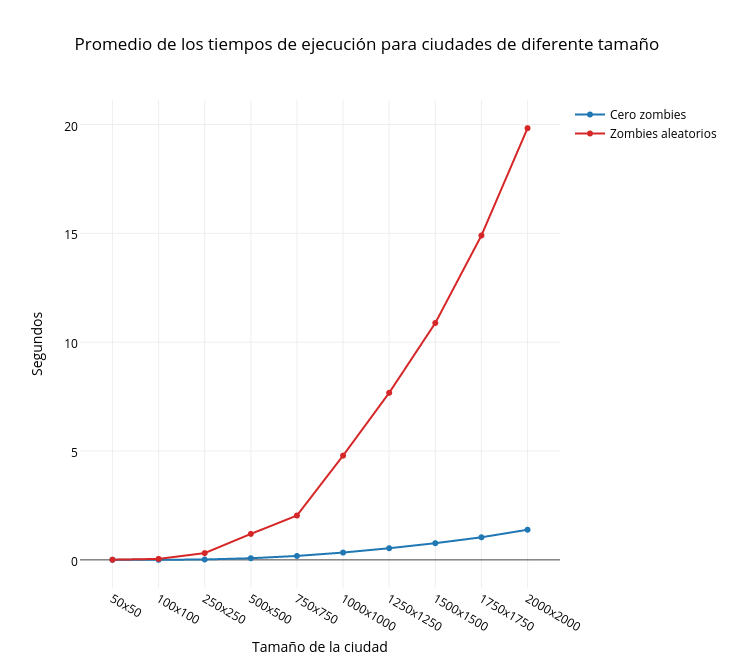
\includegraphics[width=15cm,keepaspectratio=yes]{imagenes/ej2/czyza.png}

Aquí se pueden apreciar las diferencias de tiempos. Ésta radica en el hecho de que \textbf{Zombies aleatorios} posee caminos en los cuales los soldados mueren. Por ello, el algoritmo deberá recorrer, en peor caso, $s$ veces la ciudad entera.\\

Se procedió, entonces, a dividir los resultados de \textbf{Zombies aleatorios} por la cantidad de soldados iniciales con los que se ejecutó el algoritmo a fin de que quede reflejado, que en ese caso, los tiempos serán muy similares a los de \textbf{Cero zombies}. Esto se debe a que ya no son los tiempos de recorrer $s$ veces la ciudad, sino de recorrerla una sola vez.
Sin embargo, es necesario aclarar que la similitud que se intenta mostrar, es aproximada, ya que no podemos asegurar que efectivamente, el algoritmo recorre $s$ veces la ciudad. Tal es el peor caso, y como hemos expuesto en un principio, no podemos asegurar que sea el que realmente ocurre.

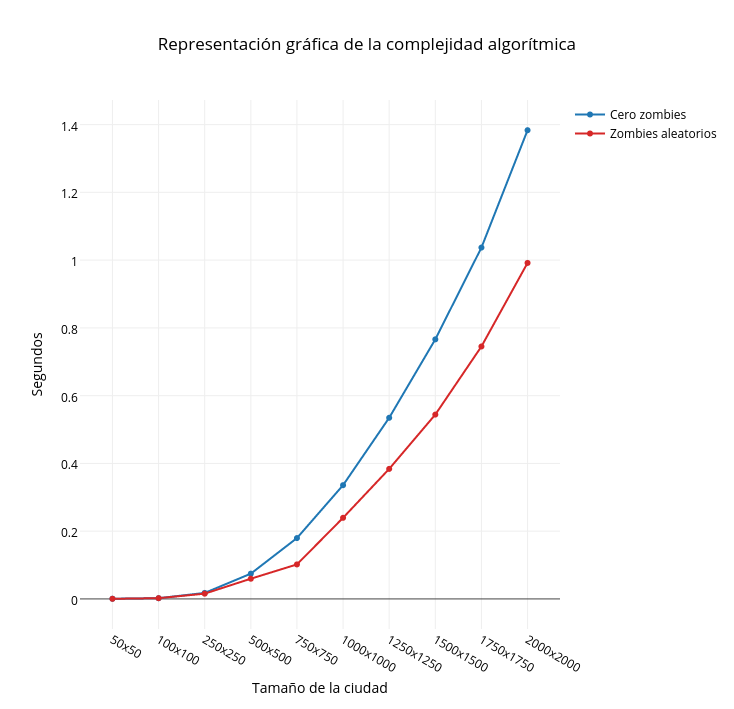
\includegraphics[width=15cm,keepaspectratio=yes]{imagenes/ej2/zaczados.png}

Manteniendo los resultados de \textbf{Zombies aleatorios} divididos por $s$, finalmente dividimos los resultados tanto de \textbf{Cero zombies} como de \textbf{Zombies aleatorios}, por $n$, y en una instancia aparte, por $n.m$.
De esta manera, dado que en ambos tienen $s$ igual a 1, solo queda ver que al dividir por $n$, los resultados se aproximan a una función lineal, y que al dividirlos por $n.m$, se aproximan a una constante.\\

Como solo nos interesa la relación, y no la función exacta ni la constante, multiplicamos los resultados de dichas divisiones por 100, para que los valores sean más claros y visibles.

\includegraphics[width=15cm,keepaspectratio=yes]{imagenes/ej2/linealizacion.png}

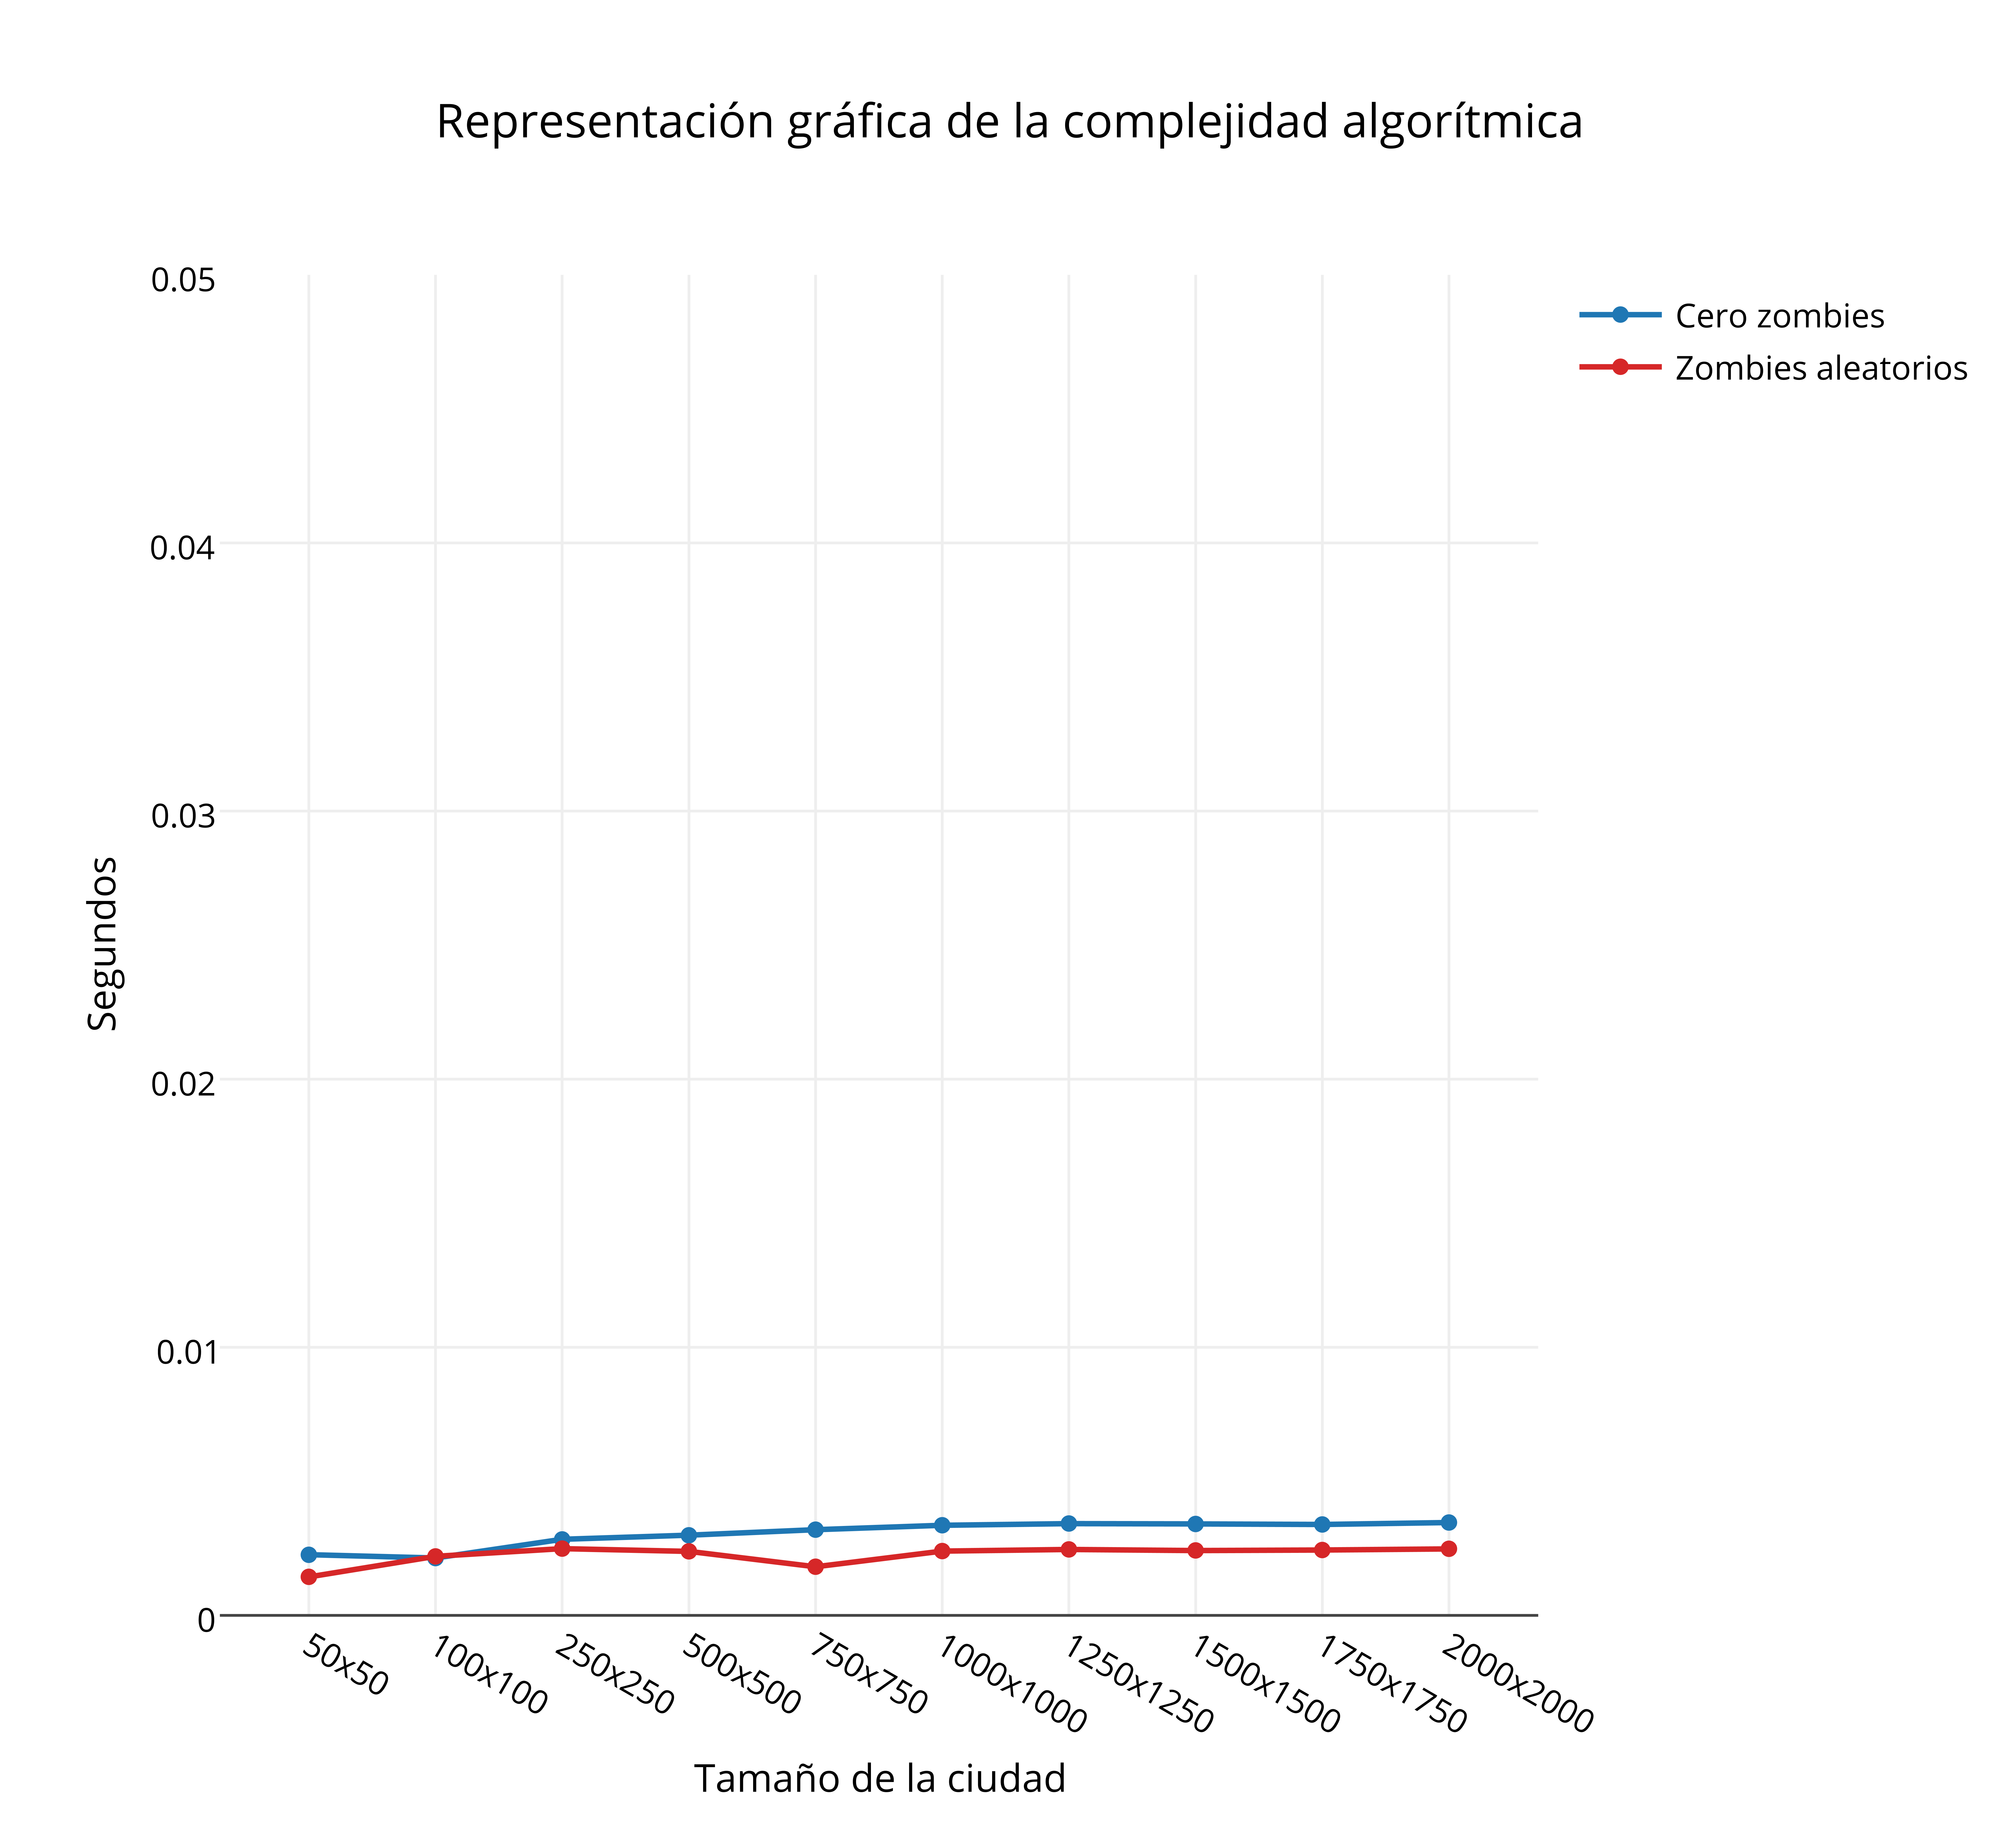
\includegraphics[width=15cm,keepaspectratio=yes]{imagenes/ej2/constantizacion.png}

Se puede ver que la experimentación se corresponde con la teoría, y que la complejidad, en peor caso, es $O(s.n.m)$.


\newpage
%\section{Heur\'istica Constructiva Golosa} \label{ej3}
\subsection{Explicaci\'on}
La heurística constructiva golosa busca, dado un grafo, determinar un conjunto independiente dominante mínimo. 

Para ello, el algoritmo ordena los nodos de acuerdo al grado de cada uno de ellos, de mayor a menor. Este orden se establece al comienzo de la ejecución y no se actualiza.\\

Luego, recorre dichos nodos, y por cada uno de ellos, lo agrega al conjunto solución, y va eliminando a sus vecinos, hasta que no quedan más nodos.\\

De esta manera, el algoritmo siempre obtiene un conjunto independiente (dado que por cada nodo que toma, elimina a sus vecinos) y dominante (dado que por cada nodo que toma, lo agrega al conjunto, y elimina a sus vecinos, es decir, que estos son adyacentes a un nodo del conjunto), pero no puede asegurar que siempre sea mínimo. Eso dependerá del grafo.\\

\textcolor{red}{Falta una explicacion mas detallada (un pseudocodigo, o algo), y aclarar que es goloso porque en cada paso elige la mejor opcion y nosostros definimos MEJOR como el mayor grado total}
%Explicar detalladamente el algoritmo implementado.

\newpage
\subsection{Complejidad Temporal}\label{compej3}
\textcolor{red}{Aca no me meto, todavia...}

En lo que respecta a la complejidad temporal, demostraremos a continuación que la misma es $O(n^{2})$ en la cantidad de nodos del grafo.\\

Recordemos que el algoritmo ordena los nodos de mayor grado a menor grado, luego toma el primero de dicha lista, lo agrega al conjunto solución, y lo elimina de la lista junto a sus adyacentes. Luego repite el proceso, tomando el siguiente nodo de la lista de nodos restantes.\\
Dicho esto, definiremos a $f(i,n): \mathbb{N} \rightarrow \mathbb{N}$ como:

$f(i,n)$ = Cantidad de operaciones en el peor caso, teniendo $n$ nodos totales y faltando eliminar $i$.\\
Es decir,\par
\begin{itemize}
	\item$f(0,n) = c$, dado que no falta eliminar ningun nodo, el algoritmo termina, con $c$ alguna cantidad constante de operaciones.\par
	\item $(\forall i \in {1...n-1}) f(i,n) = h*(i-1) + f(i-1,n) + c$, con $h$ la cantidad de vecinos del nodo que estoy viendo, $c$ alguna cantidad constante de operaciones, y $f(i-1,n)$ es el llamado recursivo.\\
\end{itemize}
Expliquemos que significa cada monomio:
\begin{itemize}
	\item $h*(i-1)$: En el peor de los casos, recorre por cada nodo de la lista de adyacencia del nodo tomado, a los demas nodos sin marcar (sin incluir el nodo tomado).
	\item $f(i-1,n)$: En el peor de los casos, no hay nodos de la lista de adyacencia, que no hayan sido eliminados aún.
	\item $c$: Alguna cantidad constante de operaciones.
\end{itemize}
Entonces, querremos demostrar que $(\forall i \in {1...n-1}) f(i,n) \leq k*i*n + c$ (con $k$ y $c$ alguna constante), pues al momento de ejecutar el algoritmo, se tienen $n$ nodos, y faltan eliminar $n$ nodos, siendo la complejidad del mismo, $O(f(n,n)) = O(n^{2})$; y dado que la cantidad de nodos por borrar no puede ser mayor que la cantidad total de nodos, es correcto pedir que $0 \leq i < n$.\\

\newpage
{\large\textbf{Teorema}}\\
Dado $f(i,n): \mathbb{N} \rightarrow \mathbb{N}$ definida como\\
$f(i,n)$ = Cantidad de operaciones  en el peor caso, teniendo $n$ nodos totales y faltando eliminar $i$.\\
$f(0,n) = c$\\
$f(i,n) = h*(i-1) + f(i-1,n) + c$\\
Luego, $(\forall i \in {1...n-1}) f(i,n) \leq k*i*n + c$.\\

{\large\textbf{Demostración}}\\
Sea $P(i) = f(i,n) \leq k*i*n + c$, demostraremos por inducción global, que $(\forall i \in {1...n-1}) P(i)$\\
Entonces,\\
\textbf{Casos base:}
\begin{itemize}
    \item[•] $f(0,n) = c$
    \item[•] $f(1,n) = h*(1-1) + c = c \leq k*1*n + c$\\
    Dado que tengo $n$ nodos, y solo falta eliminar uno. $k$ es alguna cantidad constante de operaciones para eliminar el nodo y finalizar el algoritmo.
\end{itemize}
\textbf{Paso inductivo:}\\

$\underbrace{P(1) \wedge P(2) \wedge ... \wedge P(m-1)}_{\text{Hipótesis inductiva}} \Rightarrow \underbrace{P(m)}_{\text{Tesis inductiva}}$\\

Es decir, que por hipótesis inductiva, podemos suponer que vale $f(r,n) \leq k*r*n + c$, con $r \leq m-1$, y queremos ver que $f(m,n) \leq k*m*n + c$.\\
Luego,
\begin{align*}
f(m,n) & = h*(m-1) + f(m-1,n) + c \\
 \stackrel{HI}{\Longrightarrow} f(m,n) & \leq h*(m-1) + n*(m-1) + c \\
 \intertext{Dado que la cantidad de vecinos adyacentes esta acotada por la cantidad de nodos totales, $0 \leq h < n$, luego}
 & \leq n*(m-1)+n*(m-1) + c\\
 & \leq n*m + n*m + c\\
 & = 2*n*m + c\\
 & \leq \underbrace{k*n*m + c}_{\text{Tesis inductiva}} \text{       En particular, con $k = 2$ en este caso}
\end{align*}
\hfill $\blacksquare$

Entonces, $f(i,n) \leq c*i*n + k$, para algún $c$ y $k$ constantes.
Dado que el algoritmo ejecuta, en peor caso, $f(n,n)$ operaciones, su complejidad esta acotada por $f(n,n)$, por lo tanto, tiene complejidad $O(n^{2})$.\\

También es adecuado decir, que el algoritmo tiene complejidad $\Omega(n*log(n))$, dado que debe ordenar los nodos de acuerdo al grado de cada uno, y cualquier algoritmo de ordenamiento basado en el árbol de decisiones no posee mejor complejidad que la mencionada.

%Calcular el orden de complejidad temporal de peor caso del algoritmo.
\subsection{Comparaci\'on de resultados con soluci\'on \'optima}
La heurística constructiva golosa fallará en encontrar la solución óptima para todos los casos.
Particularmente, existen grafos para los cuales la heurística fallará siempre.\\
Algunos de ellos son:
\textcolor{red}{Insertar nodo radial}

En este ejemplo, el greedy tomará como primer nodo, al nodo del centro, y eliminará a todos sus adyacentes. Luego, tomará todas las componentes conexas restantes.
El resultado final será una solución con $(m-2)*m$ versus $m$ de la solución óptima.

\textcolor{red}{Insertar mas ejemplos... Ayuda...}

%Describir instancias de CIDM para las cuales la heuristica no proporciona una solucion optima. Indicar que tan mala puede ser la solucion obtenida respecto de la solucion optima.
\subsection{Experimentaci\'on}
%Realizar una experimentacion que permita observar la performance del algoritmo en terminos de tiempo de ejecucion en funcion de los parametros de la entrada.
Para la experimentación, se realizaron experimentos sobre grafos generados de manera aleatoria, fijando nodos y variando ejes, y viceversa.

A continuación se adjuntan los gráficos con los resultados:

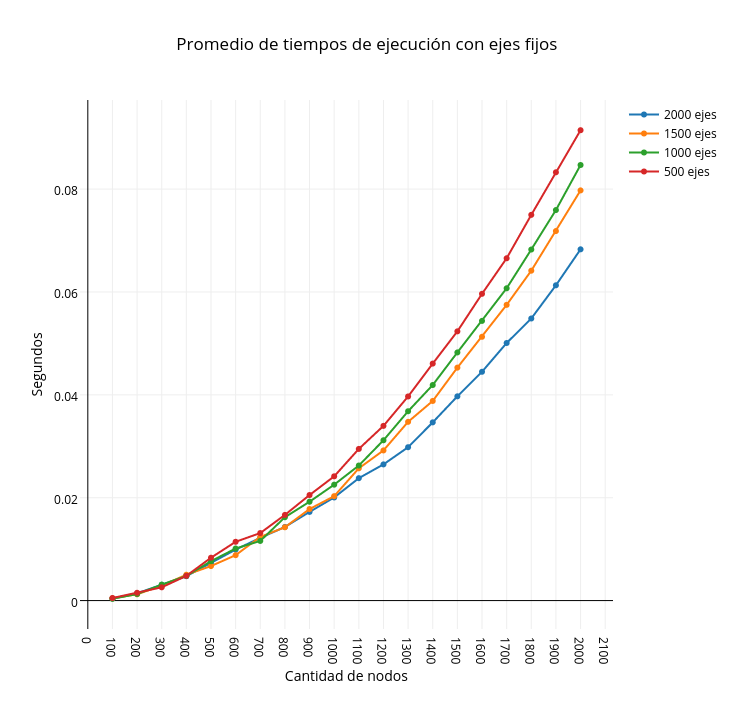
\includegraphics[width=15cm,keepaspectratio=yes]{imagenes/greedy/fixedge.png}

Como se puede observar, los tiempos aumentan a medida que disminuyen la cantidad de ejes. Esto se debe a que a menor cantidad de ejes, menor cantidad de nodos se eliminan de la lista de nodos que itera el algoritmo.

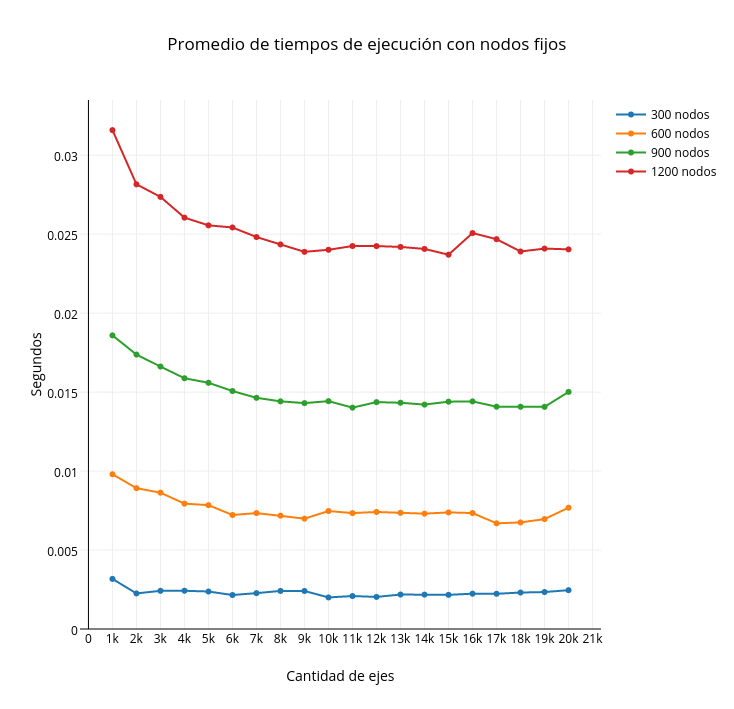
\includegraphics[width=15cm,keepaspectratio=yes]{imagenes/greedy/fixnode.png}

En este gráfico, se puede ver que si bien la cantidad de ejes (como fue mencionado en el gráfico anterior) afecta los tiempos, a mayor cantidad de ejes se puede observar que el verdadero limitante es la cantidad de nodos. Aquí se aprecia que la complejidad teórica se corresponde, en cuanto a que depende de la cantidad de nodos, y no de la cantidad de ejes.

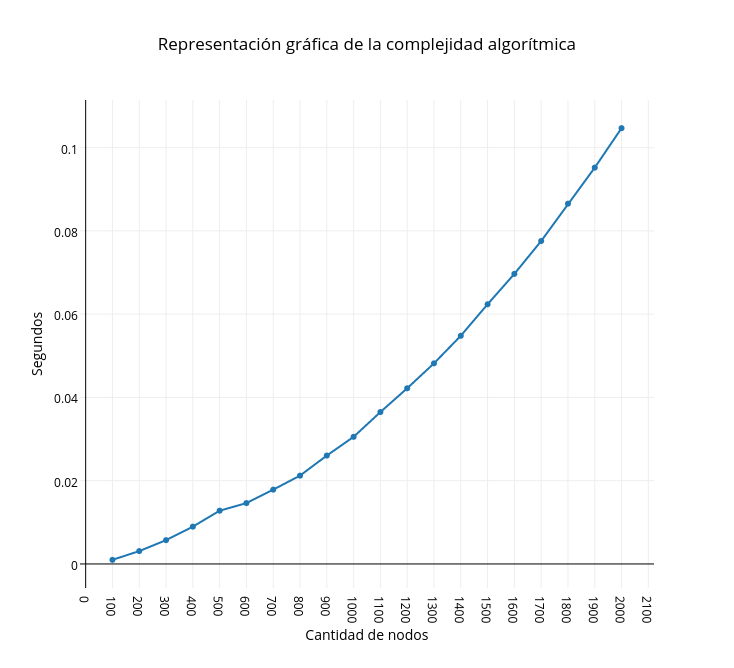
\includegraphics[width=15cm,keepaspectratio=yes]{imagenes/greedy/worst1.png}

Resultó interesante graficar, a su vez, algún caso en el que se refleje la complejidad algorítmica.
Para ello, se tomo el grafo sin ejes, es decir, todas componentes conexas, puesto que el algoritmo deberá recorrer, por cada nodo, el resto de todos los nodos preguntando si son vecinos.
Aquí se puede apreciar que efectivamente, los tiempos incrementan de manera cuadrática.

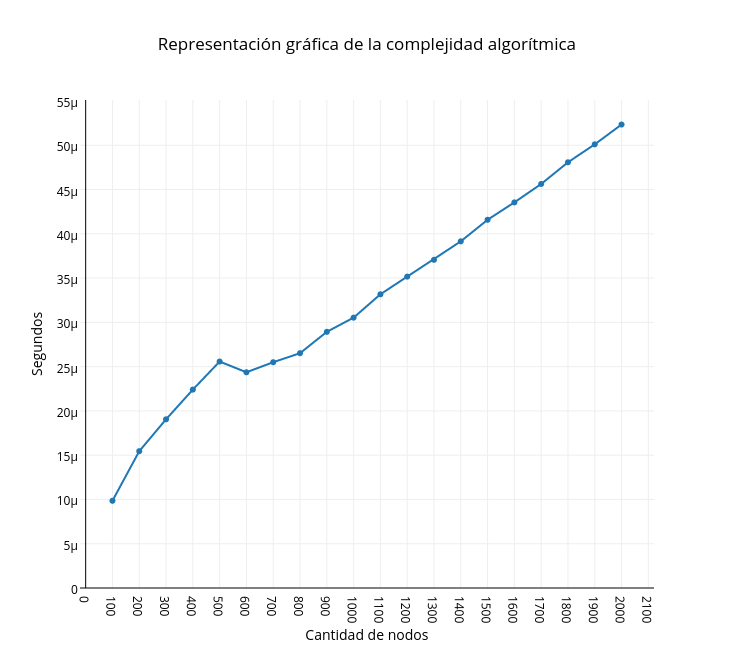
\includegraphics[width=15cm,keepaspectratio=yes]{imagenes/greedy/worst2.png}

Para asegurarnos de que efectivamente la función corresponde a la familia de funciones cuadráticas y no a otra, se procedió a dividir los resultados por el tamaño de la entrada.
Se puede apreciar que el gráfico se aproxima a una función lineal.

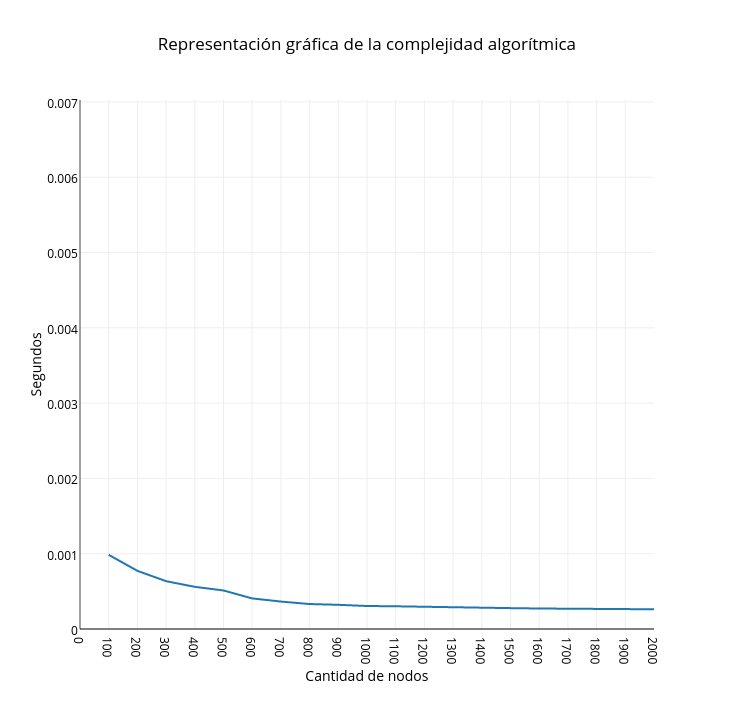
\includegraphics[width=15cm,keepaspectratio=yes]{imagenes/greedy/worst3.png}

Finalmente, se procedió a dividir los resultados (ya divididos) por el tamaño de la entrada nuevamente.
Efectivamente, el resultado tiende a una constante, lo que termina demostrando de manera empírica, la complejidad teórica explicada.
\newpage
\section{Heur\'istica de B\'usqueda Local} \label{ej4}

Un algoritmo de Búsqueda Local consiste en dos simples pasos: elegir una solución inicial y luego, \textcolor{red}{Aca explicarlo bien, esta horrible} iterar


modificarla (``mejorandola''), reemplazándola paso a paso con distintas soluciones que pertenezcan a la vecindad de la misma.


Para cada solución factible s $\epsilon$ S se define N(s) como el conjunto de
``soluciones vecinas'' de s. Un procedimiento de busqueda local toma una solución inicial s e iterativamente la mejora reemplazándola por otra solución mejor del conjunto N(s), hasta llegar a un óptimo local.

 Sea s $\epsilon$ S una solución inicial
 
 Mientras exista s $\epsilon$ N(s) con f (s) $>$ f (s)
 
 s $\leftarrow$ s


\subsection{Explicaci\'on}
%Explicar detalladamente el algoritmo implementado. Plantear al menos dos vecindades distintas para la busqueda y al menos dos soluciones iniciales.

Considerando el problema a tratar, establecimos nuestros criterios para encontrar las soluciones iniciales y las vecindades.\\


\subsubsection{Elección de Solución Inicial}

Al momento de seleccionar la solución Inicial, determinamos dos criterios.

\subsubsection*{Criterio I Solución Inicial: Golosa}

Se realiza una ejecución del algoritmo Goloso de la Sección \ref{ej3}.\\

Esto quiere decir, se ordenan los nodos por grado de manera decreciente. Se eligen los nodos de a uno (de mayor a menor), de modo que al elegir un nodo se descartan sus vecinos para sus futuras elecciones.

\subsubsection*{Criterio II Solución Inicial: Secuencial}

Los nodos al ser ingresados como parámetro del algoritmo tienen como identificador un número entre $0$ y $n-1$. El orden que vamos a utilizar para recorrerlos es el que haya sido dado cuando fueron ingresados como parámetro.\\

Lo primero que realizamos es tomar al nodo $0$ y considerarlo parte de la solución. Se descartan todos los nodos vecinos a él y se continúa el proceso con el nodo que tenga menor número de \textit{id}.

De este modo se forma un conjunto solución tal que en cada paso añade al nodo disponible que tenga su identificador número menor.

\subsubsection{Elección de Vecindad}

Dada una soluci\'on al problema, se establece un conjunto de soluciones ``similares'' denominadas \emph{vecinas}. Los criterios para elegir esta vecindad pueden variar.

\subsubsection*{Criterio I Vecindad}

El primer criterio elegido es, a partir de una soluci\'on, quitarle dos nodos y agregarle uno que no haya sido contenido.\\

Para ello, se prueban todas las combinaciones de pares de nodos dentro del conjunto posibles y se considera a los nodos que tienen ambas como vecinos. Si al sacar este par y agregar el nuevo nodo, se obtiene un conjunto Independiente Dominante M\'inimo, se actualiza el conjunto soluci\'on. 

\subsubsection*{Criterio II Vecindad}

El segundo criterio es similar al anterior, s\'olo que ahora consideramos quitar tres nodos y agregar uno.\\

Se consideran todas las combinaciones posibles de grupos de tres nodos dentro del conjunto soluci\'on inicial y se prueba con los nodos que sean vecinos de todos ellos si forman un conjunto soluci\'on.\\

\textcolor{red}{Las opciones que elegimos son: 2, 3, 4 y 5 y son BLABALLABLA}

\newpage
\subsection{Complejidad Temporal}
%Calcular el orden de complejidad temporal de peor caso de una iteracion del algoritmo de busqueda local (para las vecindades planteadas). Si es posible, dar una cota superior para la cantidad de iteraciones de la heurıstica.
Este algoritmo llama, seg\'un la vecindad a ejecutar, a una de las siguiente dos funciones, que dominan la complejidad del ciclo.

\subsubsection{dameParesVecinosComun}\label{vec1}

Funciones usadas:\\
listaAd::dameVecinos\\
push_back\\
size\\

Dado un conjunto de nodos, se buscan todas las combinaciones de pares de nodos posibles. 
Luego, para cada par de nodos (i,j) se recorren: la lista de adyacencia de i y la de j. 
Por cada elemento que pertenezca a las dos listas, se a\~nade al vector \texttt{vecinosEnComun} dentro de la estructura pares.

\begin{algorithm}[h!]
struct vecinosEnComun\{\\
	unsigned int nodoA;\\	
	unsigned int nodoB;\\
	vector<unsigned int> vecinosComun;\\
\};
\end{algorithm}

\begin{algorithm}[h!]
	\For{int i = 0; i $<$ optimo.size(); ++i}{
		\For{int j = i+1; j $<$ optimo.size(); ++j}{
			list$<$unsigned int$>$* vecinosA = adyacencia.dameVecinos(optimo[i]);\\
			list$<$unsigned int$>$* vecinosB = adyacencia.dameVecinos(optimo[j]);\\
			vecinosEnComun par;\\
			par.nodoA = optimo[i];\\
			par.nodoB = optimo[j];\\
			list$<$unsigned int$>$::iterator itVecinosA = vecinosA-$>$begin(), itVecinosB = vecinosB-$>$begin();\\
			\While{itVecinosA != vecinosA-$>$end() and itVecinosB != vecinosB-$>$end()}{
				\eIf{*itVecinosA == *itVecinosB}{
					par.vecinosComun.push_back(*itVecinosA);\\
					itVecinosA++;\\
					itVecinosB++;\\
				}{
					\eIf{*itVecinosA $>$ *itVecinosB}{
						itVecinosB++;
					}{
						itVecinosA++;
					}
				}
			}
			\If{par.vecinosComun.size() $>$ 0}{
				pares.push_back(par);
			}
		}
	}
\end{algorithm}

Para elegir todos los pares posibles de nodos en el conjunto \texttt{\'optimo}, se recorre mediante dos \emph{for}s.\\
El primero itera i desde 0 hasta el \'ultimo elemento y el segundo desde i hasta el \'ultimo elemento.\\
De este modo, cada par de nodos se recorre una \'unica vez. Ya que es lo mismo el par (i,j) que (j,i).\\

Dentro de los \emph{for}s anidados, se crea una estructura \texttt{vecinosEnComun} \textbf{par} donde el nodoA es i y el nodoB es j.\\

Para poder armar la lista vecinosComun (miembro de la estructura vecinosEnComun), se iteran las listas de adyacencia con itVecinosA (i) e itVecinosB (j).\\

Como ambas listas fueron ordenadas antes de invocar a la funci\'on dameParesVecinosComun, es posible encontrar elementos en com\'un recorriendolas secuencialmente de manera simult\'anea.\\

Se procede de manera simple, si nodo(itVecinosA) es igual a nodo(itVecinosB) entonces se a\~nade el nodo actual a la lista vecinosComun.\\

En caso contrario, se avanza el iterador que sea menor.\\

Si conclu\'ida la iteraci\'on de las dos listas de adyacencia, la lista vecinosEnComun posee al menos un elemento; entonces se agrega \textbf{par} a la soluci\'on.

Dado un par (i,j), la complejidad de recorrer ambas listas de adyacencia es de: $O(grado(i)+grado(j))$.
Cada par se recorre una \'unica vez. Por lo tanto, los dos \emph{for}s anidados van a iterar (considerando a (n-1) como el \'ultimo nodo'):\\

Cuando sea el par de nodos (0,1) : grado(0)+grado(1) \\

Cuando sea el par de nodos (0,2) : grado(0)+grado(2) \\

...\\

Cuando sea el par de nodos (0,n-1) : grado(0)+grado(n-1)\\

Cuando sea el par de nodos (1,2) : grado(1)+grado(2)\\

Cuando sea el par de nodos (1,3) : grado(1)+grado(3)\\

...\\

Cuando sea el par de nodos (1,n-1) : grado(1)+grado(n-1)\\

...\\

Cuando sea el par de nodos (n-2,n-1) : grado(n-2)+grado(n-1)\\


Se puede apreciar que el grado de cada nodo se suma (n-1) veces. Por lo tanto, al sumar las complejidades da un total de:\\

grado(0)*(n-1) + grado(1)*(n-1) + ... + grado(n-1)*(n-1)\\

lo que es equivalente a:\\

[grado(0)+grado(1)+ ... + grado(n-1)]*(n-1)\\

La complejidad en peor caso se obtiene cuando los grados de todos los nodos son maximos, por lo tanto se trata de un grafo completo.
Donde vale que 2*\#ejes = grado(0)+grado(1)+ ... grado(n-1).\\

Por consecuencia, la complejidad de esta funci\'on es de:\\

O(2*\#ejes*(n-1)) lo que equivale a O(\#ejes*n) que pertenece a O($n^3$) ya que la mayor cantidad de ejes que puede tener un grafo es ((n-1)n)/2


\subsubsection{dameTernasVecinasComun}\label{vec2}

La funci\'on dameTernasVecinasComun funciona de manera an\'aloga a la descripta en el inciso \ref{vec1}.\\

Se va a encargar de armar tomar de todas las maneras posibles tres nodos del conjunto pasado por par\'ametro.\\

Luego, obtener los nodos (si existe) que sean vecinos de los tres.\\

De esta manera, recorre el conjunto con tres \emph{for}s tal que cada tupla la recorre una sola vez.\\

En este caso el c\'alculo de cada iteraci\'on, dada la tupla (i,j,k), ser\'a de grado(i)+grado(j)+grado(k).\\

Dada la tupla (0,1,2) el costo ser\'a: grado(0)+grado(1)+grado(2)\\

Dada la tupla (0,1,3) el costo ser\'a: grado(0)+grado(1)+grado(3)\\

...\\

Dada la tupla (0,1,n-1) el costo ser\'a: grado(0)+grado(1)+grado(n-1)\\

Dada la tupla (0,2,3) el costo ser\'a: grado(0)+grado(2)+grado(3)\\

...\\

Dada la tupla (0,n-2,n-1) el costo ser\'a: grado(0)+grado(n-1)+grado(n-2)\\

Dada la tupla (1,2,3) el costo ser\'a: grado(1)+grado(2)+grado(3)\\

...\\

Dada la tupla (n-3,n-2,n-1) el costo ser\'a: grado(n-3)+grado(n-2)+grado(n-1)\\

En el peor caso, el grado de todos los nodos es de n (grafo completo). Por lo tanto, el costo de cada iteraci\'on es de O(3n).\\

La cantidad de ternas que se pueden formar es de $(n(n-1)(n-2))/6$, equivale a decir que va a iterar $O(n^3)$ veces con costo $O(3n)$ cada vez.\\

Dando una complejidad de $O(n^4)$.

\newpage
\subsubsection{localCIDM}
Como primera medida, ordena todas las listas de adyacencia: listaAd::ordenar, esto toma $O(n^2.log(n))$, para cada nodo ($n$) ordenar su lista de adyacencia (en el caso del grafo completo, tendr\'an ($n-1$) vecinos, y ordenarlos toma $O(n.log(n))$)\\

Para las \textbf{ejecuciones 3 y 5}, el parametro greedy esta en true, por lo tanto comienza con una solucion inicial golosa. Por lo tanto invoca a la funcion greedyCIDM() la cual tiene complejidad $O(n^2)$ explicada en el inciso \ref{ej3}.\\

\bigskip

Para las \textbf{ejecuciones 2 y 4}, la solucion inicial es secuencial. Esto quiere decir que para obtener una primera soluci\'on al problema se arma un vector \texttt{nodos} con la cantidad de nodos, donde en la posici\'on i se encuentra el nodo i.\\

Se recorre secuencialmente este arreglo (desde la posici\'on cero) de modo que se a\~nade el nodo actual a la soluci\'on y se elimina del vector \texttt{nodos}.\\

Luego, se borran tambi\'en del vector a los vecinos del nodo actual.\\

En la siguiente iteraci\'on se tienen $n-1-(grado(0))$ elementos en el vector \texttt{nodos}.\\

Lo cual, en el peor caso, ser\'ia n-1 donde grado(0)=0.\\

Considero la notaci\'on vecinos(i) como la cantidad de nodos pertenecientes al vector \texttt{nodos} durante la iteraci\'on i que sean adyacentes al nodo i.\\

En la iteraci\'on i, el vector va a contener $n-1-grado(0)- ... -1-vecinos(i)$\\

Donde en el peor caso, tambi\'en, deber\'a ser vecinos(i) con valor m\'inimo. Por consecuente, el peor caso es un grafo donde cada nodo es una componente conexa trivial, es decir que no existen ejes.\\
	
En el peor caso, itera n veces ya que el tama\~no del vector disminuye s\'olo en una unidad por iteraci\'on.\\

El costo de las operaciones por iteraci\'on es $O(n)$.\\

Las funciones usadas son:\\

push_back (costo $O(n)$ amortizado)\\

listaAdy::sonVecinos (costo $O(min(grado(nodoA), grado(nodoB)))$)\\

Por lo tanto esta seccion es del orden de O($n^2$)

\bigskip

A continuaci\'on, se introducen optimizaciones del algoritmo.

\begin{itemize}
\item En primer lugar, si la soluci\'on \'optima actual posee tama\~no 1 no va a encontrarse una soluci\'on mejor, por consiguiente se devuelve. (Costo $O(1)$)
\item En segundo lugar, si la soluci\'on \'optima actual posee tama\~no 2 la \'unica soluci\'on que puede ser mejor es la que posee un s\'olo nodo. Se chequea si existe una soluci\'on con un s\'olo nodo (costo $O(n)$). Si existe, la soluci\'on \'optima es la de un s\'olo nodo y se devuelve sino era la soluci\'on con dos nodos. Funciones usadas: assign, listaAdy::gradoDeNodo y listaAdy::cantNodos (todas con costo $O(1)$)
\item En tercer lugar, si la soluci\'on \'optima actual posee tama\~no n debe ser la soluci\'on que se retorne. Ya que la \'unica manera de que todos los nodos sean parte del conjunto soluci\'on al problema es que cada uno sea una componente conexa, es decir no existan ejes. A continuaci\'on, debe ser la soluci\'on devuelta. (Costo $O(1)$)
\end{itemize}

Si la ejecuci\'on del algoritmo no entr\'o en ninguno de los casos citados, se prosigue ordenando al vector de soluci\'on \'optima. (Costo $O(n.log(n))$, en el peor caso tiene $n-1$ elementos)\\

Ahora se prosigue con las iteraciones por vecindades.\\

En los casos de \textbf{ejecuci\'on 2 y 3}, se pasa por par\'ametro el valor de vecindad==true. Se ejecuta la funci\'on dameParesVecinosComun (vista en \ref{vec1}), es decir por cada iteraci\'on se querr\'a tomar un par de nodos tal que sea posible quitarlos y agregar un vecino de ambos al conjunto soluci\'on y se obtenga una soluci\'on con un nodo menos.\\

Se iterar\'a en un while hasta que la variable hayCambiosHechas sea false (complejidad $O(n)$ explicada m\'as adelante).\\

Lo primero que se hace es ejecutar \texttt{dameParesVecinosComun()} (complejidad $O(n^3)$).\\

Si esta funci\'on no devolvi\'o ning\'un par, se debe salir del ciclo.\\

Se ejecuta otro while, mientras haya pares sin ser visitados (de los obtenidos) (complejidad $O(n.(n-1)/2) = O(n^2)$).\\

Como lo que se quiere hacer es borrar nodos del conjunto soluci\'on, se hace en una copia porque a priori no se sabe si conducir\'a a un conjunto que sea soluci\'on.\\

Se borra del conjunto soluci\'on al par actual (i,j) que por el modo en que armamos los pares siempre se cumple que $i<j$. Esto tiene un costo de O(n) ya que itera la soluci\'on hasta que encuentre j y en el medio elimina i. Se borra con el operador \texttt{erase} de iterador (complejidad $O(3n) en el peor caso$).\\

Ahora resta ver si al agregar alg\'un nodo en com\'un se forma un conjunto soluci\'on que sea Independiente Maximal. Recorreremos la lista de nodos que tienen en com\'un i y j para ver si al agregar alguno de ellos al conjunto soluci\'on, el conjunto obtenido cumple ser Independiente Dominante M\'inimo. Es decir, se itera la lista de vecinos hasta encontrar un nodo que al insertarlo cumpla ser un conjunto soluci\'on v\'alido o hasta que termine sin haber podido formar un CIDM.\\

Lo que tendr\'a un costo de $O(n^2)$.\\

Primero se fija que esta combinaci\'on de quitar los nodos (i,j) y agregar el nodo actual no se haya probado todav\'ia, si es as\'i se agrega el nodo actual de la lista al conjunto soluci\'on de manera ordenada. Se itera el vector hasta la posici\'on donde se debe insertar lo que tiene costo de O(n) ya que en peor caso en la soluci\'on original hab\'ia n-1, se sacaron i y j por lo que el vector qued\'o de un tama\~	no n-2. Si el nodo a insertar debe hacerse al final, recorre todos.\\

iterator::insert tiene complejidad $O(n)$\\

Ahora con el conjunto formado se invoca a la funci\'on lisAdy::esIndependienteMaximal que tiene una complejidad de $O(n^2)$\\

Si el conjunto armado hasta el momento no es Independiente Maximal, vamos a querer borrar el nodo a\~nadido \'ultimo por lo que se itera de nuevo el vector hasta encontrarlo y borrarlo con iterator::erase con un costo total de O(n).\\

Este c\'odigo si al momento de quitar dos nodos (i,j) puede a\~nadir diversos nodos y con cualquiera resulta un conjunto Independiente Maximal, s\'olo considera al primero que logre cumplir ser un conjunto Independiente Maximal.\\

Si al quitar dos nodos y agregar uno se logr\'o un conjunto soluci\'on v\'alido se actualiza el vecotr soluci\'on \texttt{optimo}.\\

El ciclo mayor iterar\'a hasta que no se hagan m\'as cambios. Esto va a pasar cuando haya probado todos los pares de nodos posibles y por cada uno probado a\~nadir otro.\\

Es decir, en el peor caso se comenz\'o con una soluci\'on inicial de n-1 nodos y, se quitaron dos y a\~nadi\'o uno hasta que la soluci\'on final quede de tama\~no 1. Es decir, el while m\'as grande iterar\'a en peor caso n veces.\\

Por cada par de nodos iterar\'a $n^2$ veces y la cantidad de pares posibles en peor caso ser\'a de $O(n^2)$.\\

Por lo tanto el costo de cada iteraci\'on del ciclo mayor ser\'a de $O(n^4)$, iter\'andola n veces dar\'a un costo total del algoritmo de $O(n^5)$.\\

\bigskip	

En los casos de \textbf{ejecuci\'on 4 y 5}, el procedimiento ser\'a similar.\\

Primero buscar\'a ternas con vecinos en com\'un (\texttt{dameTernasVecinasComun}) con un costo de $O(n^4)$.\\

Pero el costo de cada iteraci\'on del ciclo mayor ser\'a de $O(n^4)$, por lo explicado anteriormente, con lo cual el costo total del algortimo es $O(n^5)$ tambi\'en para esta vecindad. 


\newpage
\subsection{Experimentaci\'on}
%Realizar una experimentacion que permita observar la performance del algoritmo comparando los tiempos de ejecucion y la calidad de las soluciones obtenidas, en funcion de las vecindades y las soluciones iniciales utilizadas y elegir, si es posible, la configuracion que mejores resultados provea para el grupo de instancias utilizado.

El objetivo de esta secci\'on es comparar los cuatro m\'etodos implementados bajo el paradigma de \emph{B\'usqueda Local} entre s\'i, respecto de su tiempo de ejecuci\'on y del conjunto soluci\'on resultante.

Adem\'as, las soluciones obtenidas por los cuatro m\'etodos se constrastan con la soluci\'on \'optima resultante de ejecutar el algoritmo exacto para las mismas instancias.\\

Todas las instancias utilizadas fueron generadas con el generador de instancias detallado en la Secci\'on \ref{instacegen}.

\subsubsection{An\'alisis de tiempos de ejecuci\'on}\label{tiempos}

En primera instancia, contrastamos tiempos de ejecuci\'on entre los cuatro m\'etodos. Como as\'i tambi\'en el crecimiento de la curva de tiempos de ejecuci\'on acorde var\'ian los ejes y los nodos dejando fijo nodos y ejes respectivamente.

\subsubsection*{Ejes Fijos}

Con el generador de instancias se armaron grupos de grafos con 100, 500, 2000 y 4000 ejes variando la cantidad de nodos. Se ejecutaron los cuatro m\'etodos para todos los casos generados.\\

Se midieron los tiempos de ejecuci\'on y se exponen a continuaci\'on:

  \begin{figure}[h!]
   \begin{center}
 	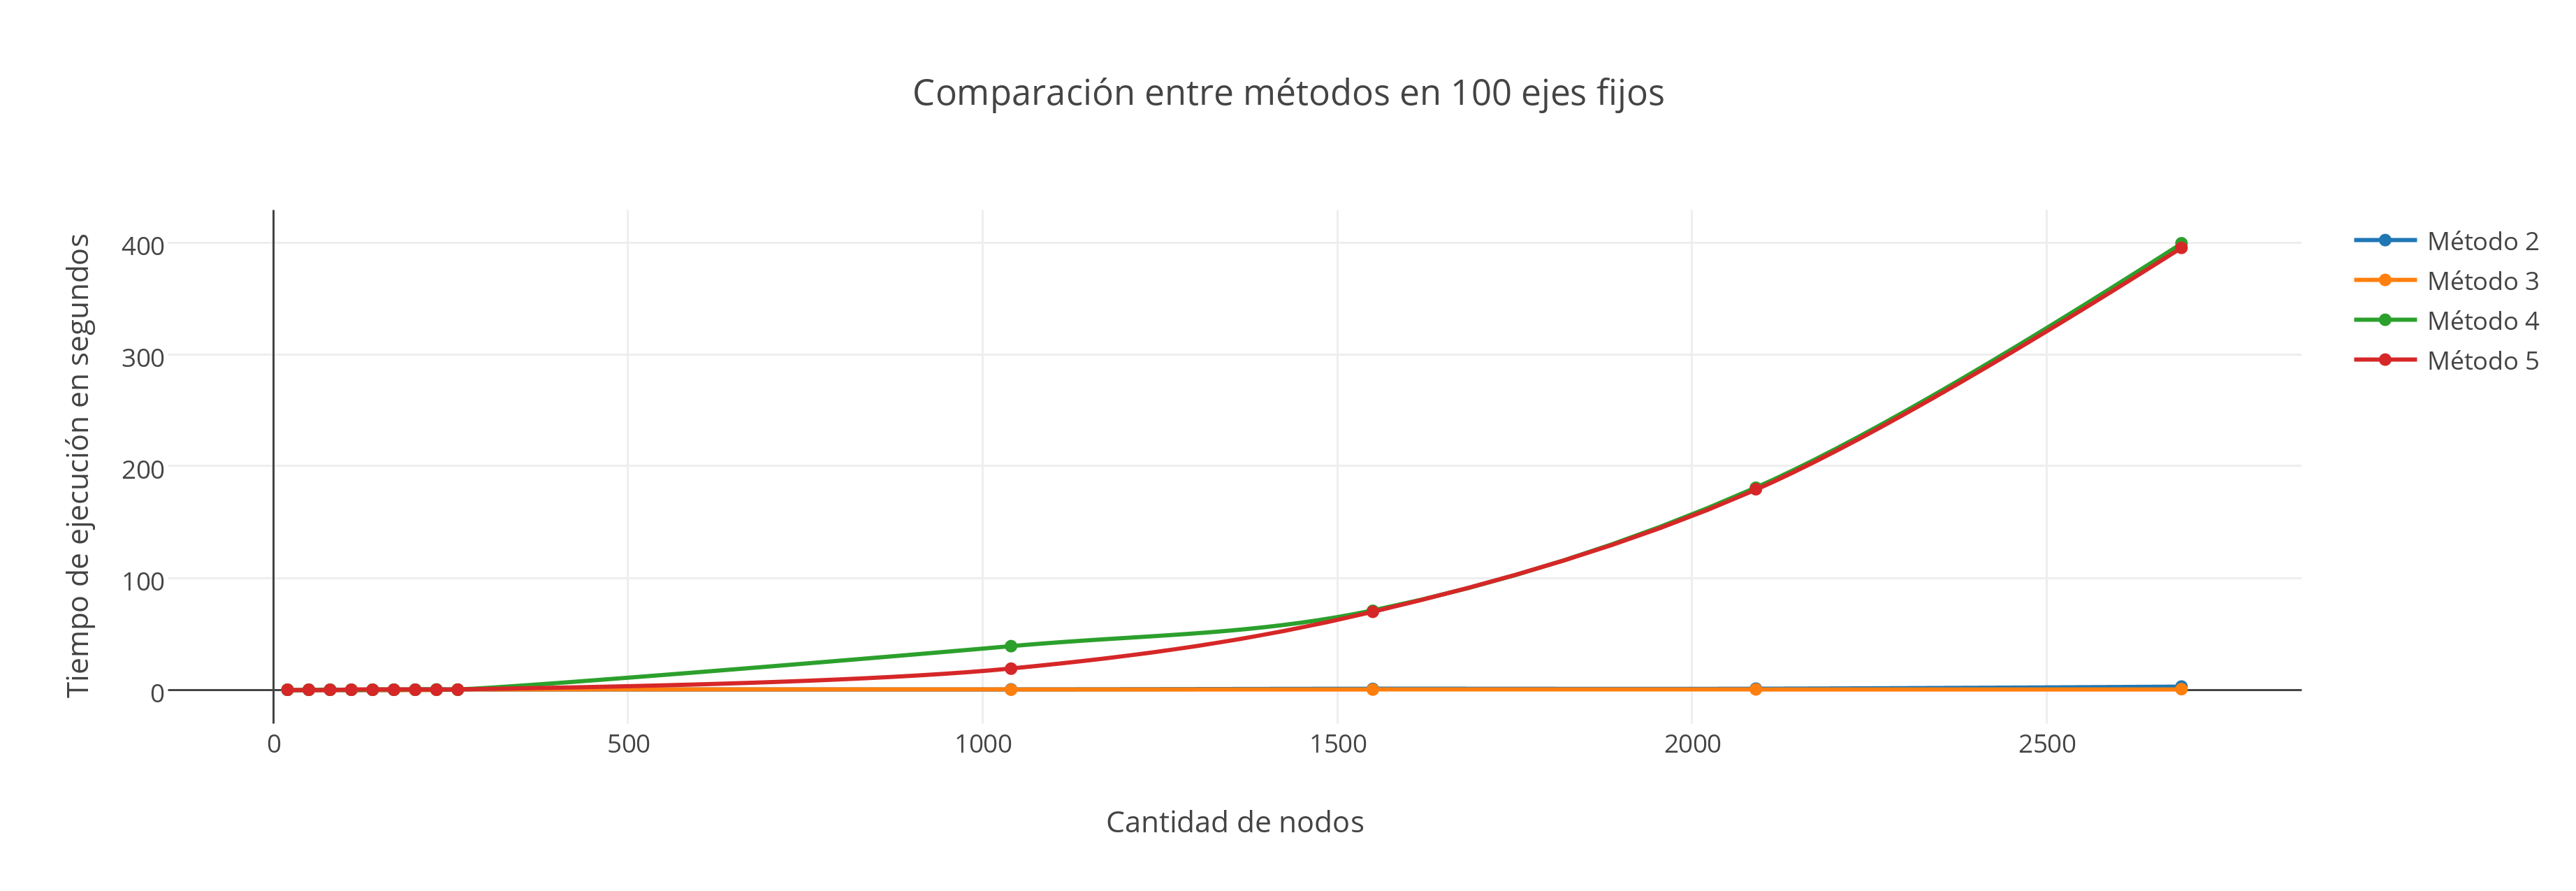
\includegraphics[scale=0.55]{imagenes/local/tiempos/100ejes.png}
% 	\caption{}
%	\label{10Nodos}
   \end{center}
 \end{figure}
 
  \begin{figure}[h!]
   \begin{center}
 	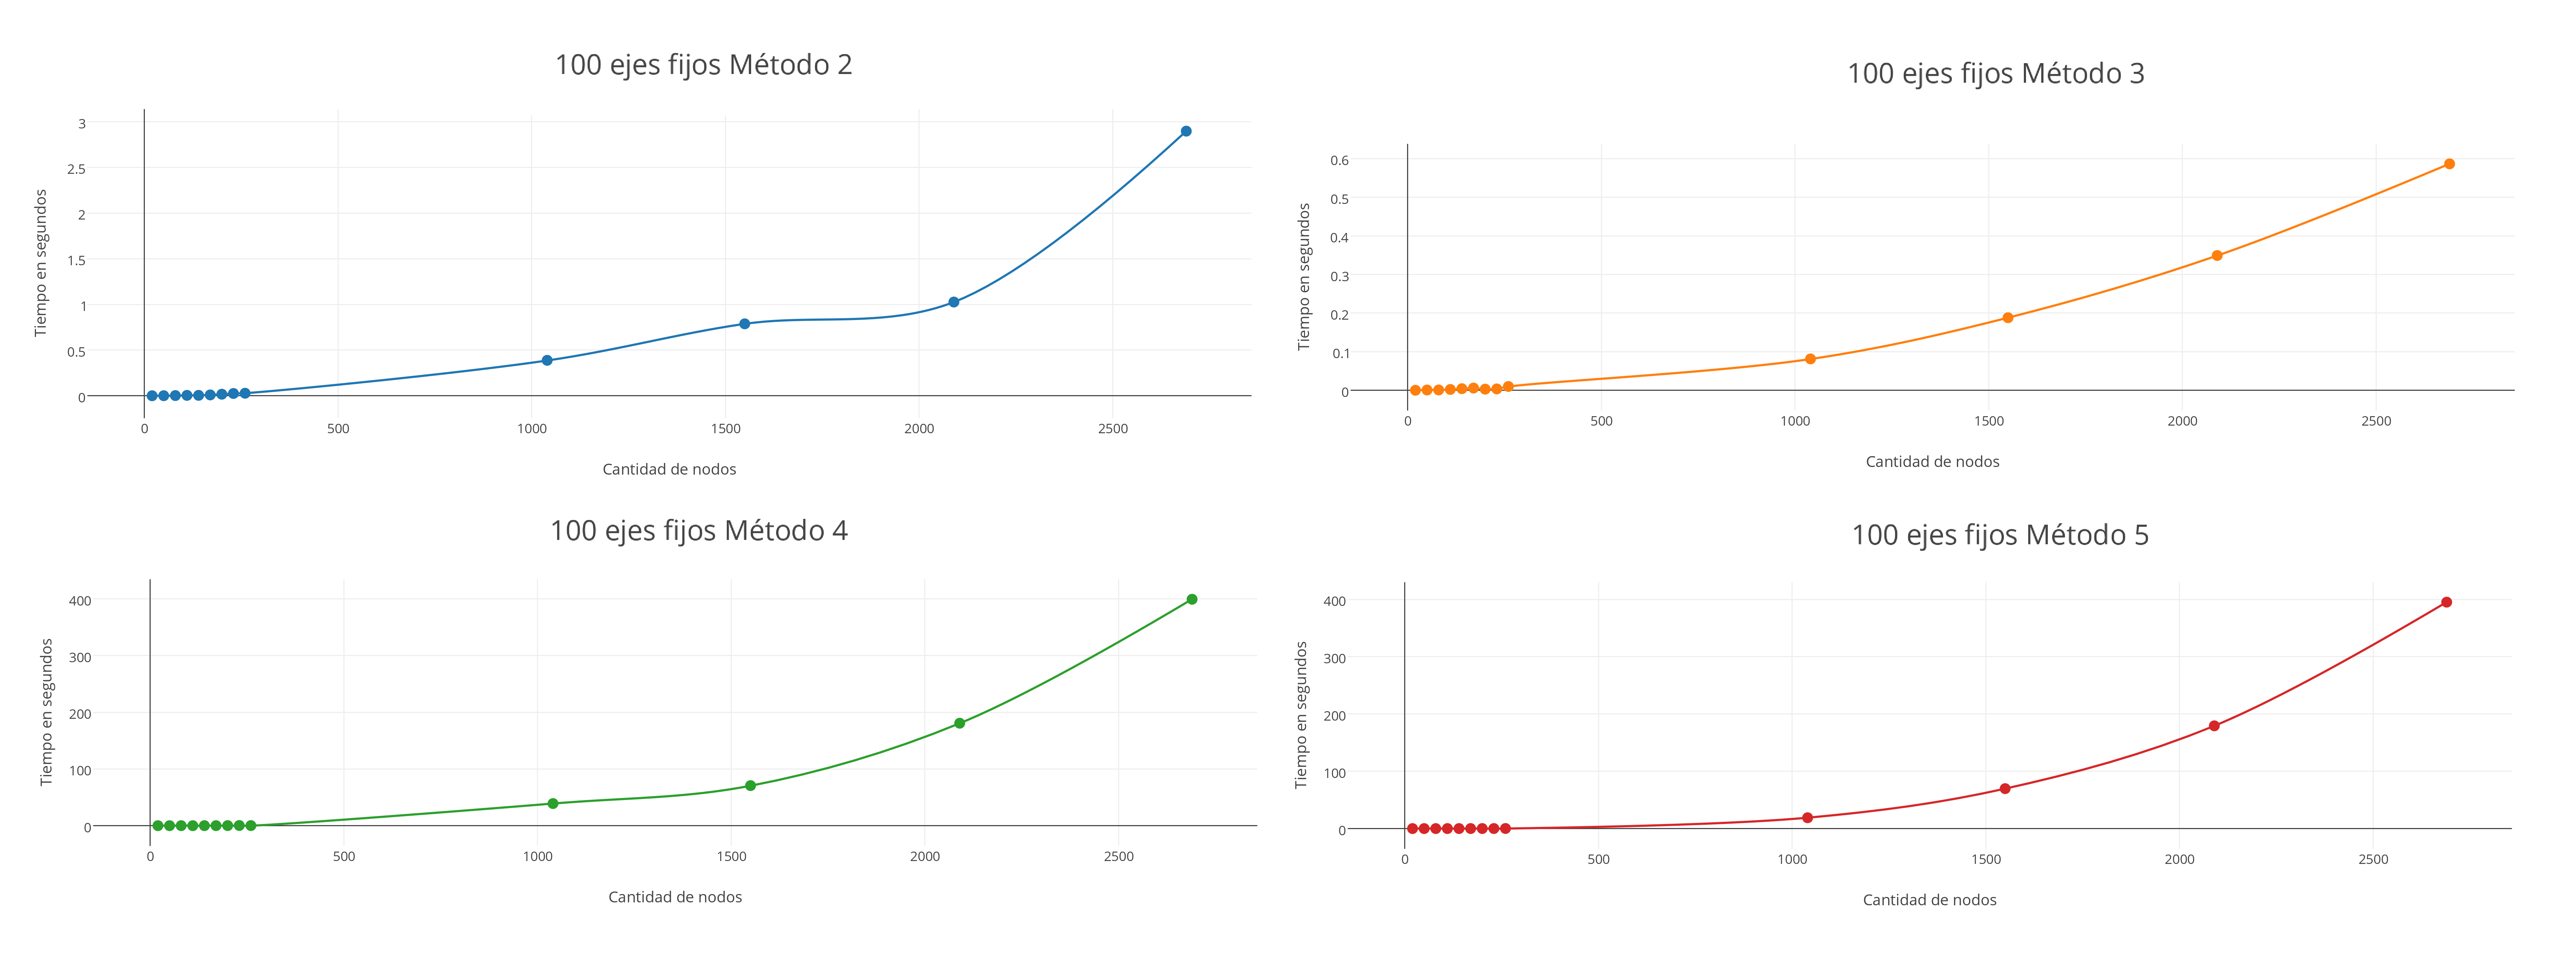
\includegraphics[scale=0.08]{imagenes/local/tiempos/100ejes2.png}
% 	\caption{}
%	\label{10Nodos}
   \end{center}
 \end{figure}

  \newpage  
 
En el primer gr\'afico se puede apreciar que cuando la cantidad de nodos comienza a ser mayor, los m\'etodos con la segunda vecindad (\textbf{4} y \textbf{5}) presentan una curva que posee un crecimiento mayor que las otras dos. Este comportamiento se condice con la complejidad te\'orica calculada ya que los m\'etodos 3 y 4 tienen una complejidad de \textcolor{red}{$O(n^6)$ (?} mientras que los primeros dos tienen \textcolor{red}{$O(n^5)$ (?}.\\

En el segundo gr\'afico lo que se quiso hacer es mostrar con detalle cada m\'etodo ya que en el primero, al tener cantidades de tiempo variadas, no se puede apreciar con detalle el comportamiento de todas las curvas por s\'i solas.

De este modo, se puede apreciar que los cuatro m\'etodos tienen un comportamiento que asemeja a una funci\'on \textcolor{red}{polinomial (? es asi?? nunca me acuerdo eso!)} aunque a simple vista no se podr\'ia acertar que sean las mismas funciones nombradas como complejidad.

\bigskip  
  
  \begin{figure}[h!]
   \begin{center}
 	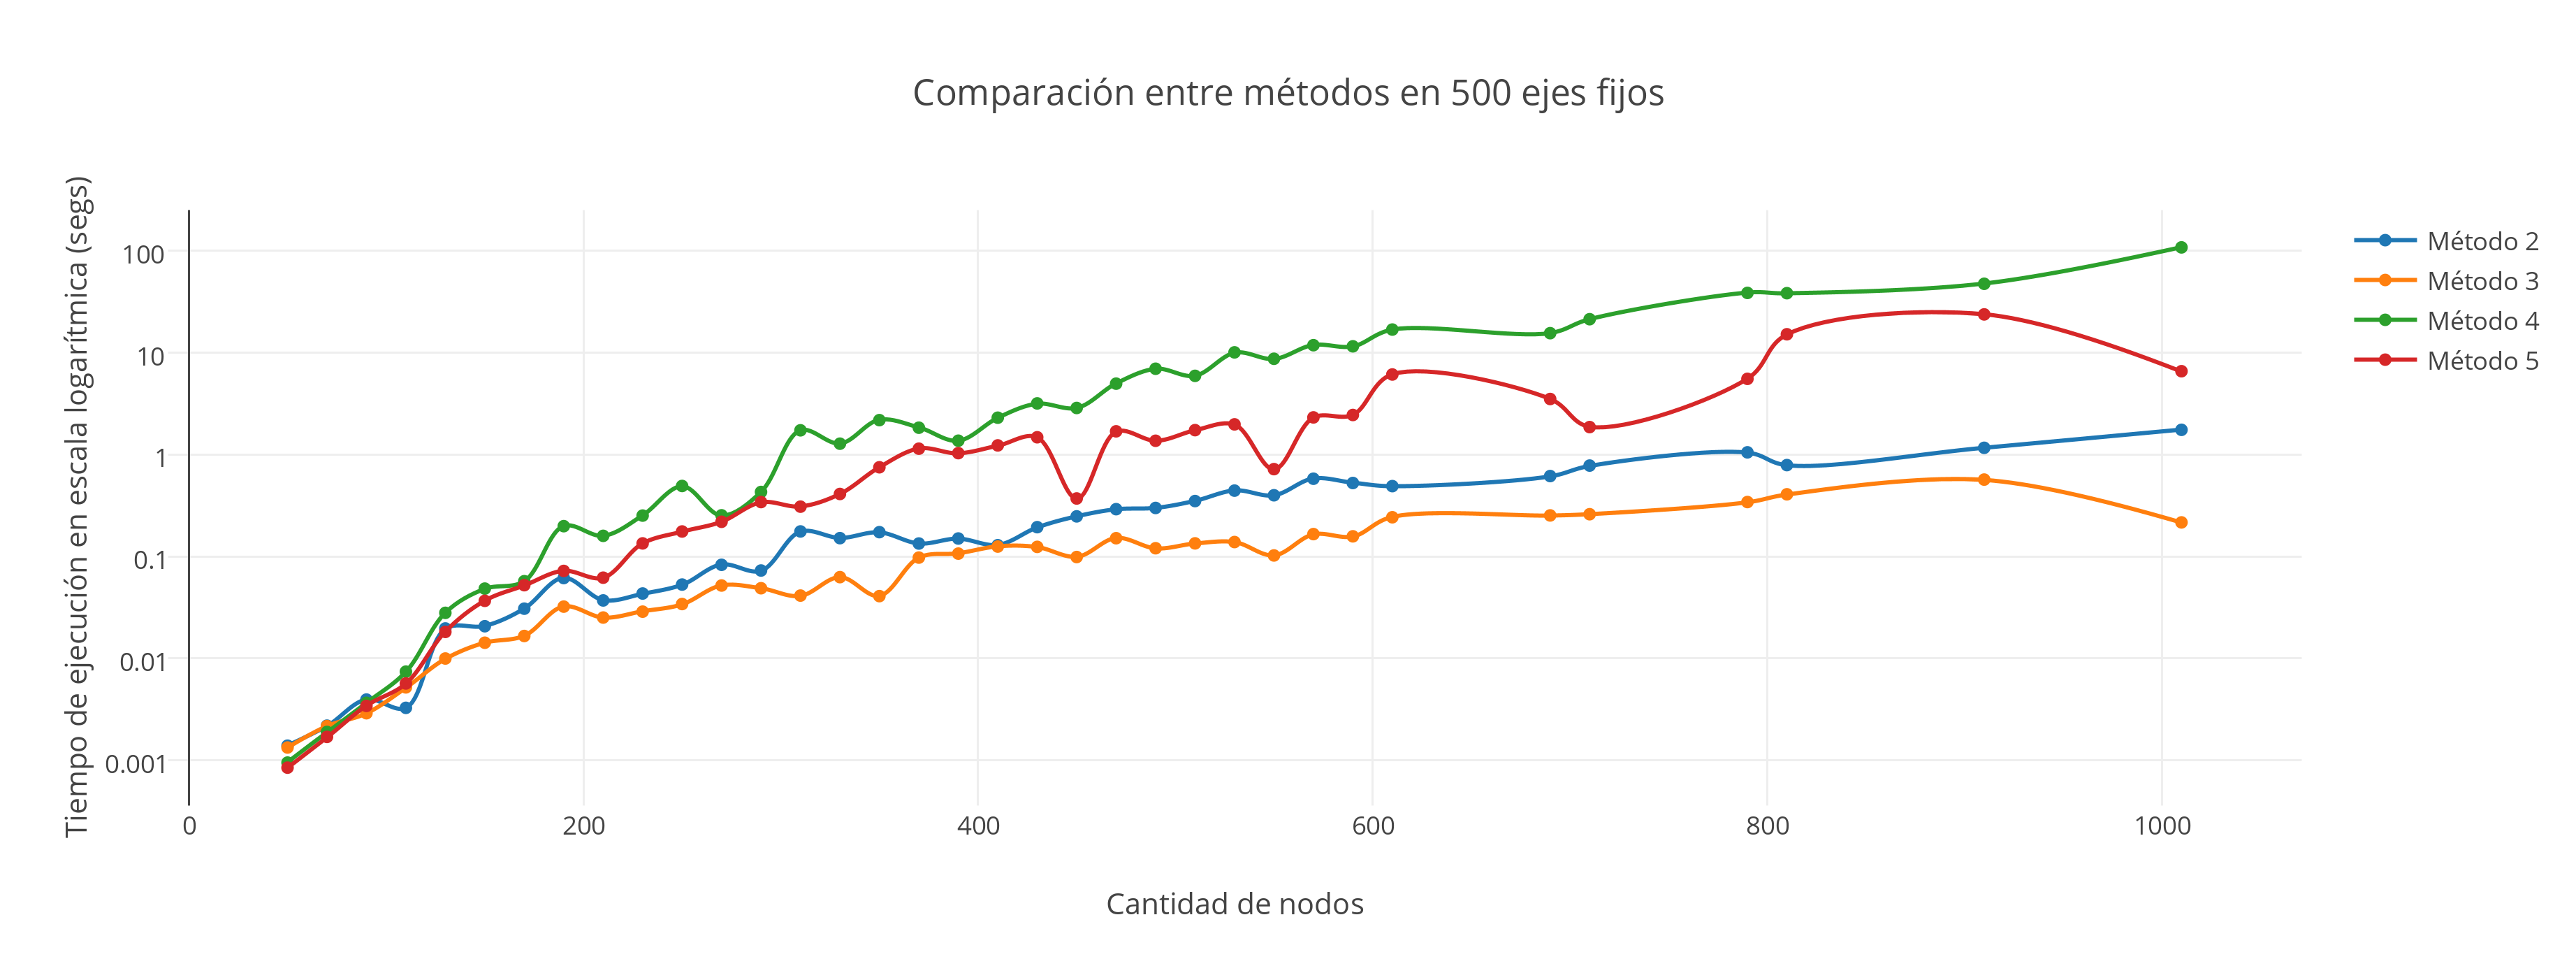
\includegraphics[scale=0.55]{imagenes/local/tiempos/500ejes.png}
% 	\caption{}
%	\label{10Nodos}
   \end{center}
 \end{figure}
 
   \begin{figure}[h!]
   \begin{center}
 	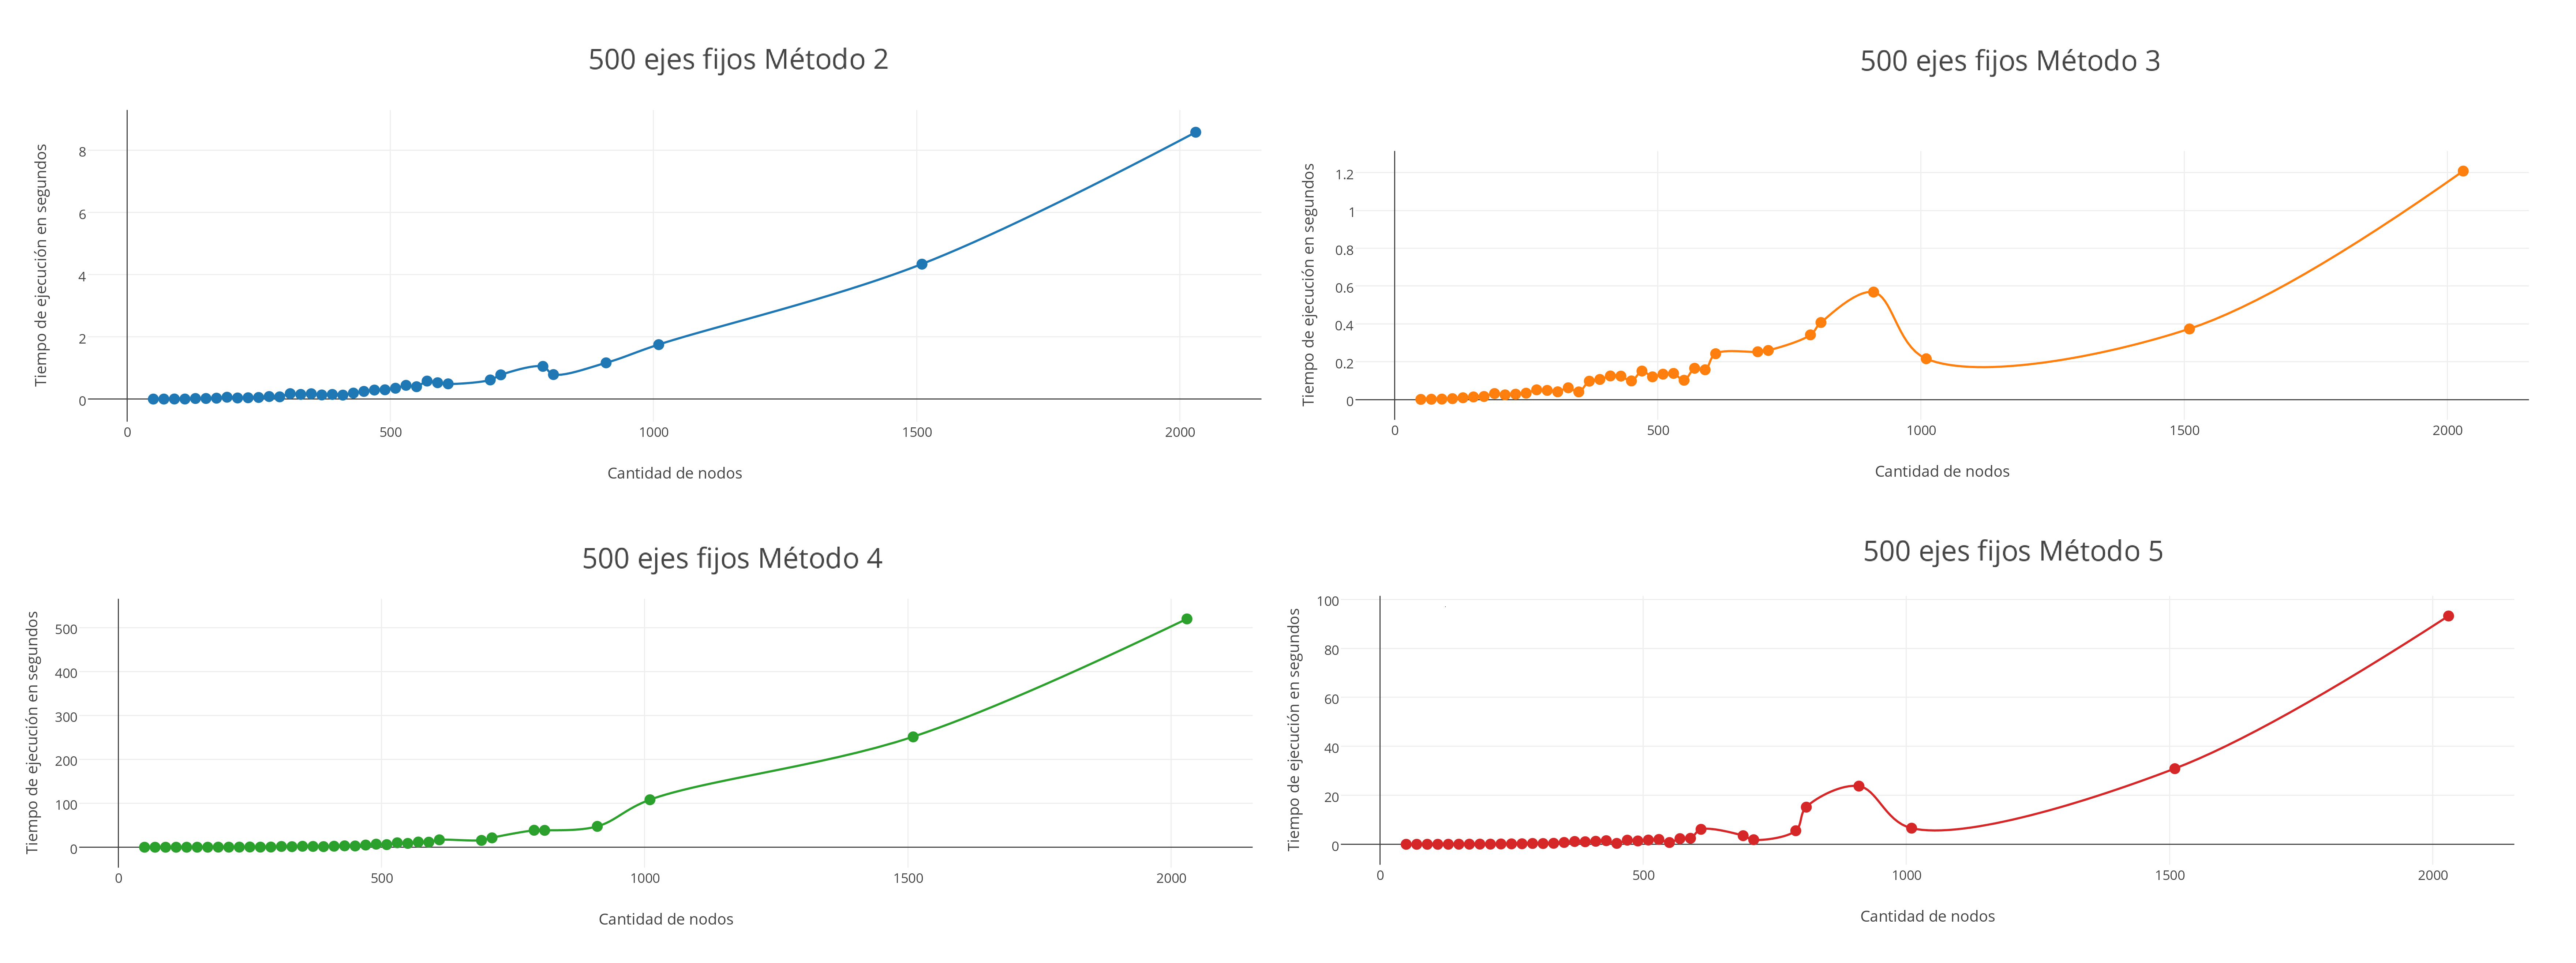
\includegraphics[scale=0.08]{imagenes/local/tiempos/500ejes2.png}
% 	\caption{}
%	\label{10Nodos}
   \end{center}
 \end{figure}

Al realizar el mismo procedimiento pero ahora con 500 ejes fijos lo que se puede apreciar es que, si bien los m\'etodos 3 y 4 se mantienen en las mediciones de tiempos mayores, la curva del \textbf{M\'etodo 4} se aleja notablemente de los dem\'as.\\

En las ampliaciones de los m\'etodos, desde una perspectiva amplia, se puede notar que poseen un comportamiento que asimila \textcolor{red}{polinomial} al igual que en el caso anterior. Se podr\'ia decir que la causa de que las gr\'aficas no sean estr\'ictamente creciente se debe a la complejidad $O(n^5)$ y $O(n^6)$.

\newpage

   \begin{figure}[h!]
   \begin{center}
 	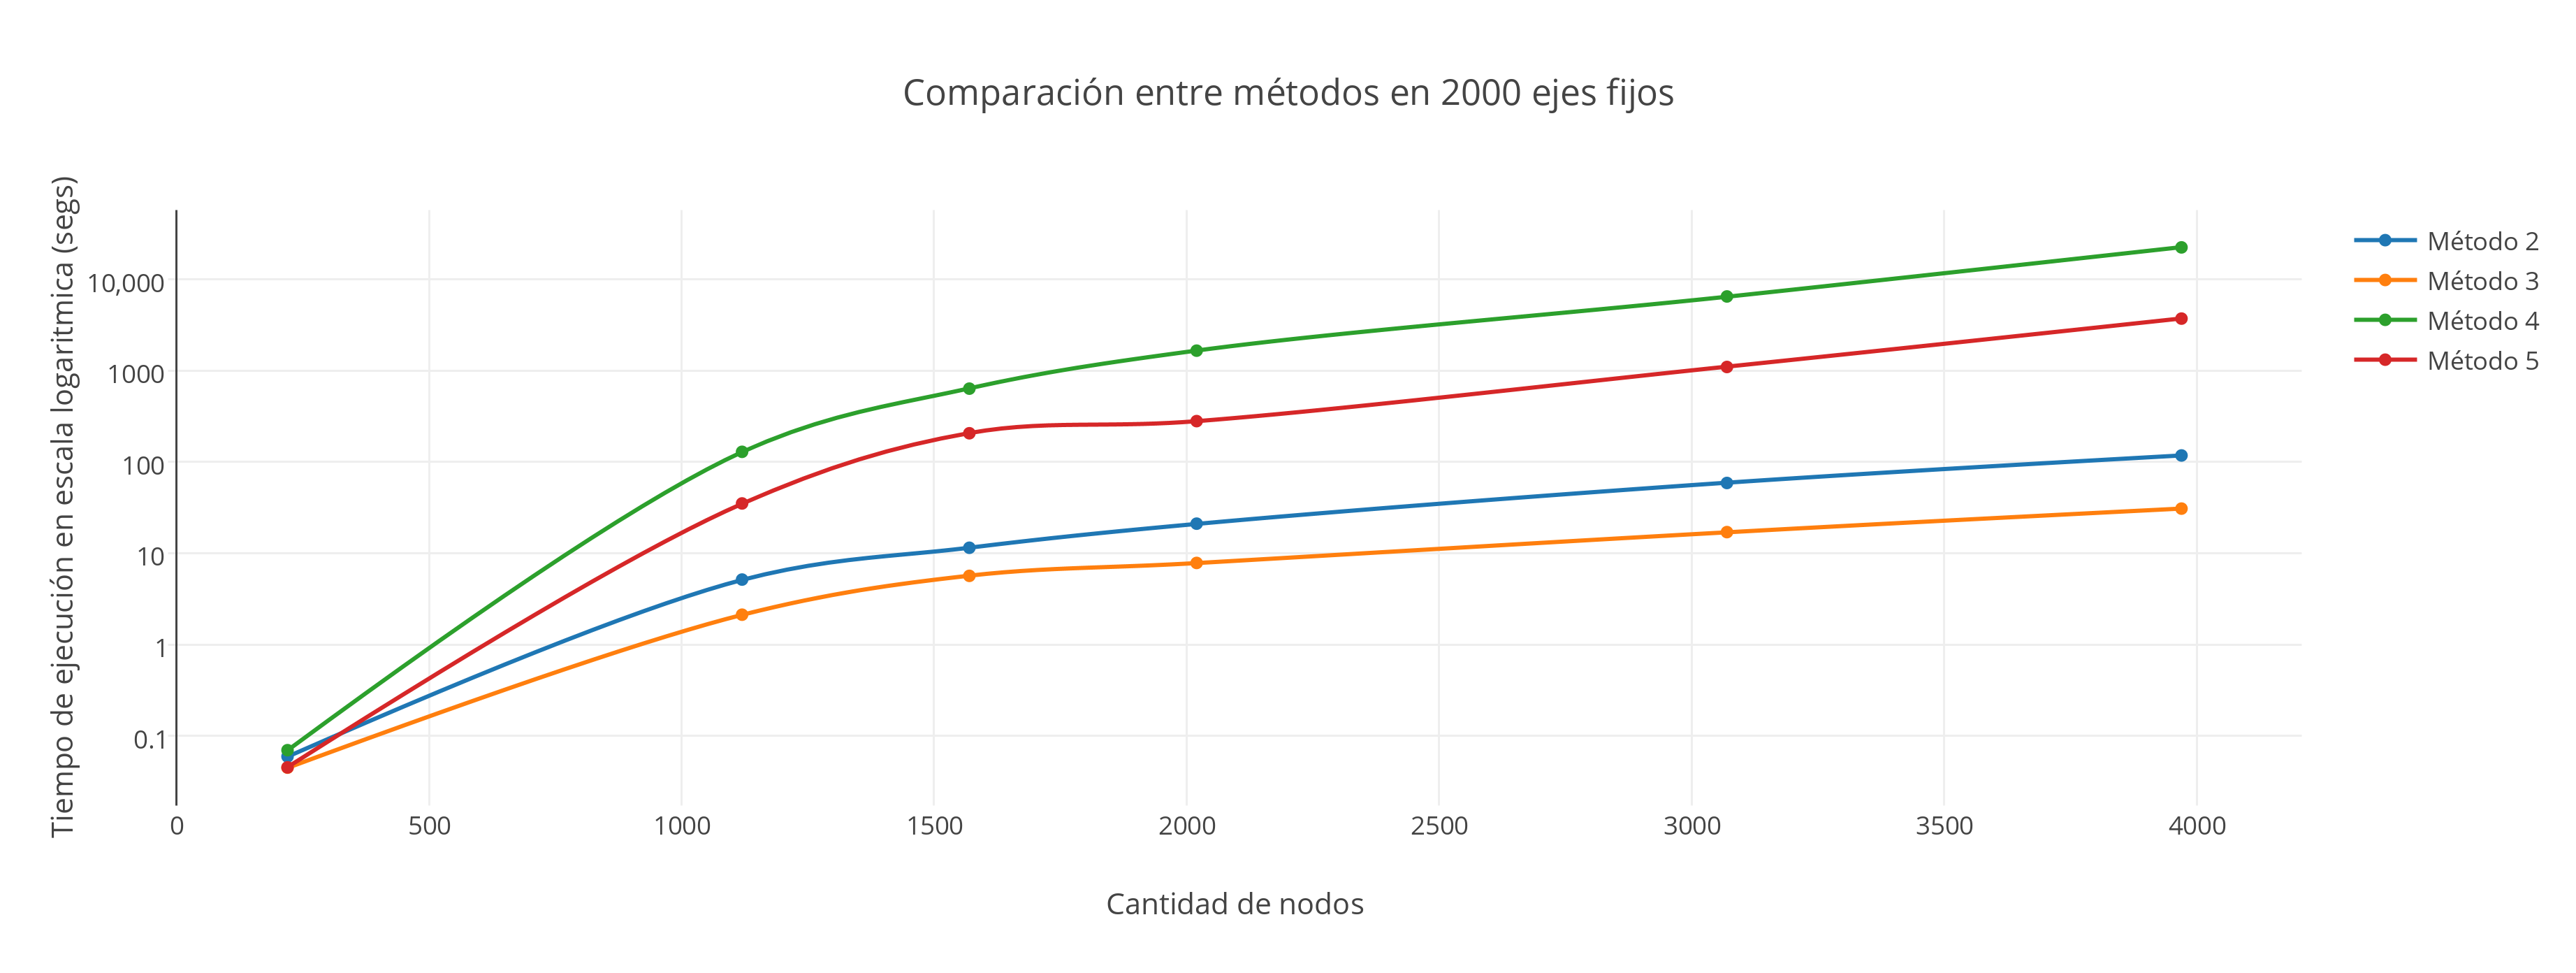
\includegraphics[scale=0.55]{imagenes/local/tiempos/2000ejes.png}
% 	\caption{}
%	\label{10Nodos}
   \end{center}
 \end{figure}
 
  \begin{figure}[h!]
   \begin{center}
 	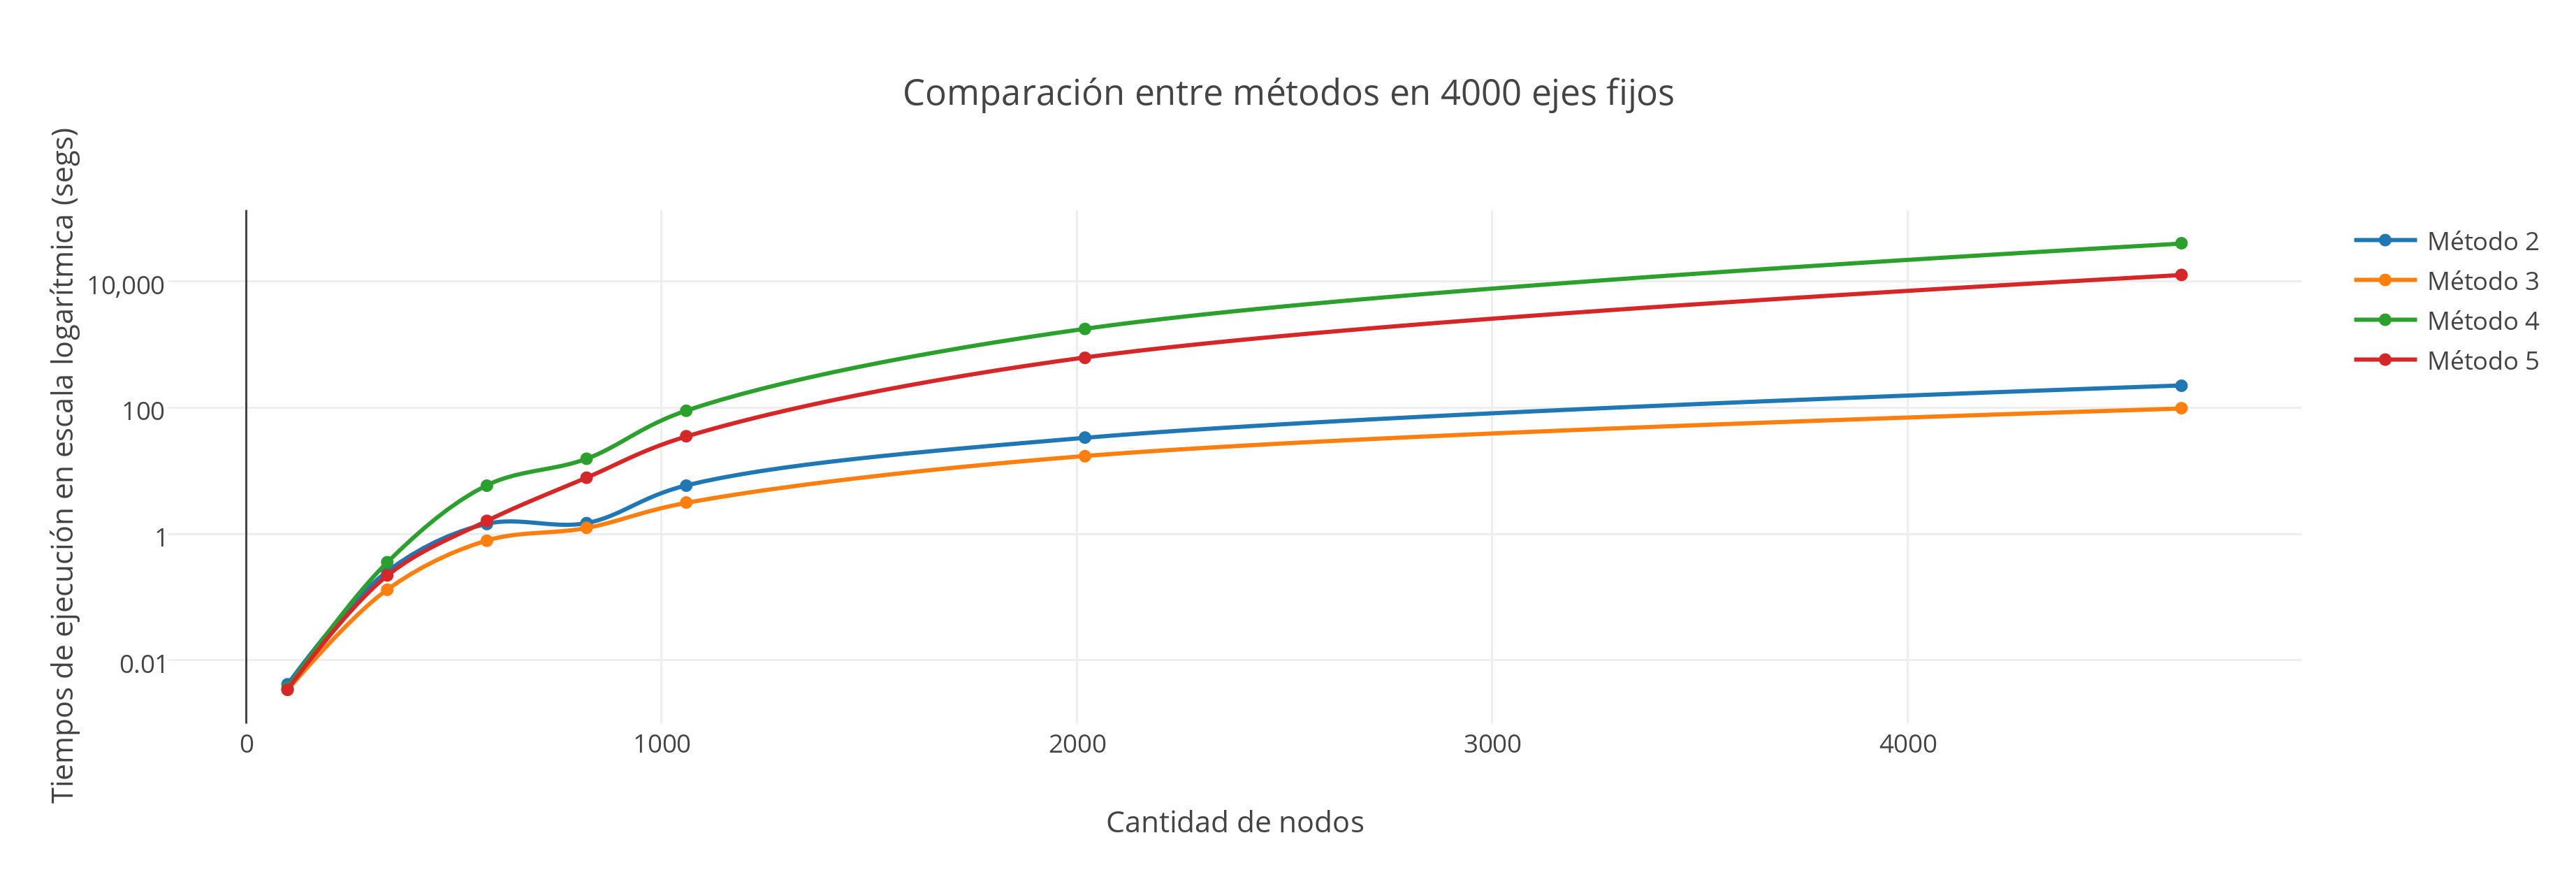
\includegraphics[scale=0.55]{imagenes/local/tiempos/4000ejes.png}
% 	\caption{}
%	\label{10Nodos}
   \end{center}
 \end{figure}
  
Al plantear la misma experimentaci\'on con cantidad de ejes mayor, se puede apreciar un comportamiento an\'alogo donde el \textbf{m\'etodo 4} posee un tiempo de ejecuci\'on notablemente mayor al resto y el \textbf{m\'etodo 3} permanece siendo el de menor tiempo de ejecuci\'on.  
  
 \newpage  
  
\subsubsection*{Nodos Fijos}

En esta instancia, se contrastar\'an grupos de grafos que posean cantidad de nodos fijos: 200, 300, 500, 600 y 700 variando en cada caso la cantidad de ejes. Se comparan los tiempos de ejecuci\'on entre los cuatro m\'etodos planteados en los casos generados. 

  \begin{figure}[h!]
   \begin{center}
 	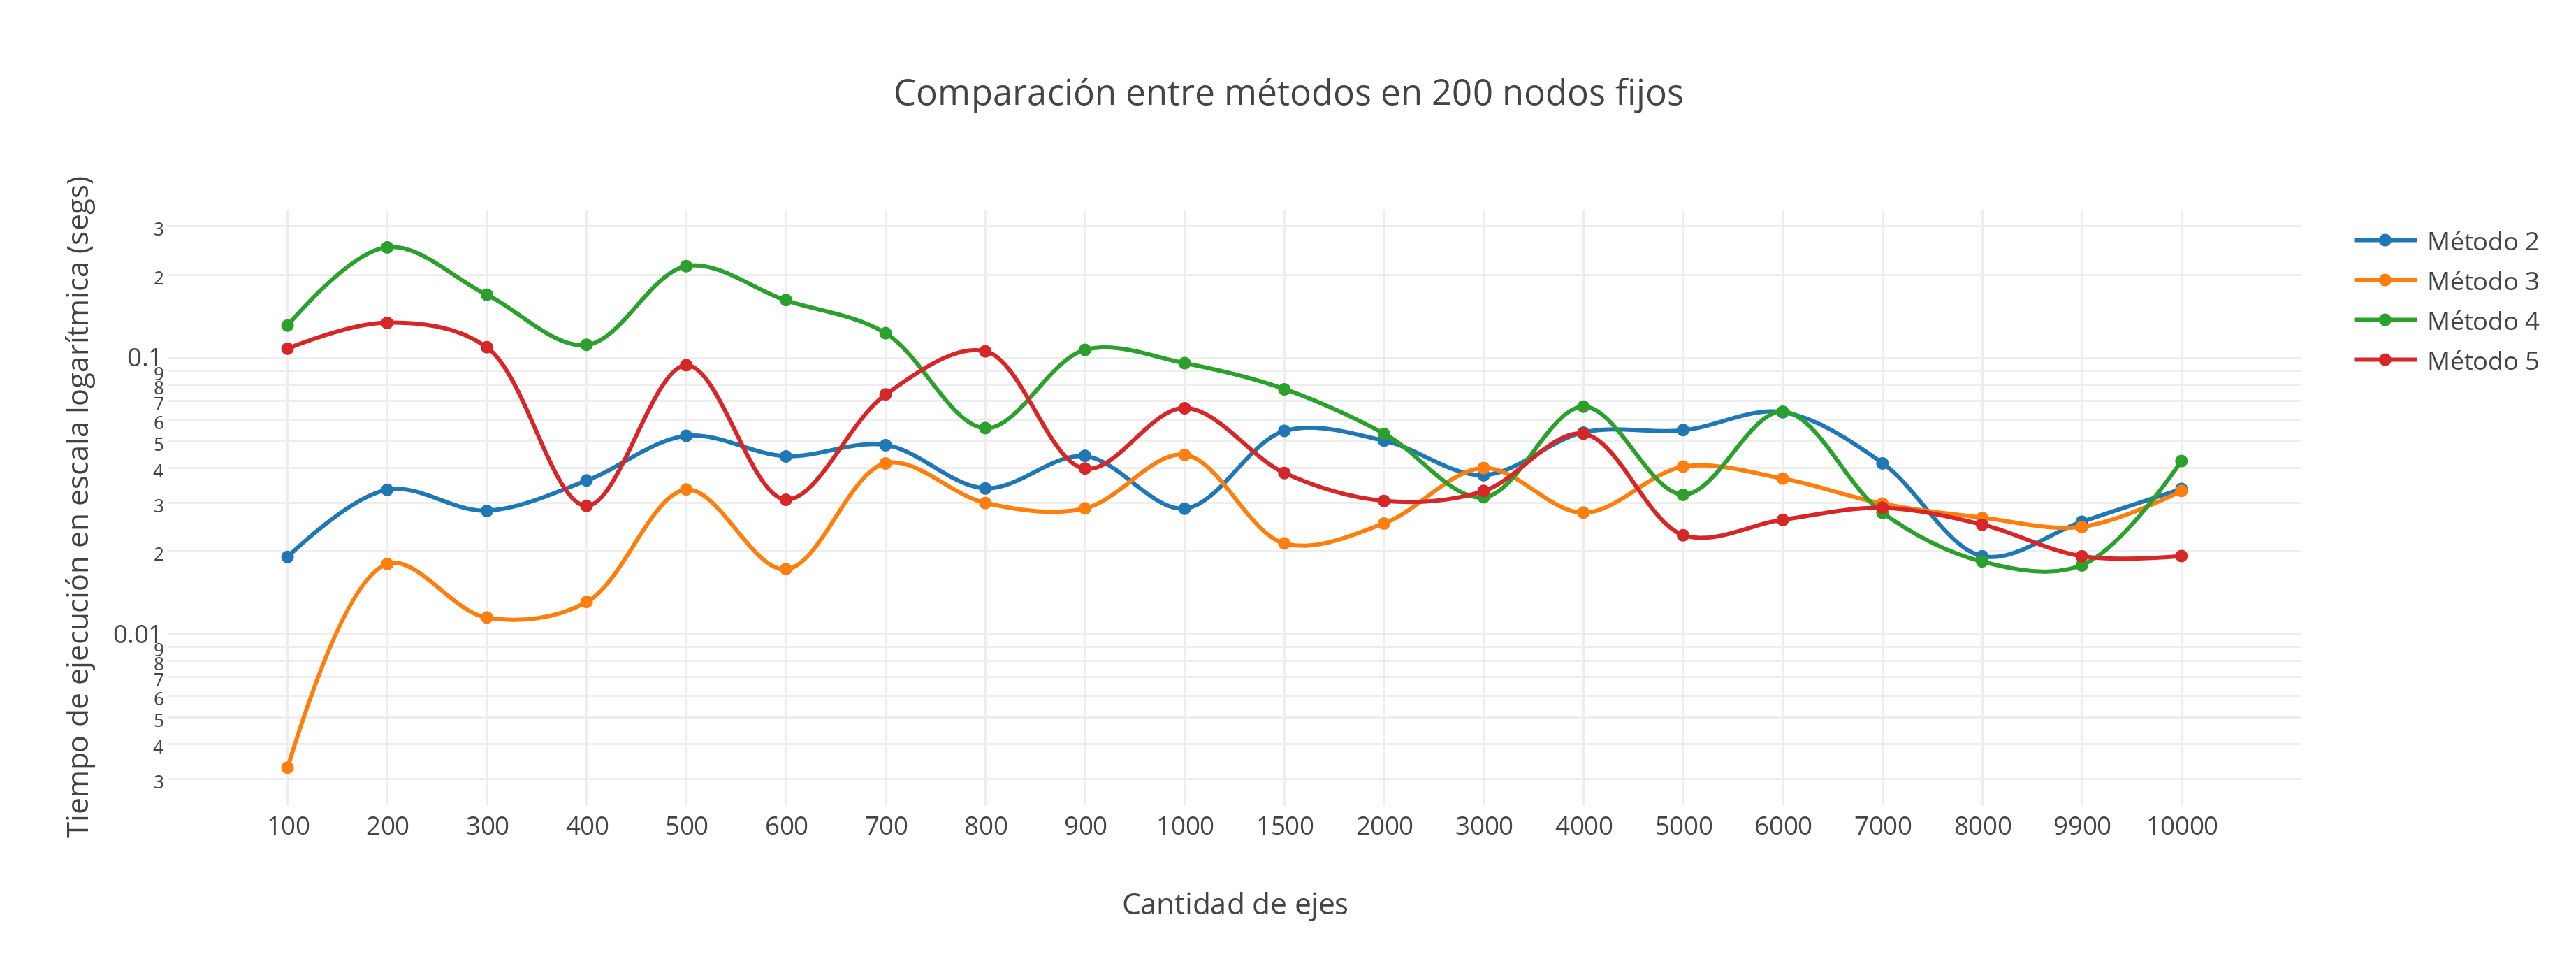
\includegraphics[scale=0.55]{imagenes/local/tiempos/200nodos.png}
% 	\caption{}
%	\label{10Nodos}
   \end{center}
 \end{figure}
 
Dando una observaci\'on general sobre este gr\'afico, se puede apreciar que para todos los m\'etodos el tiempo de ejecuci\'on disminuye al aumentar la cantidad de ejes. \\

A simple vista podr\'ia sonar un poco absurdo, sin embargo la causa de este comportamiento  est\'a ligada a que al existir mayor cantidad de ejes (manteniendo la cantidad de nodos) aumenta el grado de los nodos. Por lo tanto\textcolor{red}{, al igual que el algoritmo Goloso(?), } cuando se arma una soluci\'on inicial se inserta el nodo de mayor grado. Luego, se descartan todos los nodos vecinos ya que no ser\'an candidatos al conjunto soluci\'on.

Si bien, para descartar nodos vecinos, se debe recorrer la lista de adyacencia completa; ese tiempo es compensado al tener menos nodos en la siguiente iteraci\'on para recorrer.\\

En cuanto a la parte del algoritmo que consiste en la b\'usqueda local, \textcolor{red}{Completar algo aca...}

   \begin{figure}[h!]
   \begin{center}
 	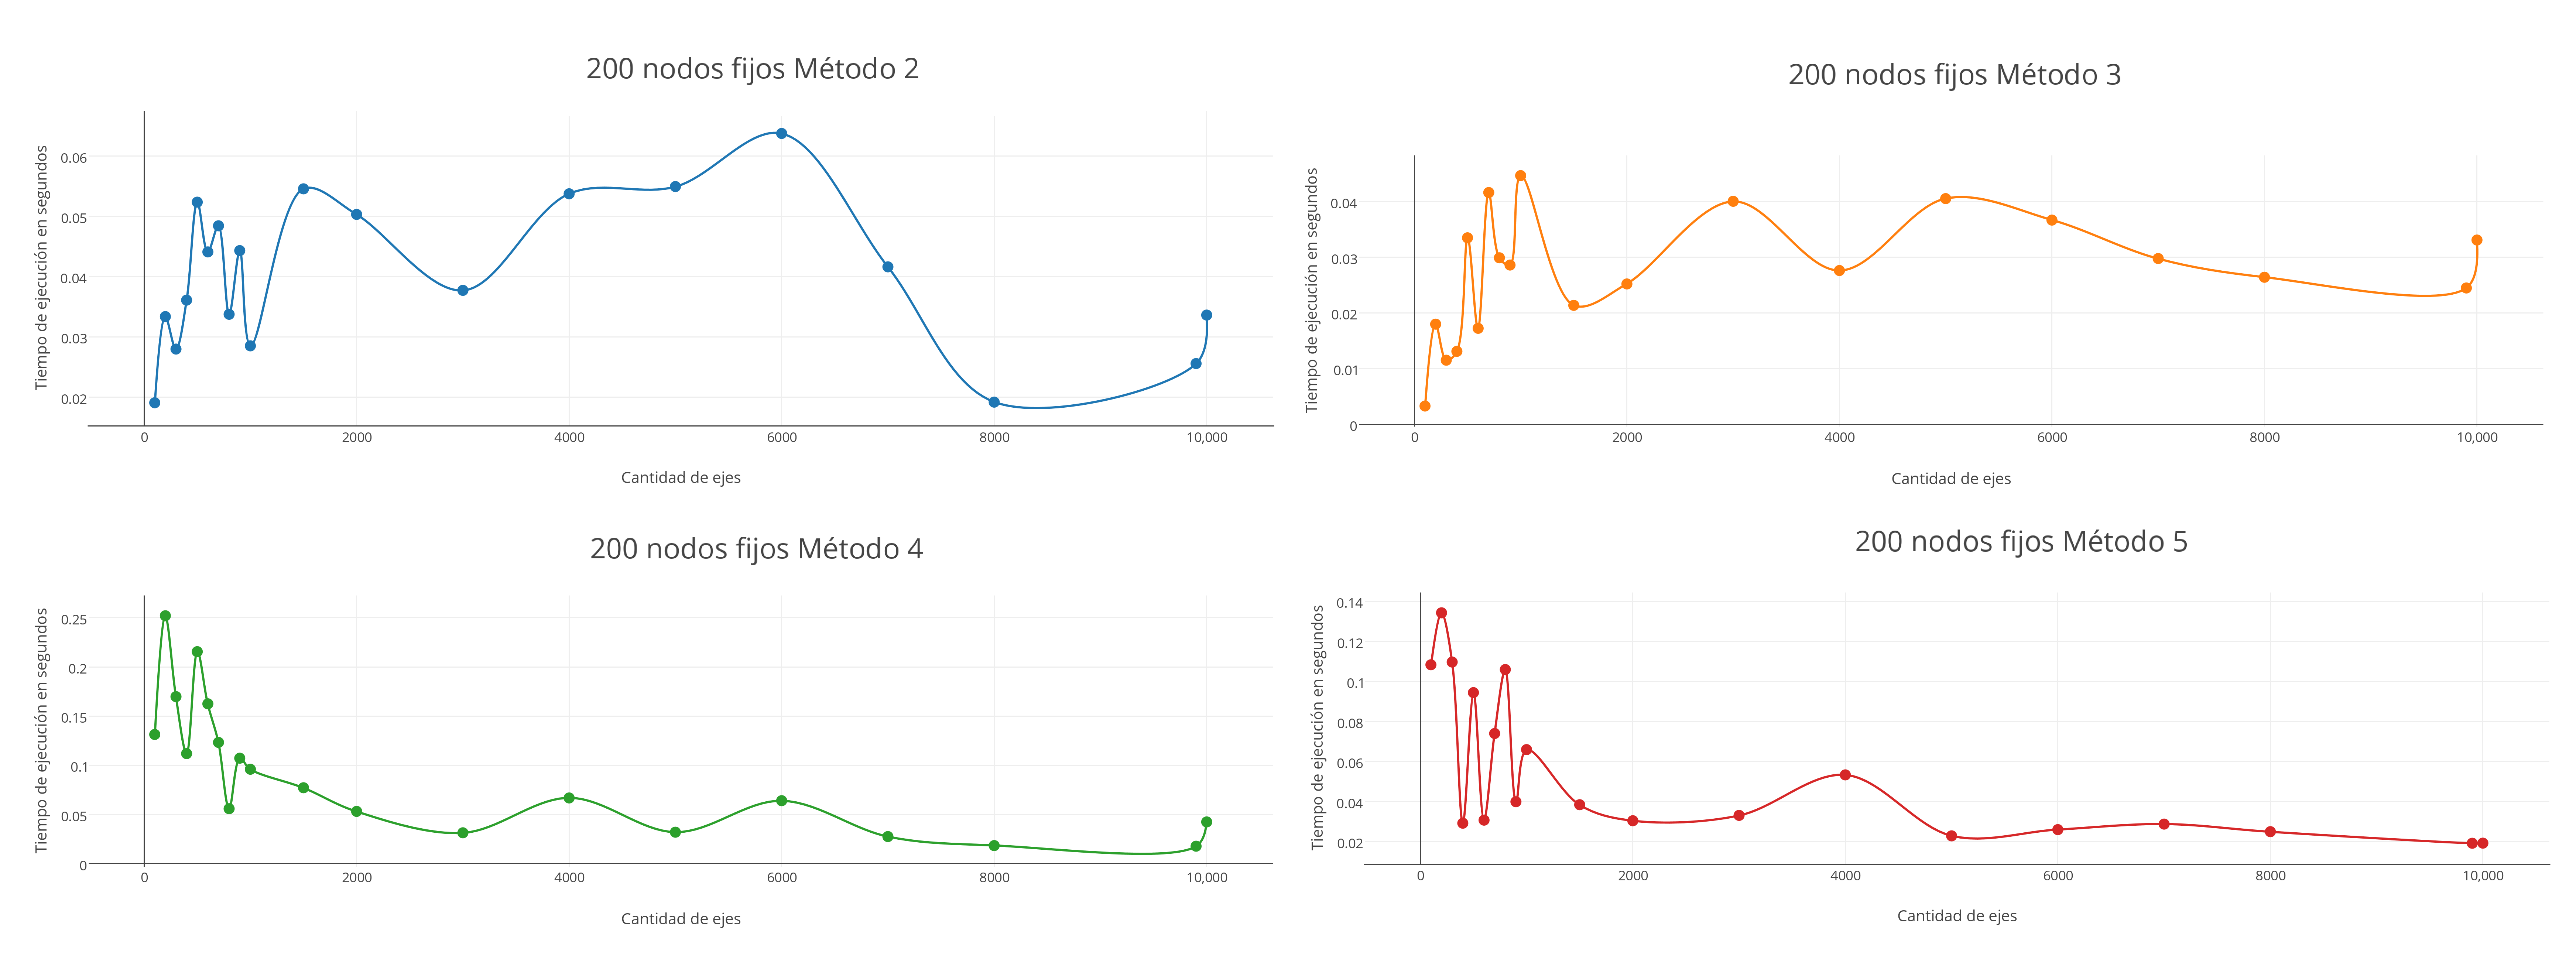
\includegraphics[scale=0.08]{imagenes/local/tiempos/200nodos2.png}
% 	\caption{}
%	\label{10Nodos}
   \end{center}
 \end{figure}
 
 Haciendo hincapie en cada m\'etodo por separado, se observa un comportamiento distinguible.\\
 
 Si bien las curvas de los cuatro m\'etodos oscilan notablemente, si uno observa bajo un punto de vista general se puede apreciar que los m\'etodos 4 y 5 tienen un comportamiento notablemente decreciente similar al de una curva \textcolor{red}{polinomial (?}. Ambos m\'etodos utilizan la segunda vecindad, lo que indicar\'ia que el comportamiento es causado por \textcolor{red}{completar!!!}.\\
 
 Por otro lado, los m\'etodos 3 y 4 poseen un crecimiento abrupto con una cantidad de ejes menor y despu\'es sus curvas oscilan de manera, se podr\'ia decir que, constante. Como ambas manejan la misma vecindad, un potencial causante de dicho comportamiento corresponde a ... \textcolor{red}{COMPLETAR}\\

\bigskip

Ejecutamos la misma experimentaci\'on, pero en esta ocasi\'on fijando la cantidad de nodos en 300, 500 y 600. 
 
  \begin{figure}[h!]
   \begin{center}
 	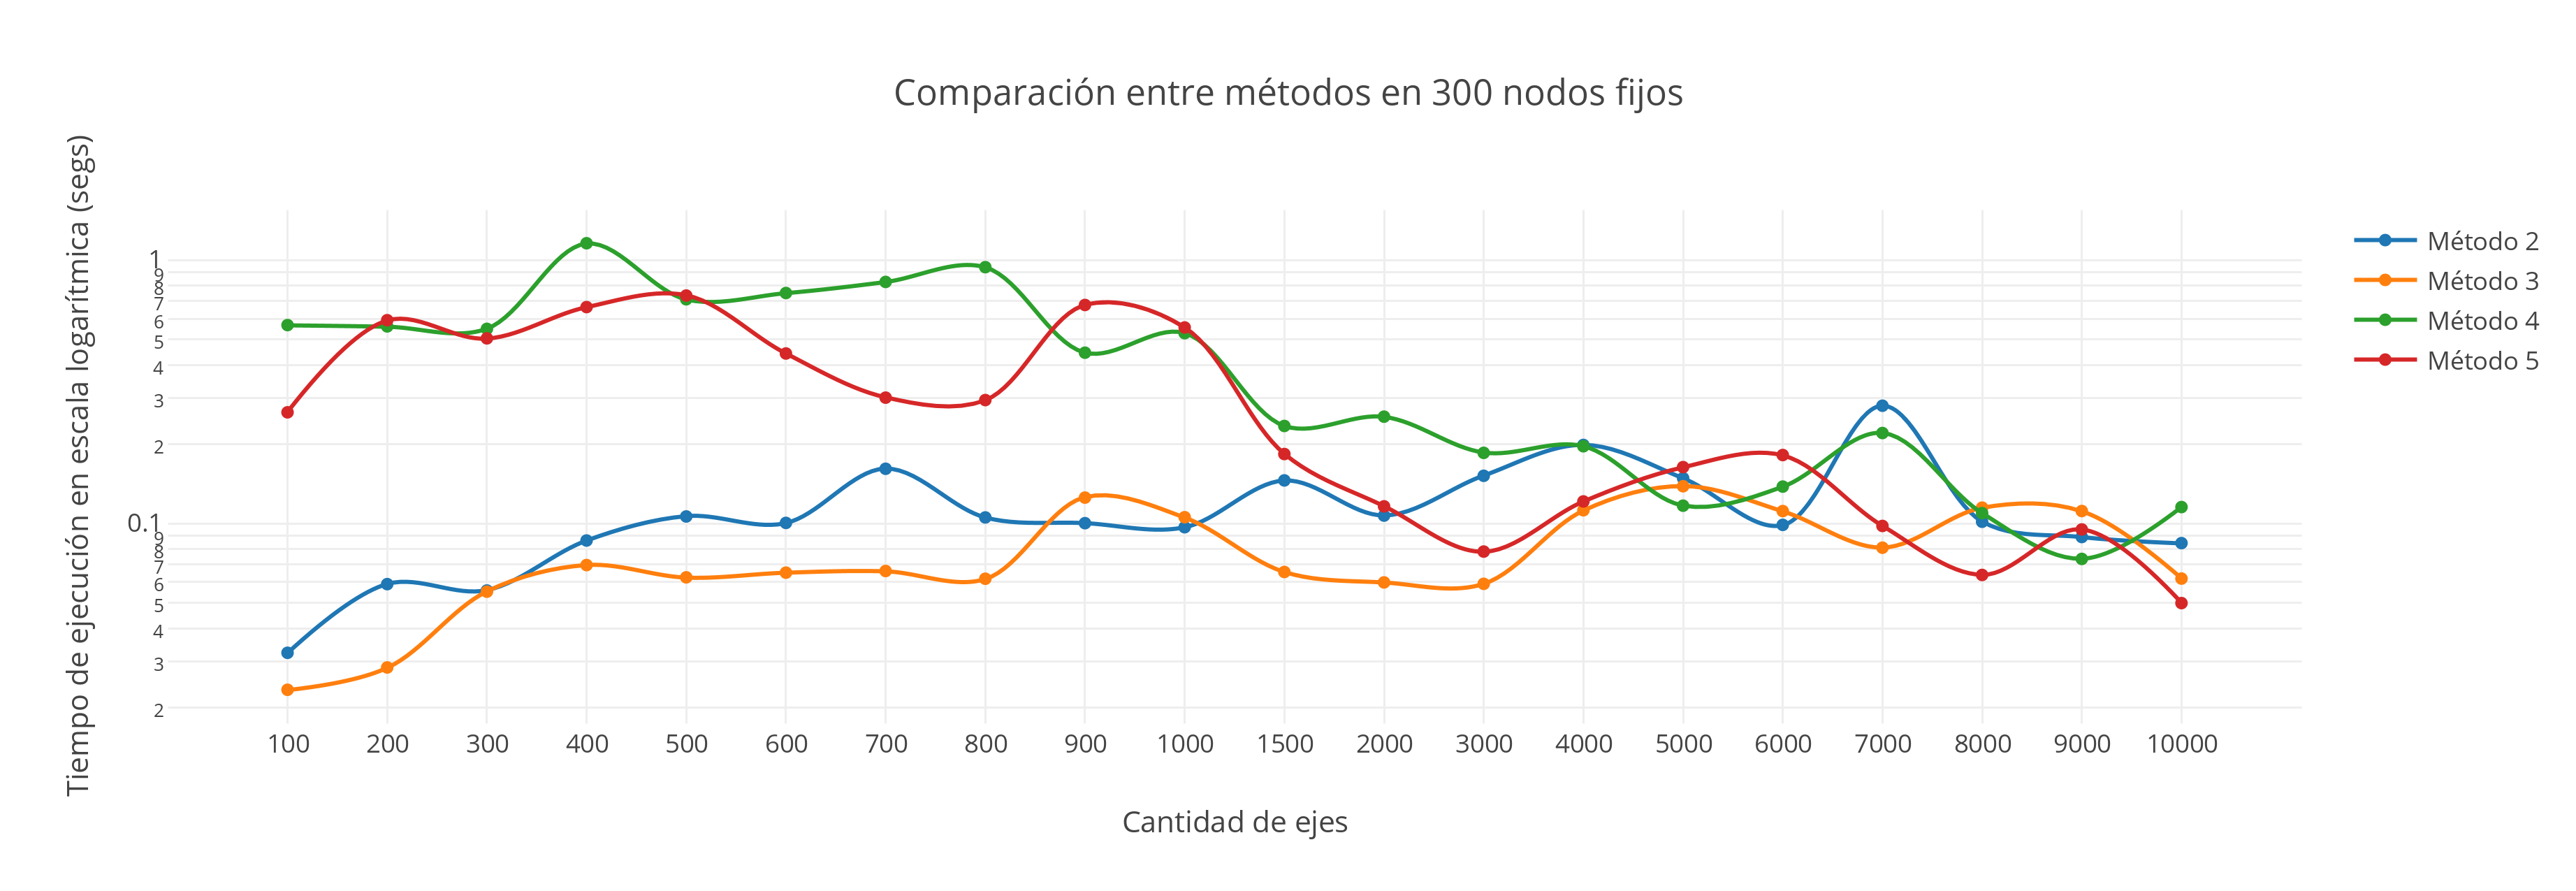
\includegraphics[scale=0.55]{imagenes/local/tiempos/300nodos.png}
% 	\caption{}
%	\label{10Nodos}
   \end{center}
 \end{figure}
 
   \begin{figure}[h!]
   \begin{center}
 	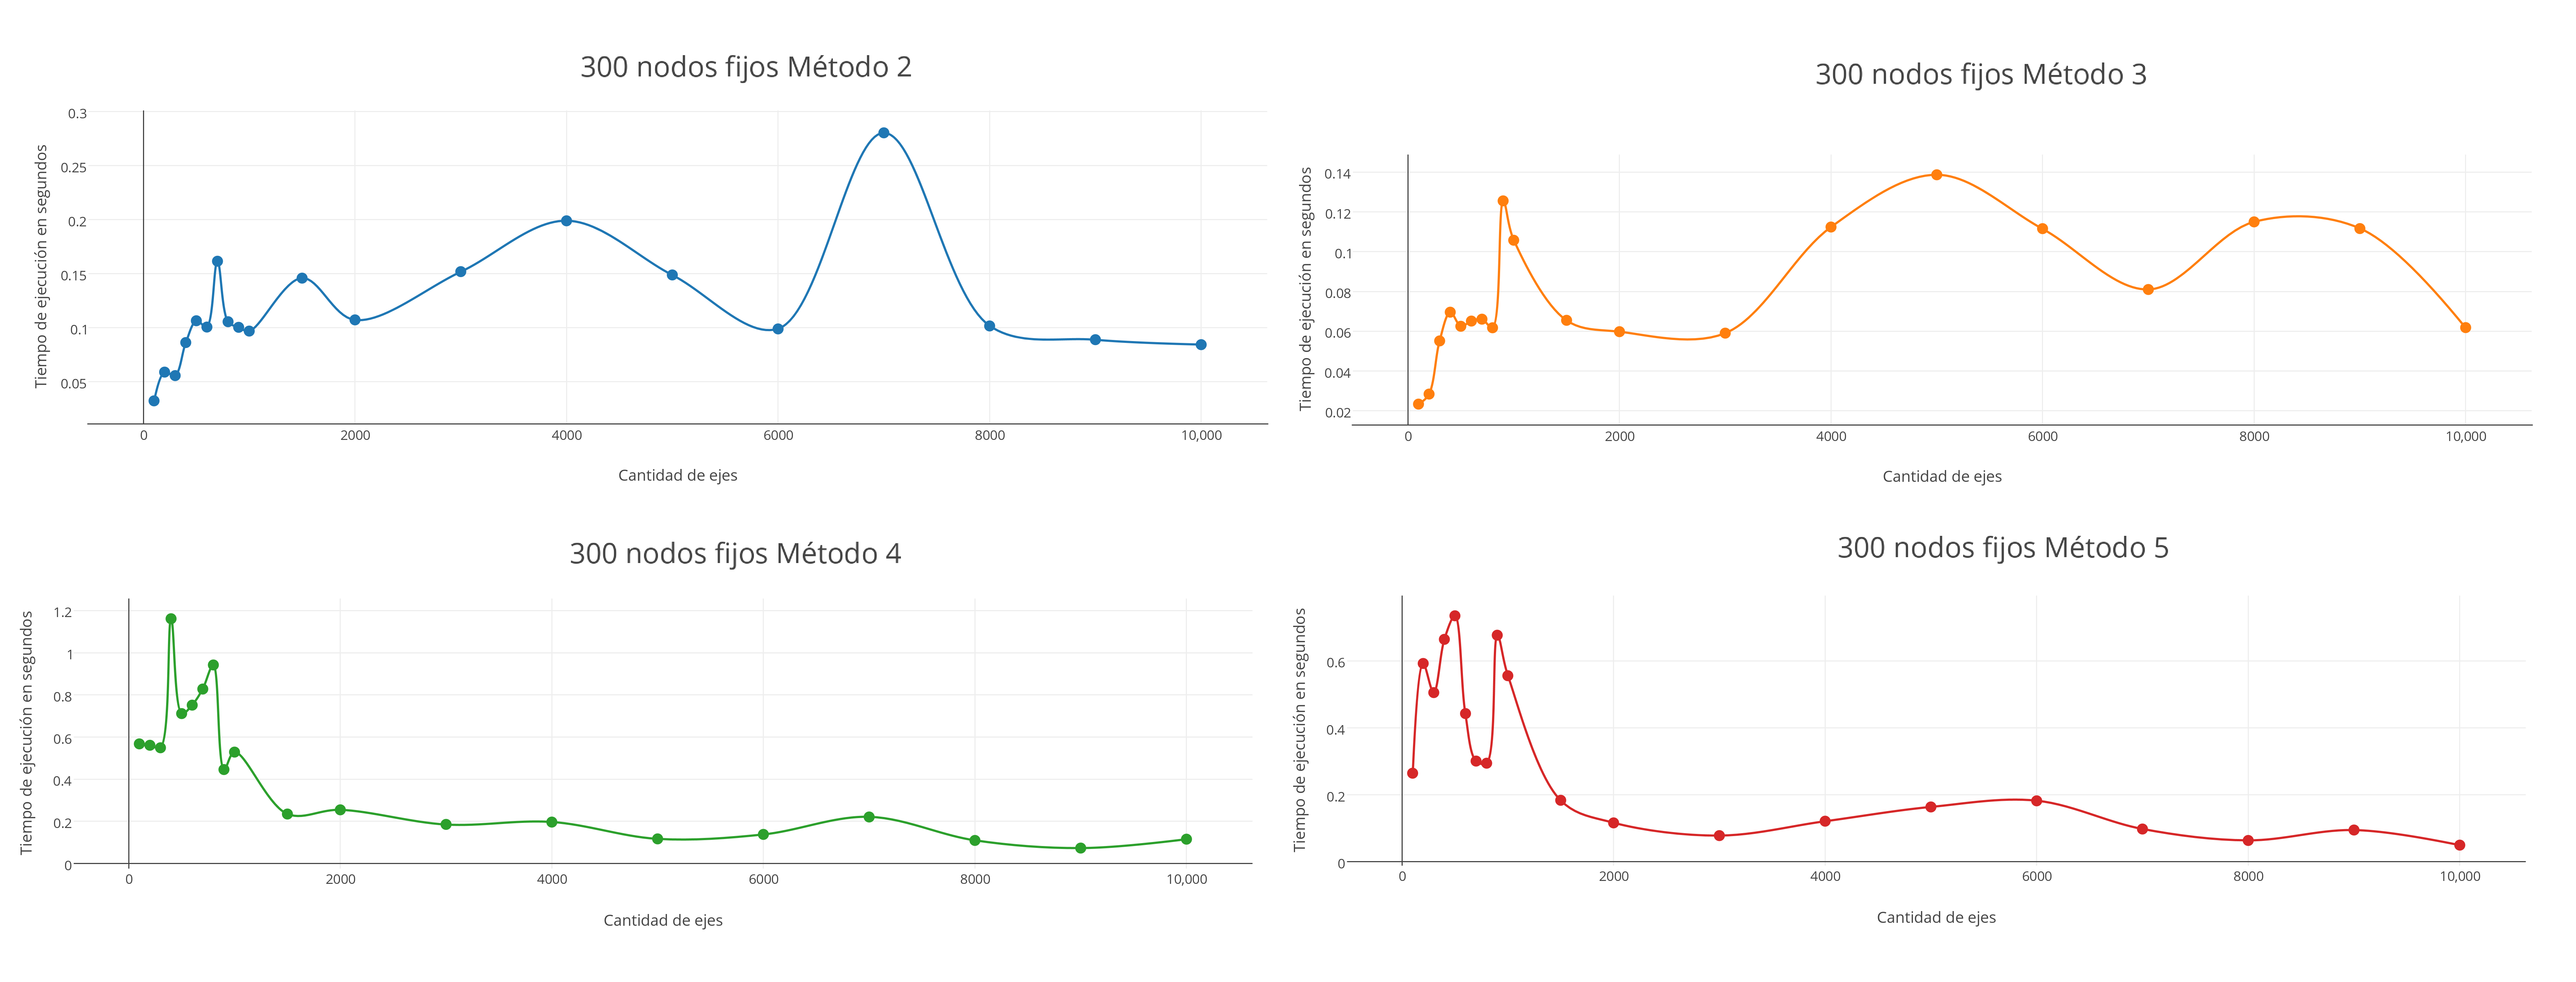
\includegraphics[scale=0.08]{imagenes/local/tiempos/300nodos2.png}
% 	\caption{}
%	\label{10Nodos}
   \end{center}
 \end{figure}



  \begin{figure}[h!]
   \begin{center}
 	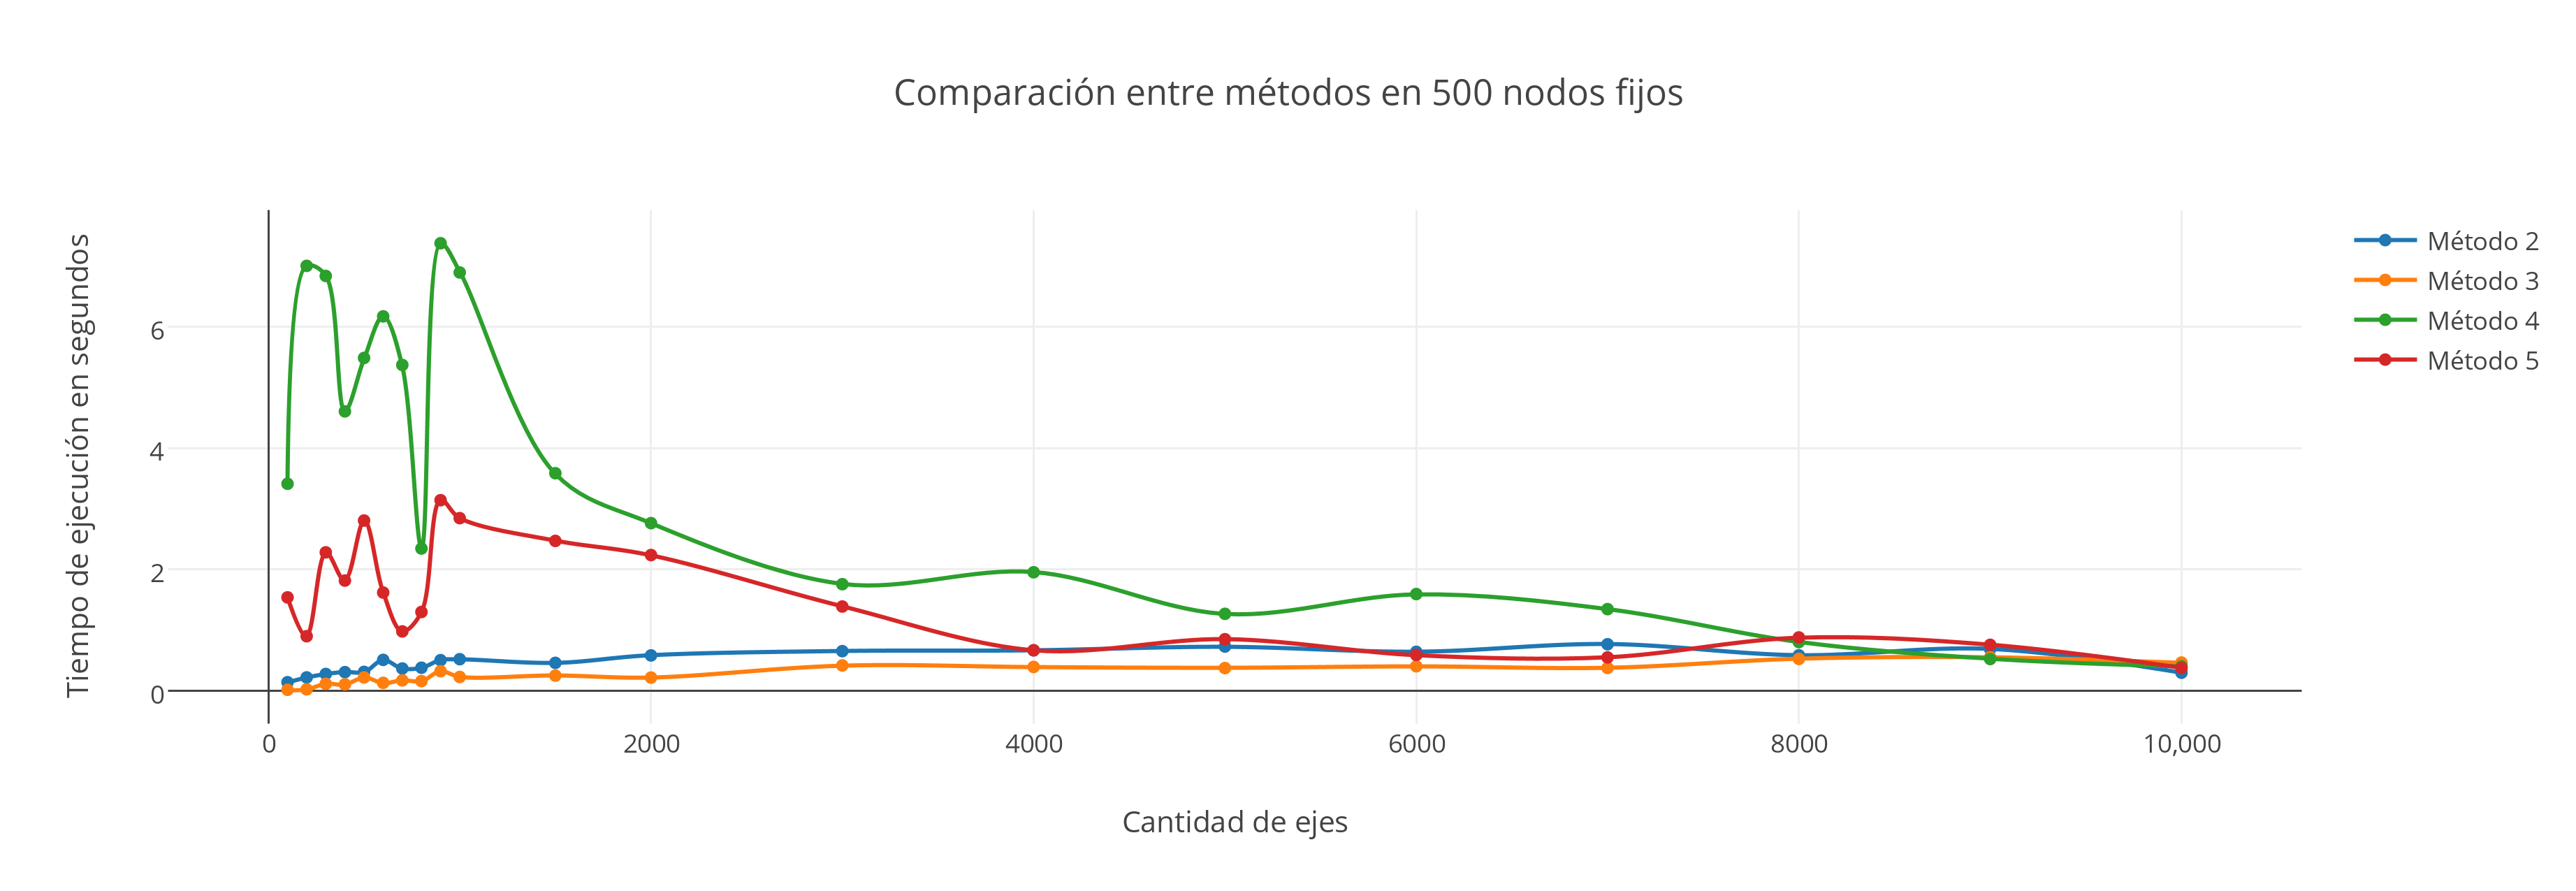
\includegraphics[scale=0.55]{imagenes/local/tiempos/500nodos.png}
% 	\caption{}
%	\label{10Nodos}
   \end{center}
 \end{figure}
 
\newpage 
 
   \begin{figure}[h!]
   \begin{center}
 	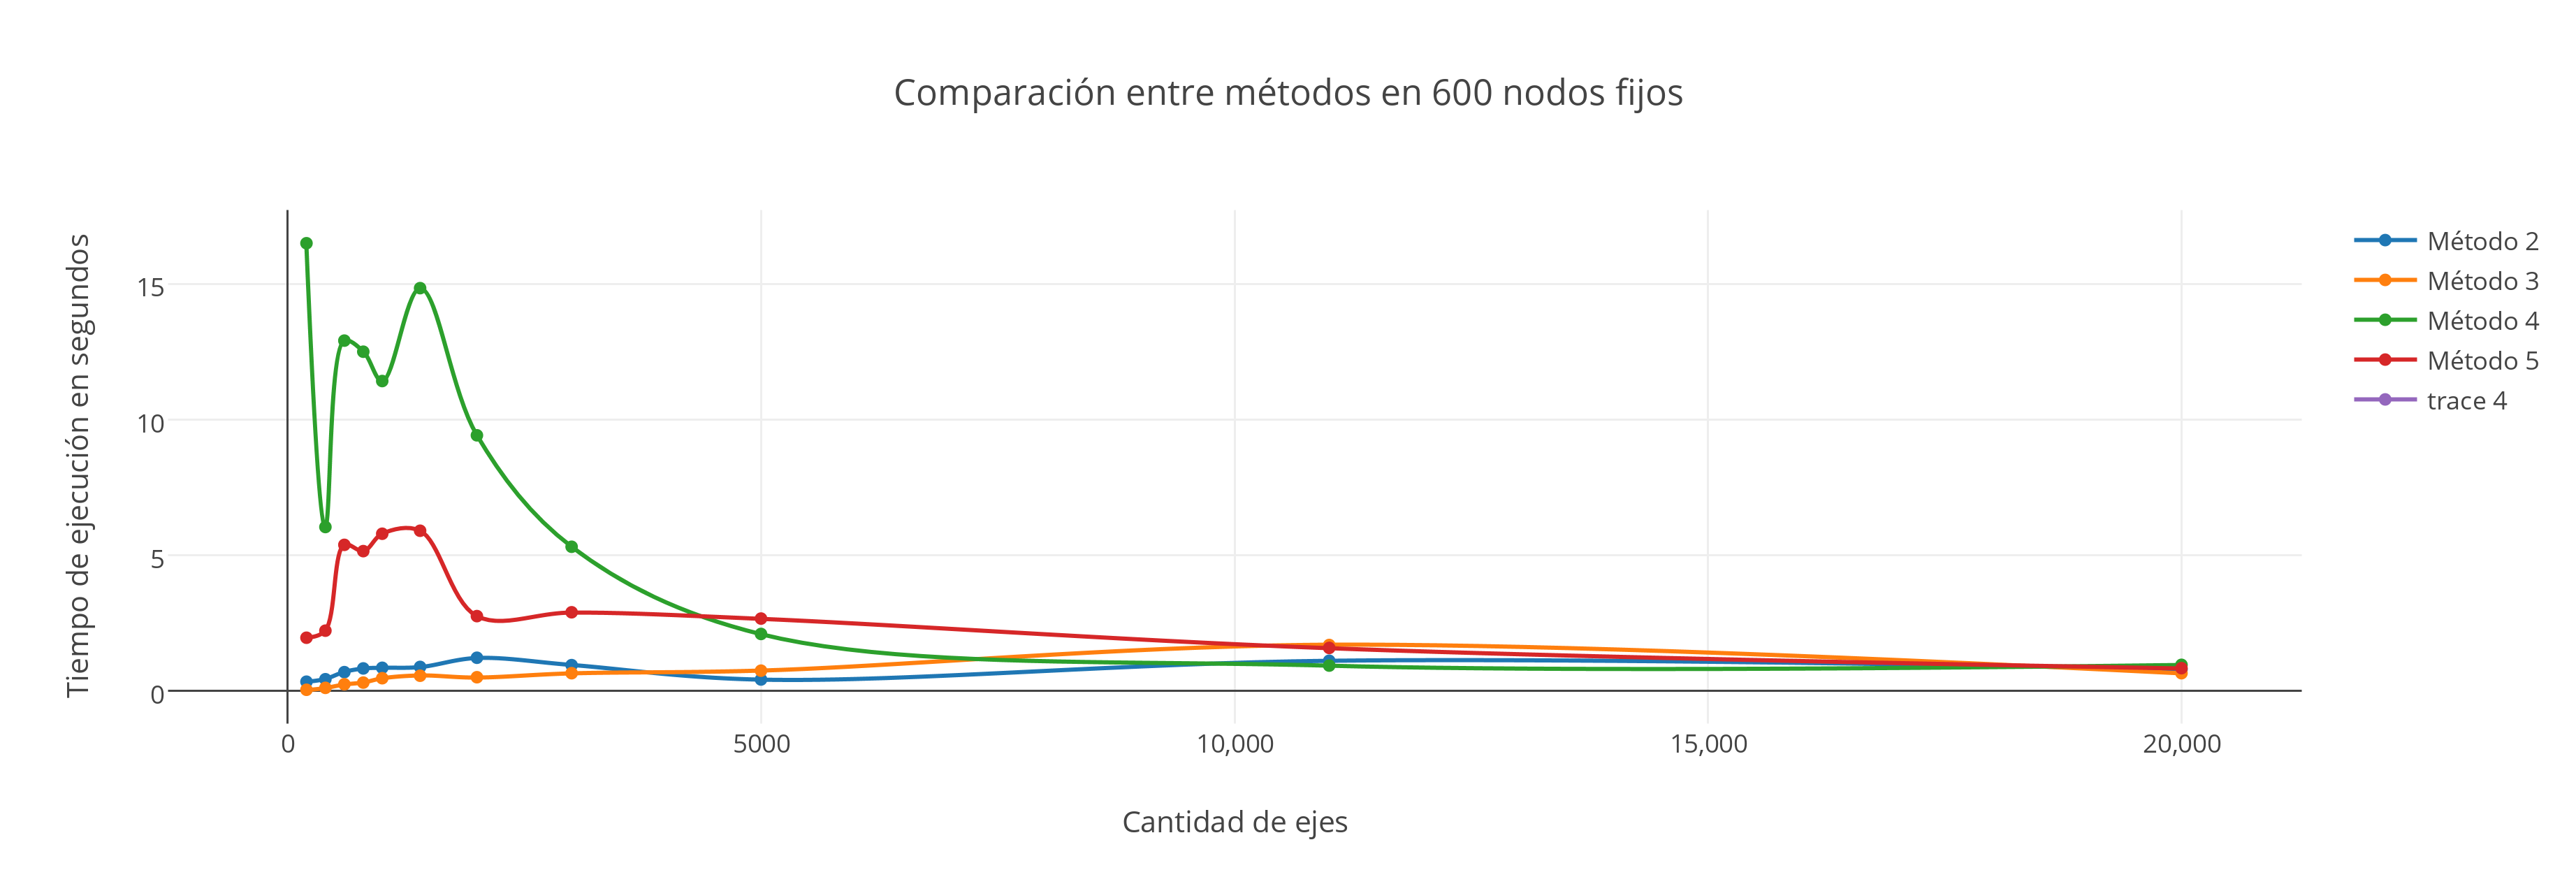
\includegraphics[scale=0.55]{imagenes/local/tiempos/600nodos.png}
% 	\caption{}
%	\label{10Nodos}
   \end{center}
 \end{figure}

La conclusi\'on que se puede sacar de este \'ultimo set de gr\'aficos es que, si se fija la cantidad de nodos, no importa en qu\'e valor, los tiempos de ejecuci\'on de los m\'etodos poseen un comportamiento similar al explicado en el inciso anterior.

Donde el \textbf{M\'etodo 4} permanece siendo quien tiene mayores tiempos de ejecuci\'on sin importar la cantidad de nodos y ejes. As\'i mismo, el \textbf{M\'etodo 3} se mantiene con los tiempos de ejecuci\'on menores.

  \begin{figure}[h!]
   \begin{center}
 	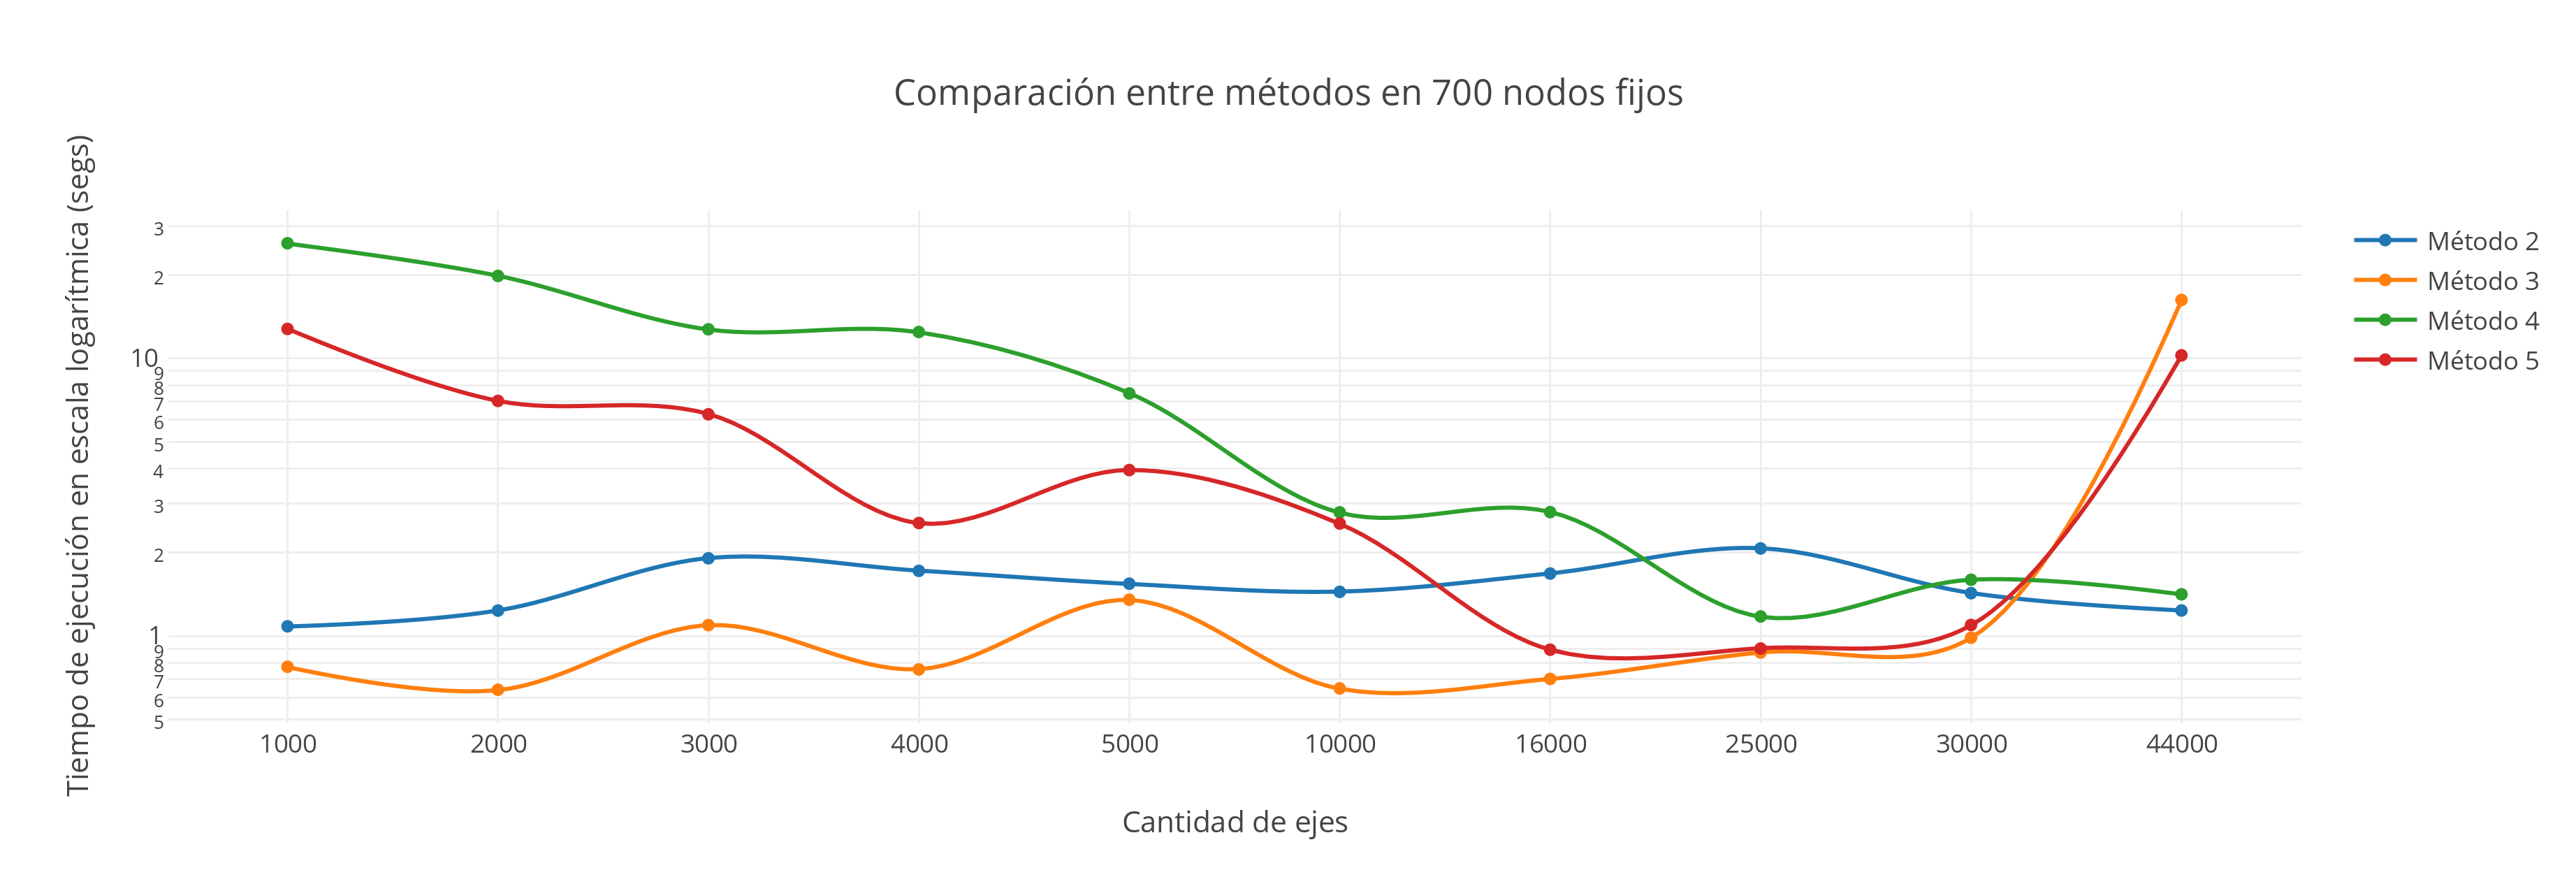
\includegraphics[scale=0.55]{imagenes/local/tiempos/700nodos.png}
% 	\caption{}
%	\label{10Nodos}
   \end{center}
 \end{figure} 
 
   \begin{figure}[h!]
   \begin{center}
 	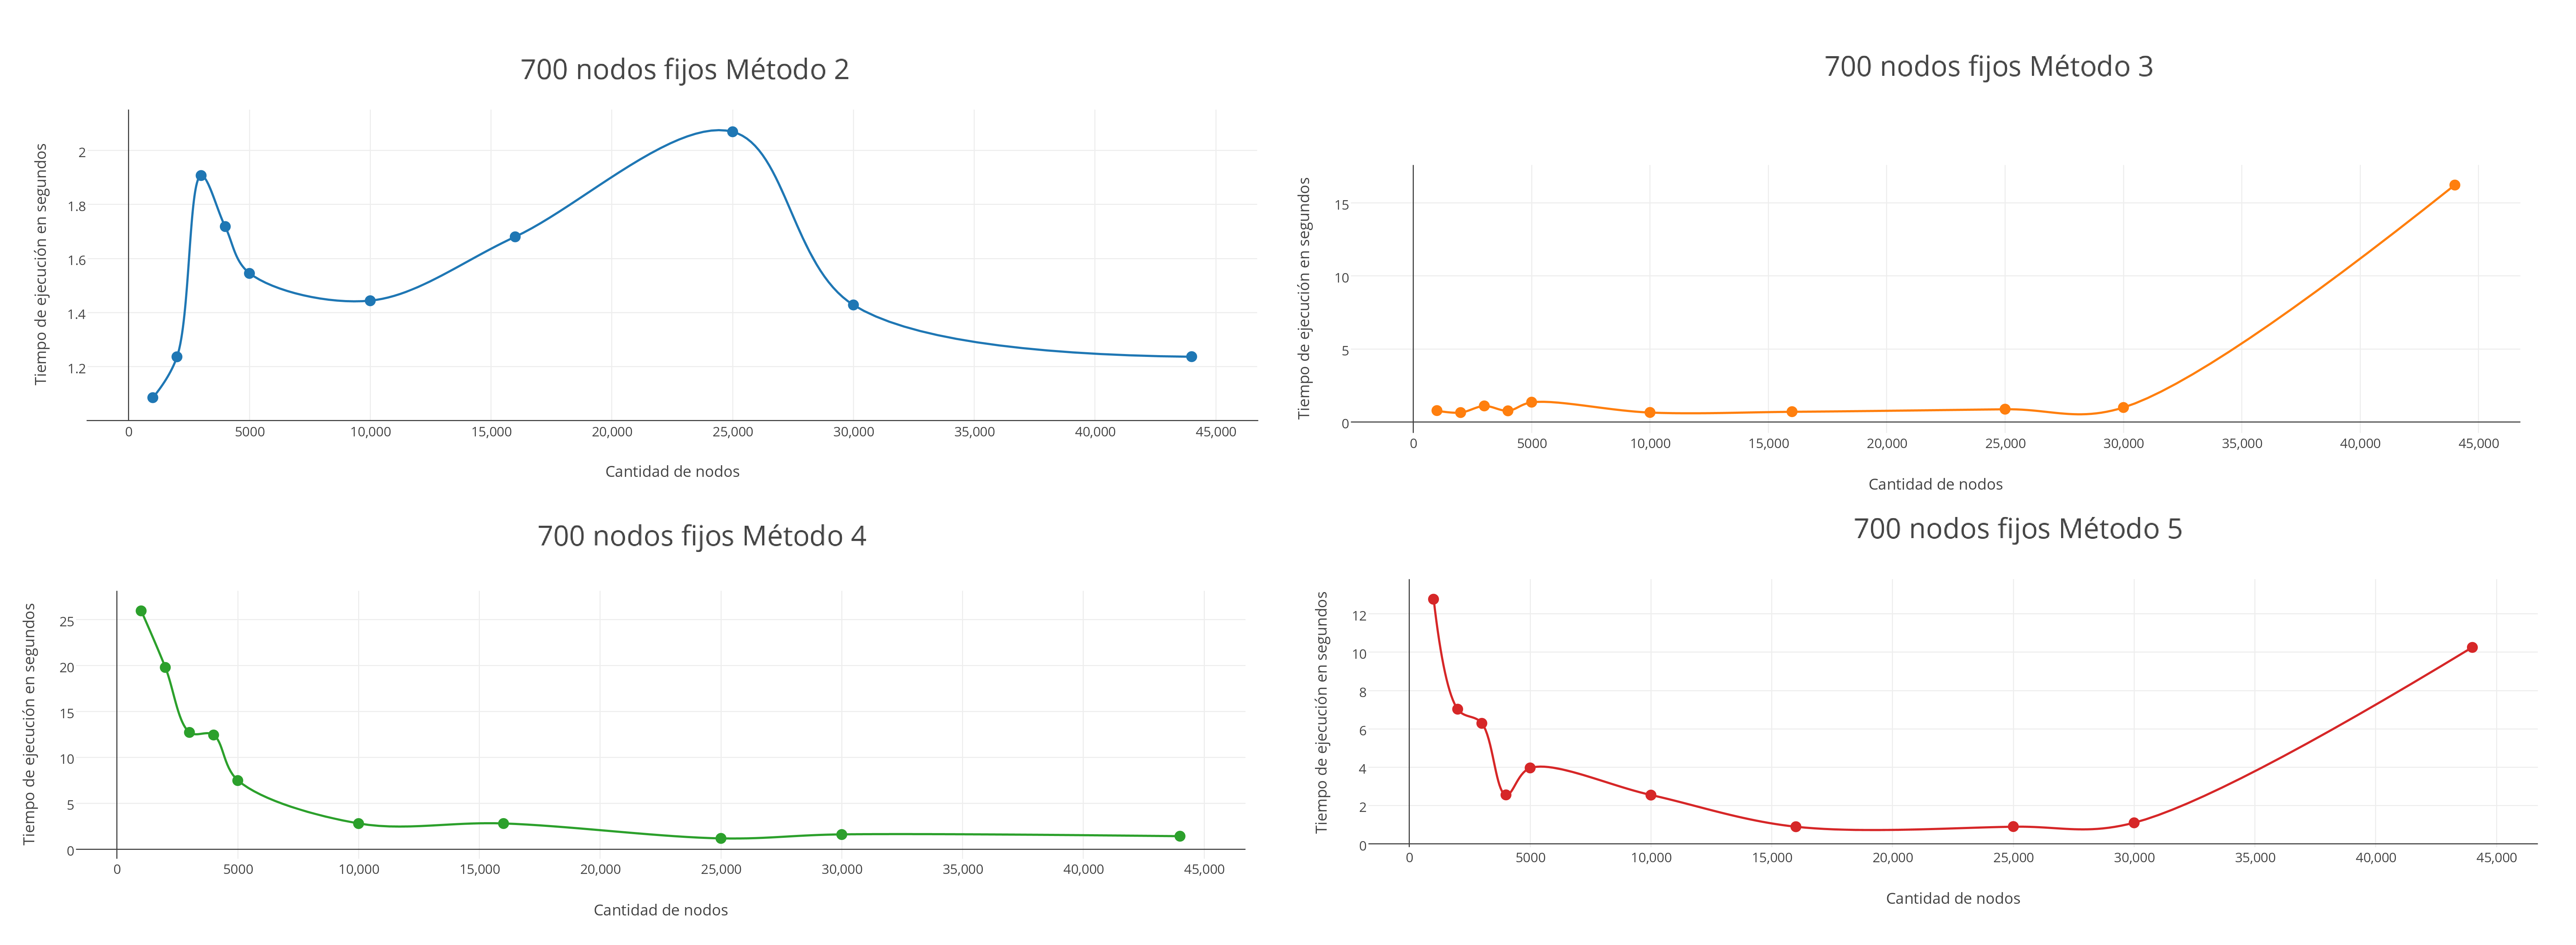
\includegraphics[scale=0.08]{imagenes/local/tiempos/700nodos2.png}
% 	\caption{}
%	\label{10Nodos}
   \end{center}
 \end{figure} 
 
Nos pareci\'o un caso notable de distinci\'on el de 700 nodos fijos, cuando se analizan los m\'etodos por separado. 

Si bien a ciencia cierta no se puede asignar a qu\'e funci\'on pertenece cada curva, pero se pueden notar las \textcolor{red}{ra\'ices (?} que poseen las curvas. De modo que se aprecia un comportamiento no estrictamente creciente. 

 \newpage
\subsubsection{Contrastaci\'on emp\'irica de la complejidad}

Se quiso linealizar los tiempos de ejecuci\'on con el fin de poder contrastar de manera \'optima las complejidades emp\'iricas con las te\'oricas. Sin embargo, esto no fue posible debido a que los tiempos de ejecuci\'on son muy peque\~nos y al dividirlos por la cantidad de nodos los resultados obtenidos no generan gr\'aficos de real inter\'es.\\

A continuaci\'on se exponen los tiempos de ejecuci\'on para los distintos m\'etodos, considerando grafos Ciclo y grafos Completos:

  \begin{figure}[h!]
   \begin{center}
 	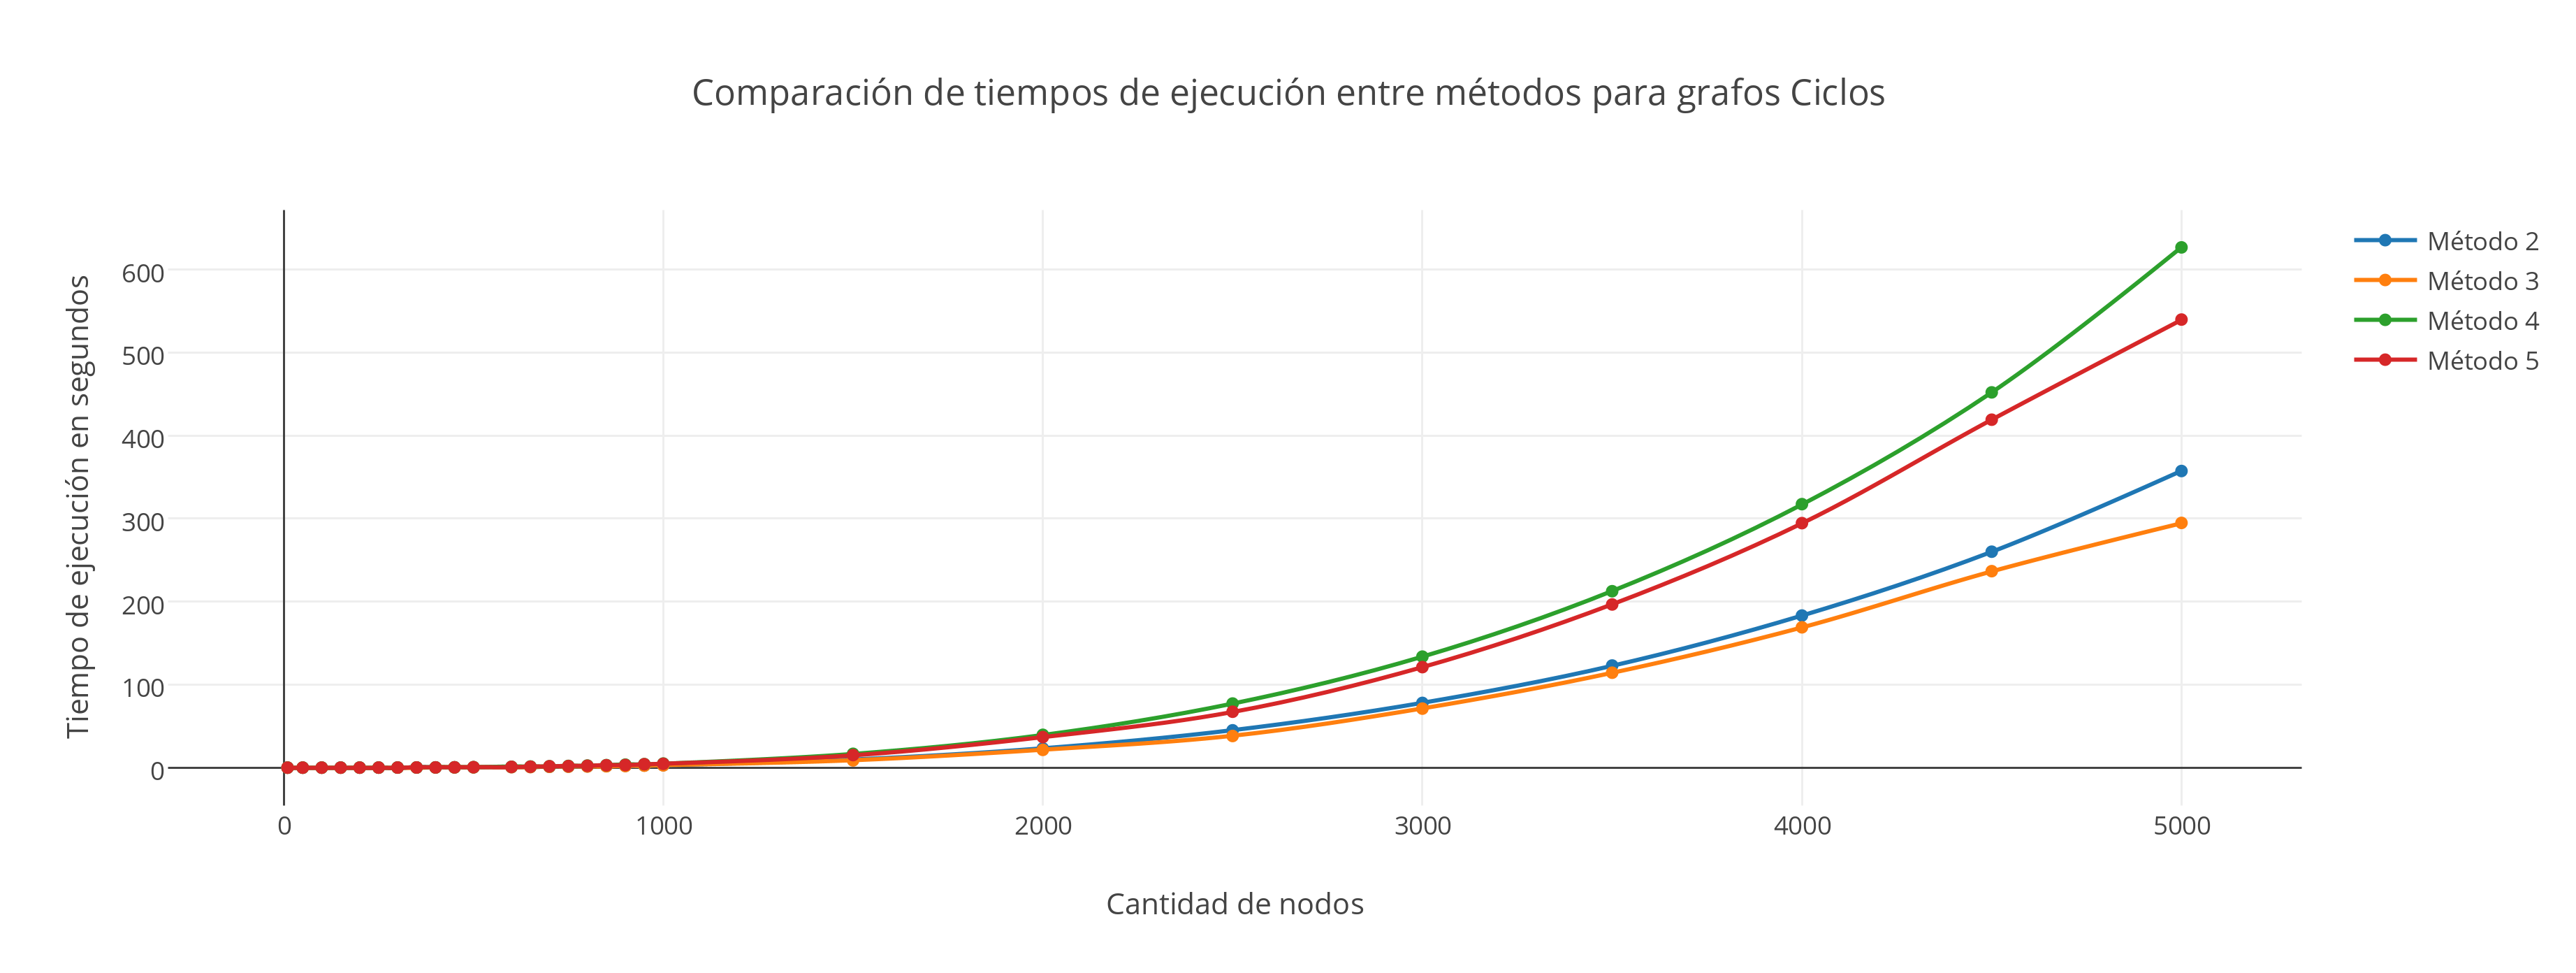
\includegraphics[scale=0.55]{imagenes/local/tiempos/ciclos.png}
% 	\caption{}
%	\label{10Nodos}
   \end{center}
 \end{figure} 
 
Los tiempos de ejecuci\'on para grafos Ciclos se condicen con los gr\'aficos de la secci\'on \ref{tiempos}. Esto significa que los \textbf{m\'etodos 4} y \textbf{5} poseen mayor tiempo de ejecuci\'on y finalmente, el \textbf{m\'etodo 2} preserva el menor.

Todas las curvas presentan un comportamiento que se asemeja a un valor cuadr\'atico  o c\'ubico, ya que si bien la complejidad te\'orica es de \textcolor{red}{$O(n^5)$ (?)} al tener s\'olo dos vecinos cada nodo las listas de adyacencia se recorren en $O(2)\subseteq O(1)$.
 
   \begin{figure}[h!]
   \begin{center}
 	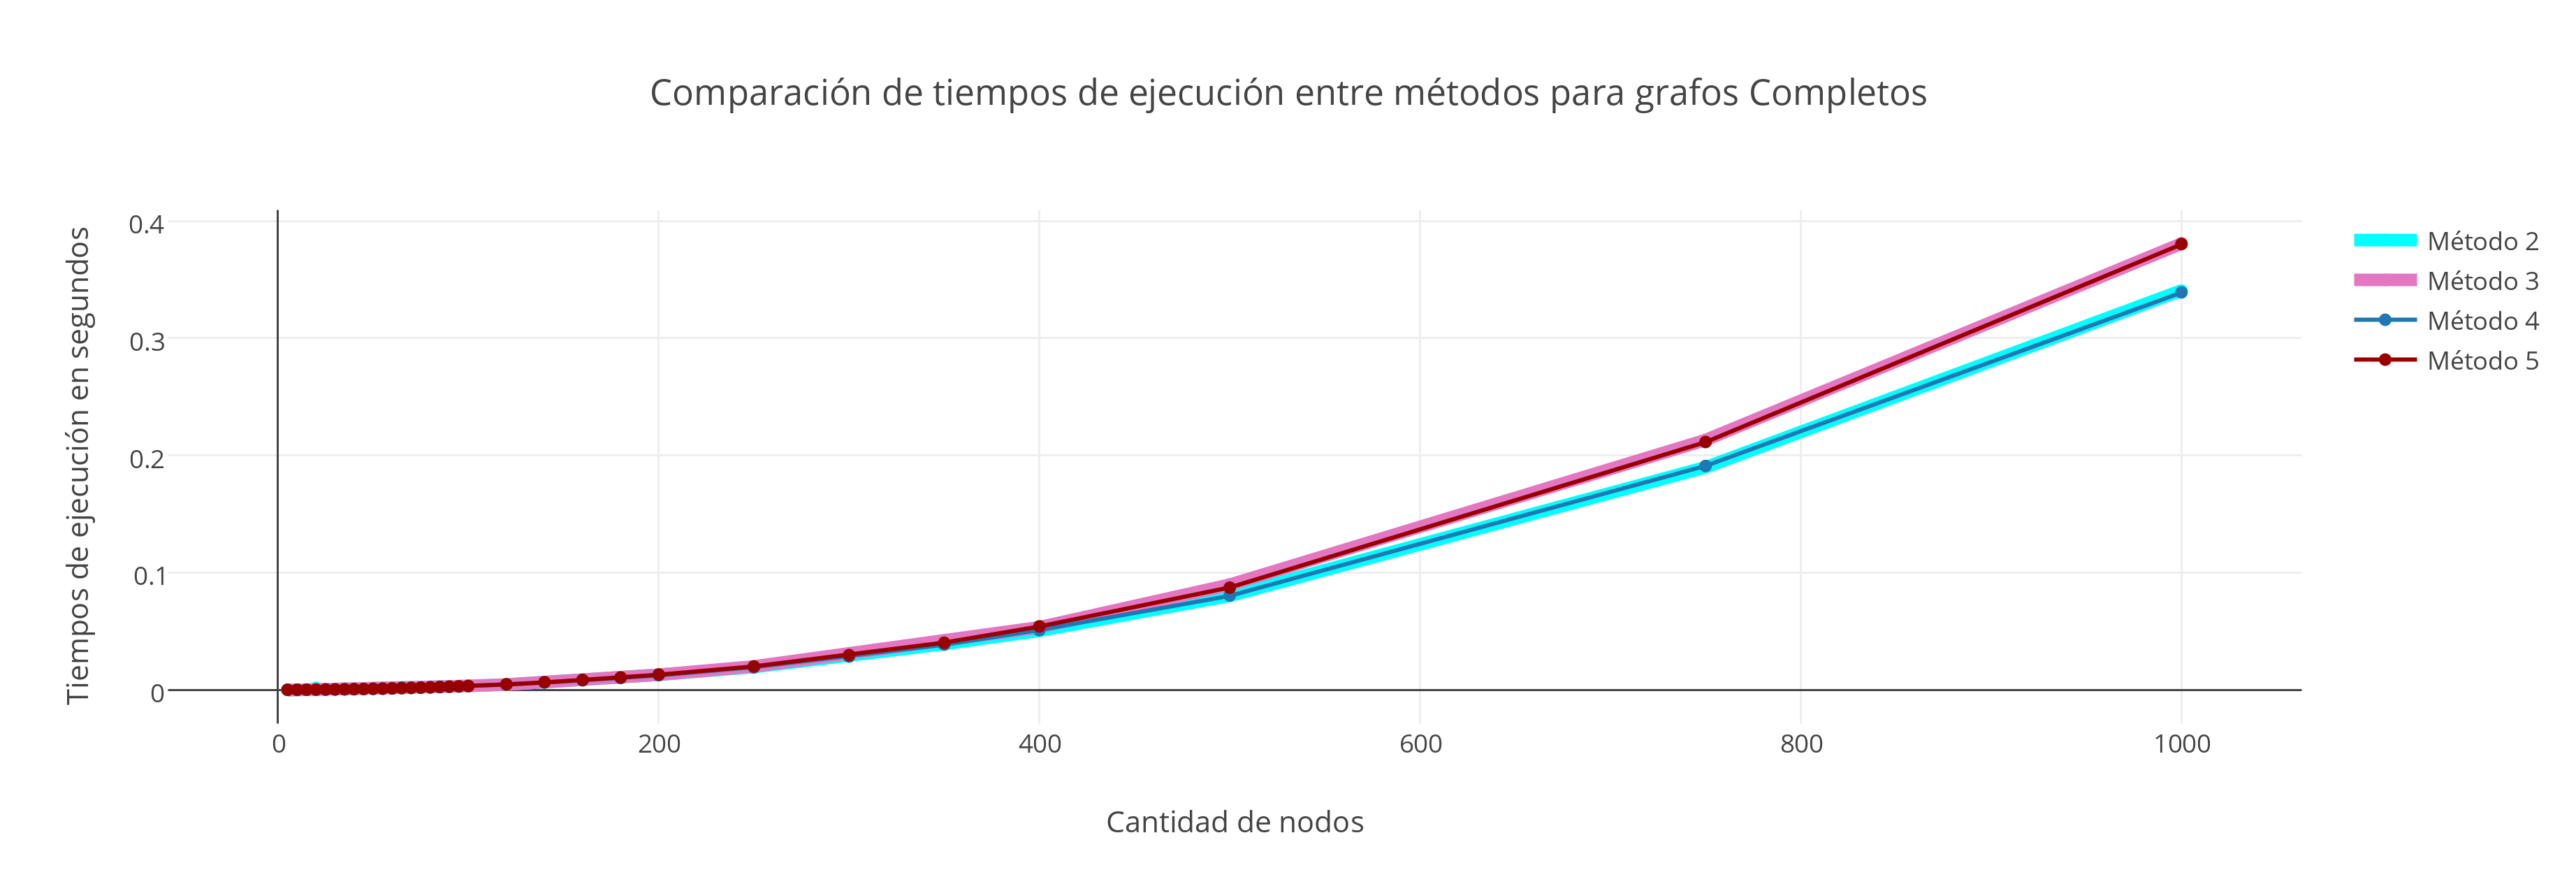
\includegraphics[scale=0.55]{imagenes/local/tiempos/completos.png}
% 	\caption{}
%	\label{10Nodos}
   \end{center}
 \end{figure} 
 
\textcolor{red}{Los grafos completos son... } 
 
\newpage
\subsubsection{Comparaci\'on soluciones Local vs Exacto}

  \begin{figure}[h!]
   \begin{center}
 	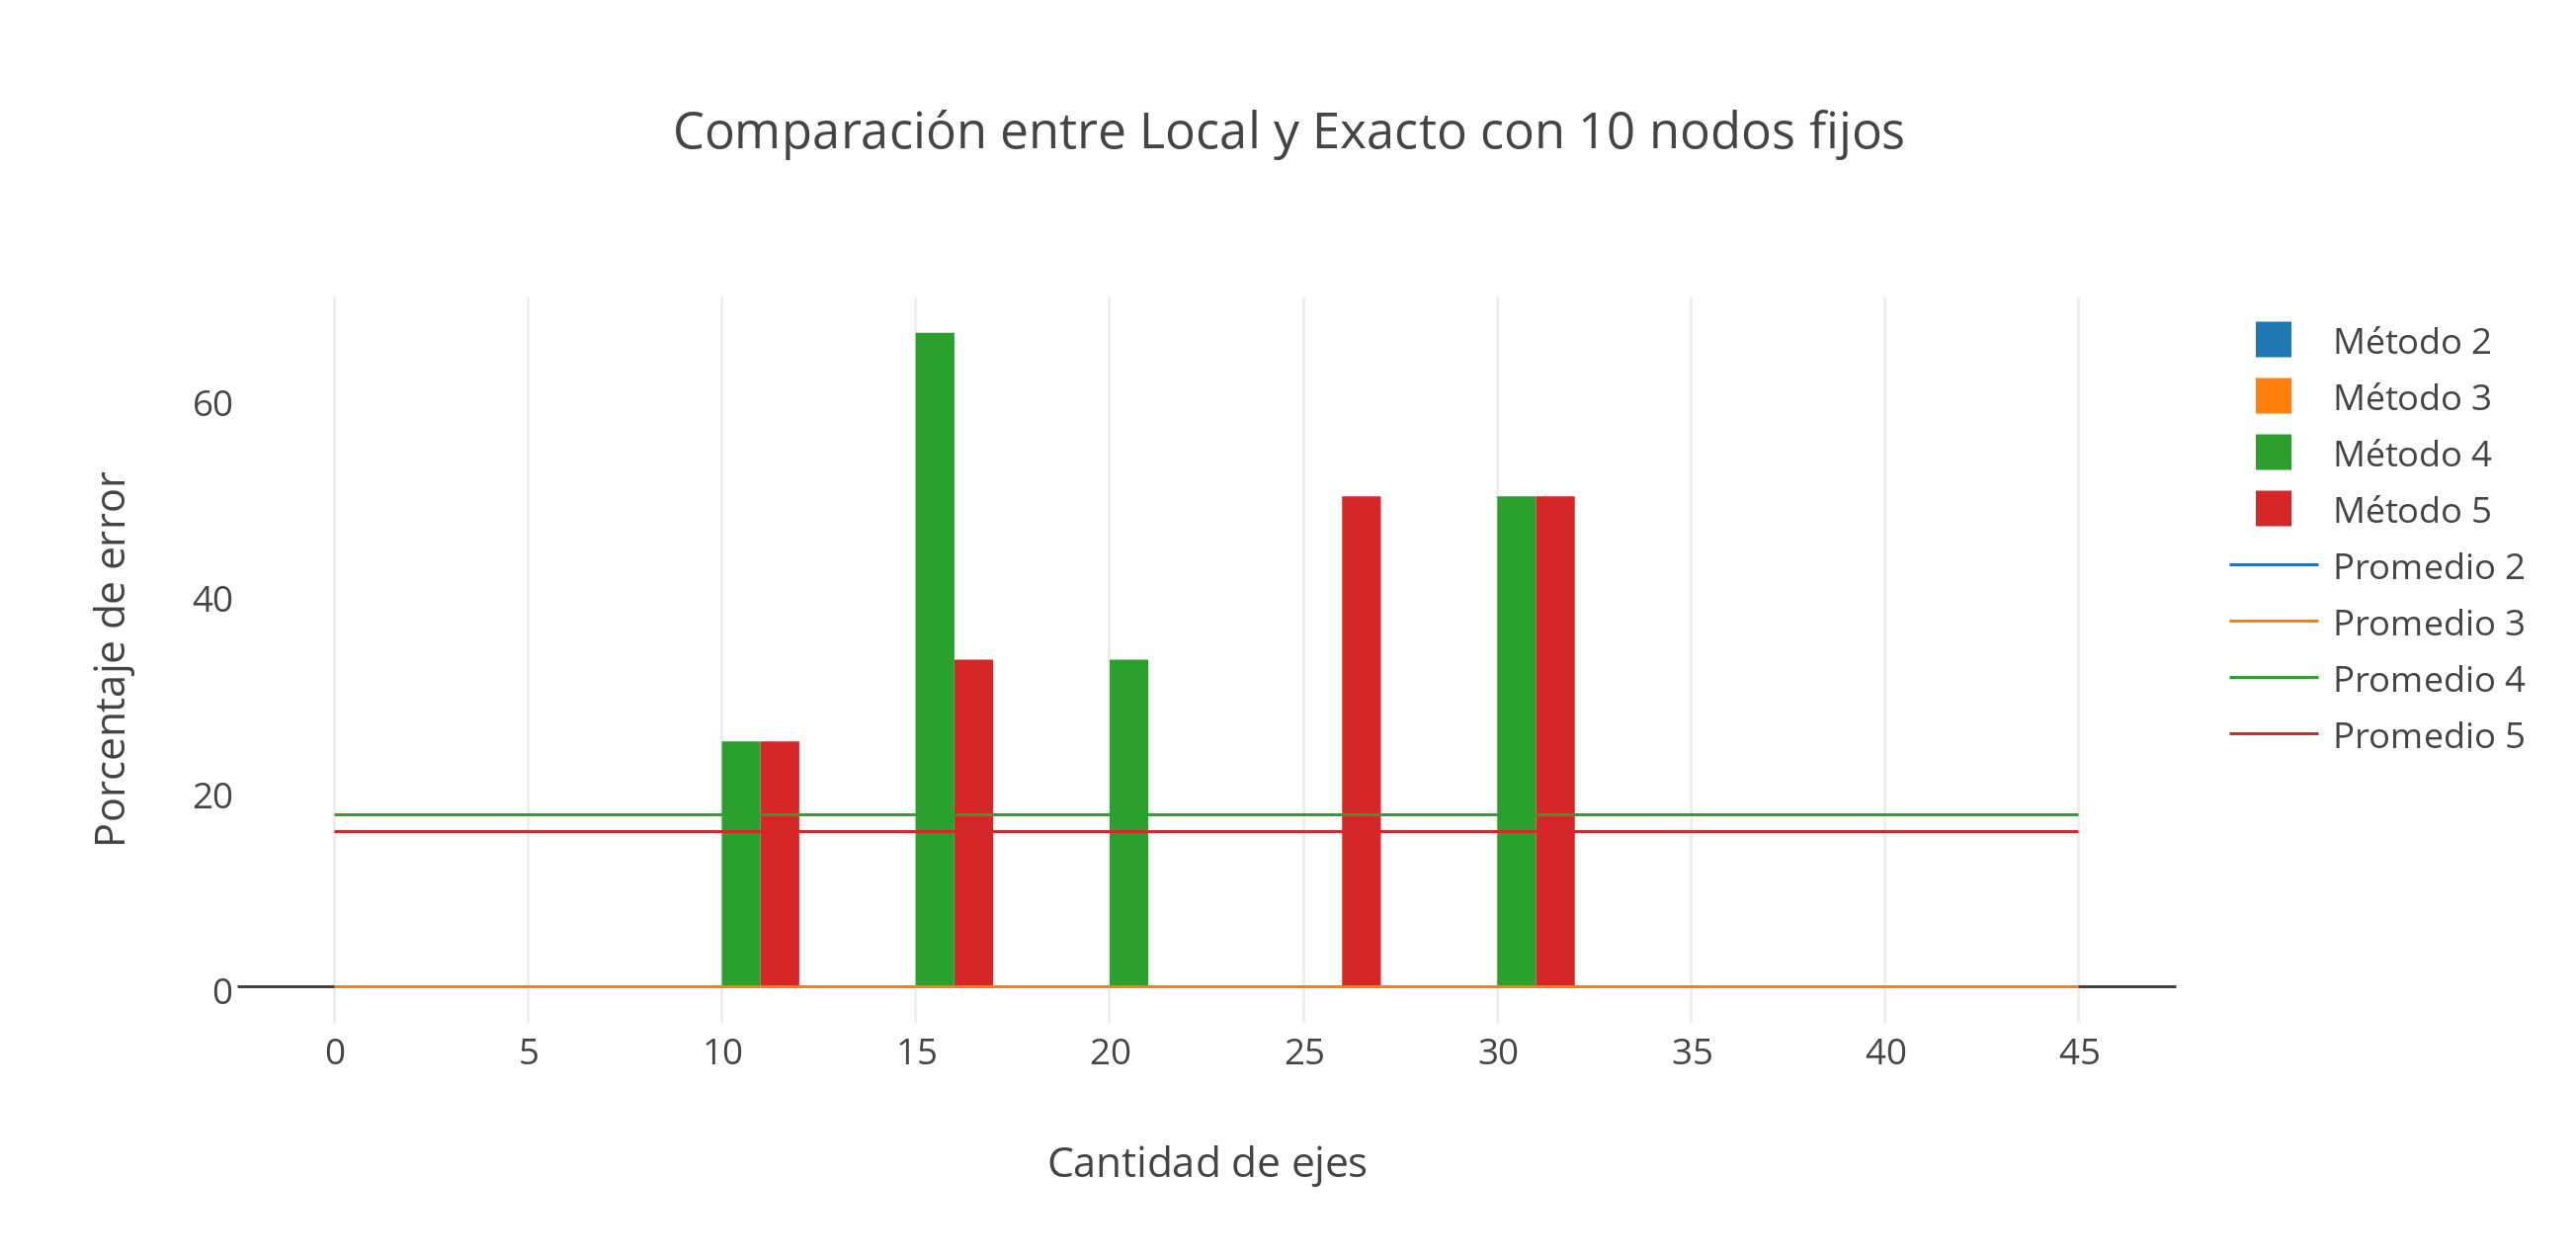
\includegraphics[scale=0.75]{imagenes/local/exacto/10nodos.png}
% 	\caption{}
%	\label{10Nodos}
   \end{center}
 \end{figure}

  \begin{figure}[h!]
   \begin{center}
 	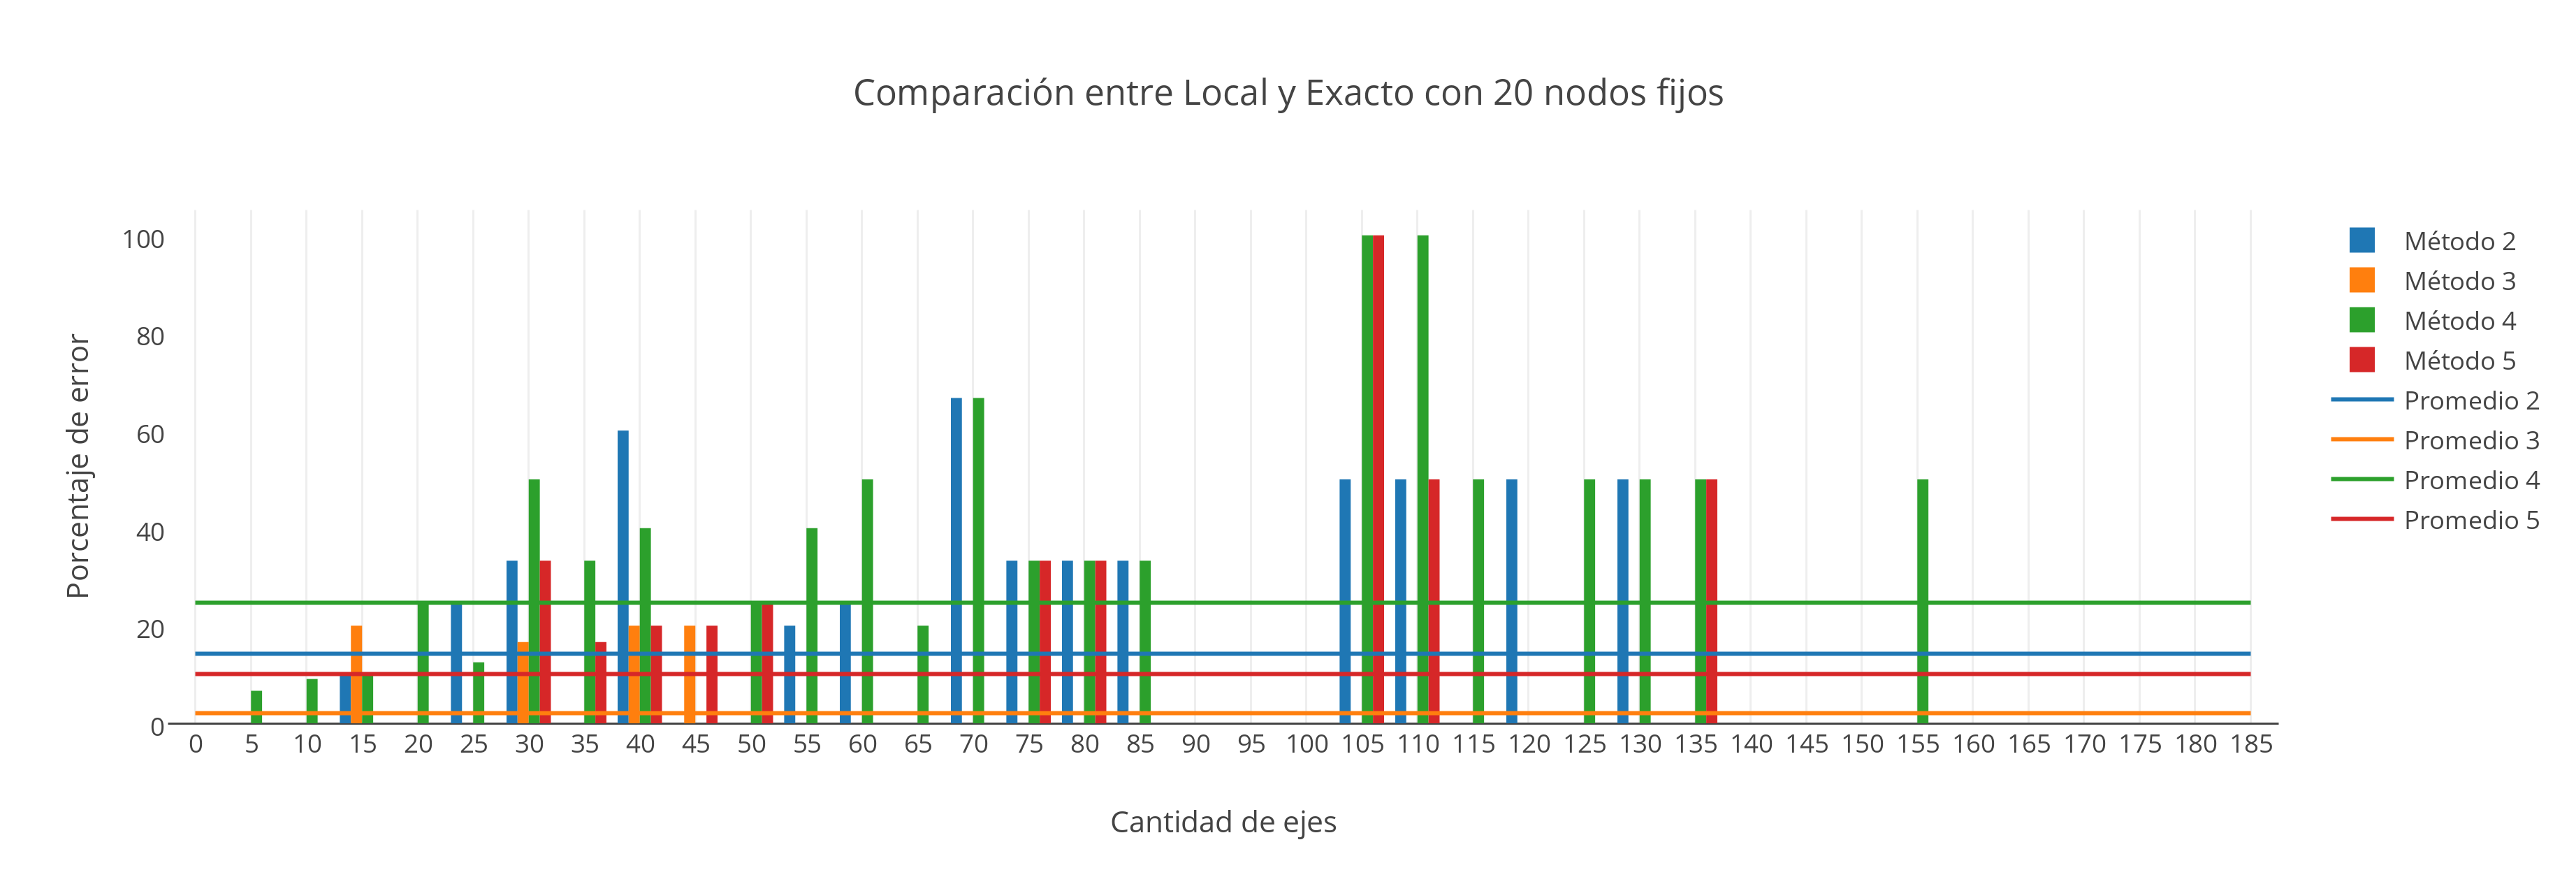
\includegraphics[scale=0.55]{imagenes/local/exacto/20nodos.png}
% 	\caption{}
%	\label{10Nodos}
   \end{center}
 \end{figure}
 
   \begin{figure}[h!]
   \begin{center}
 	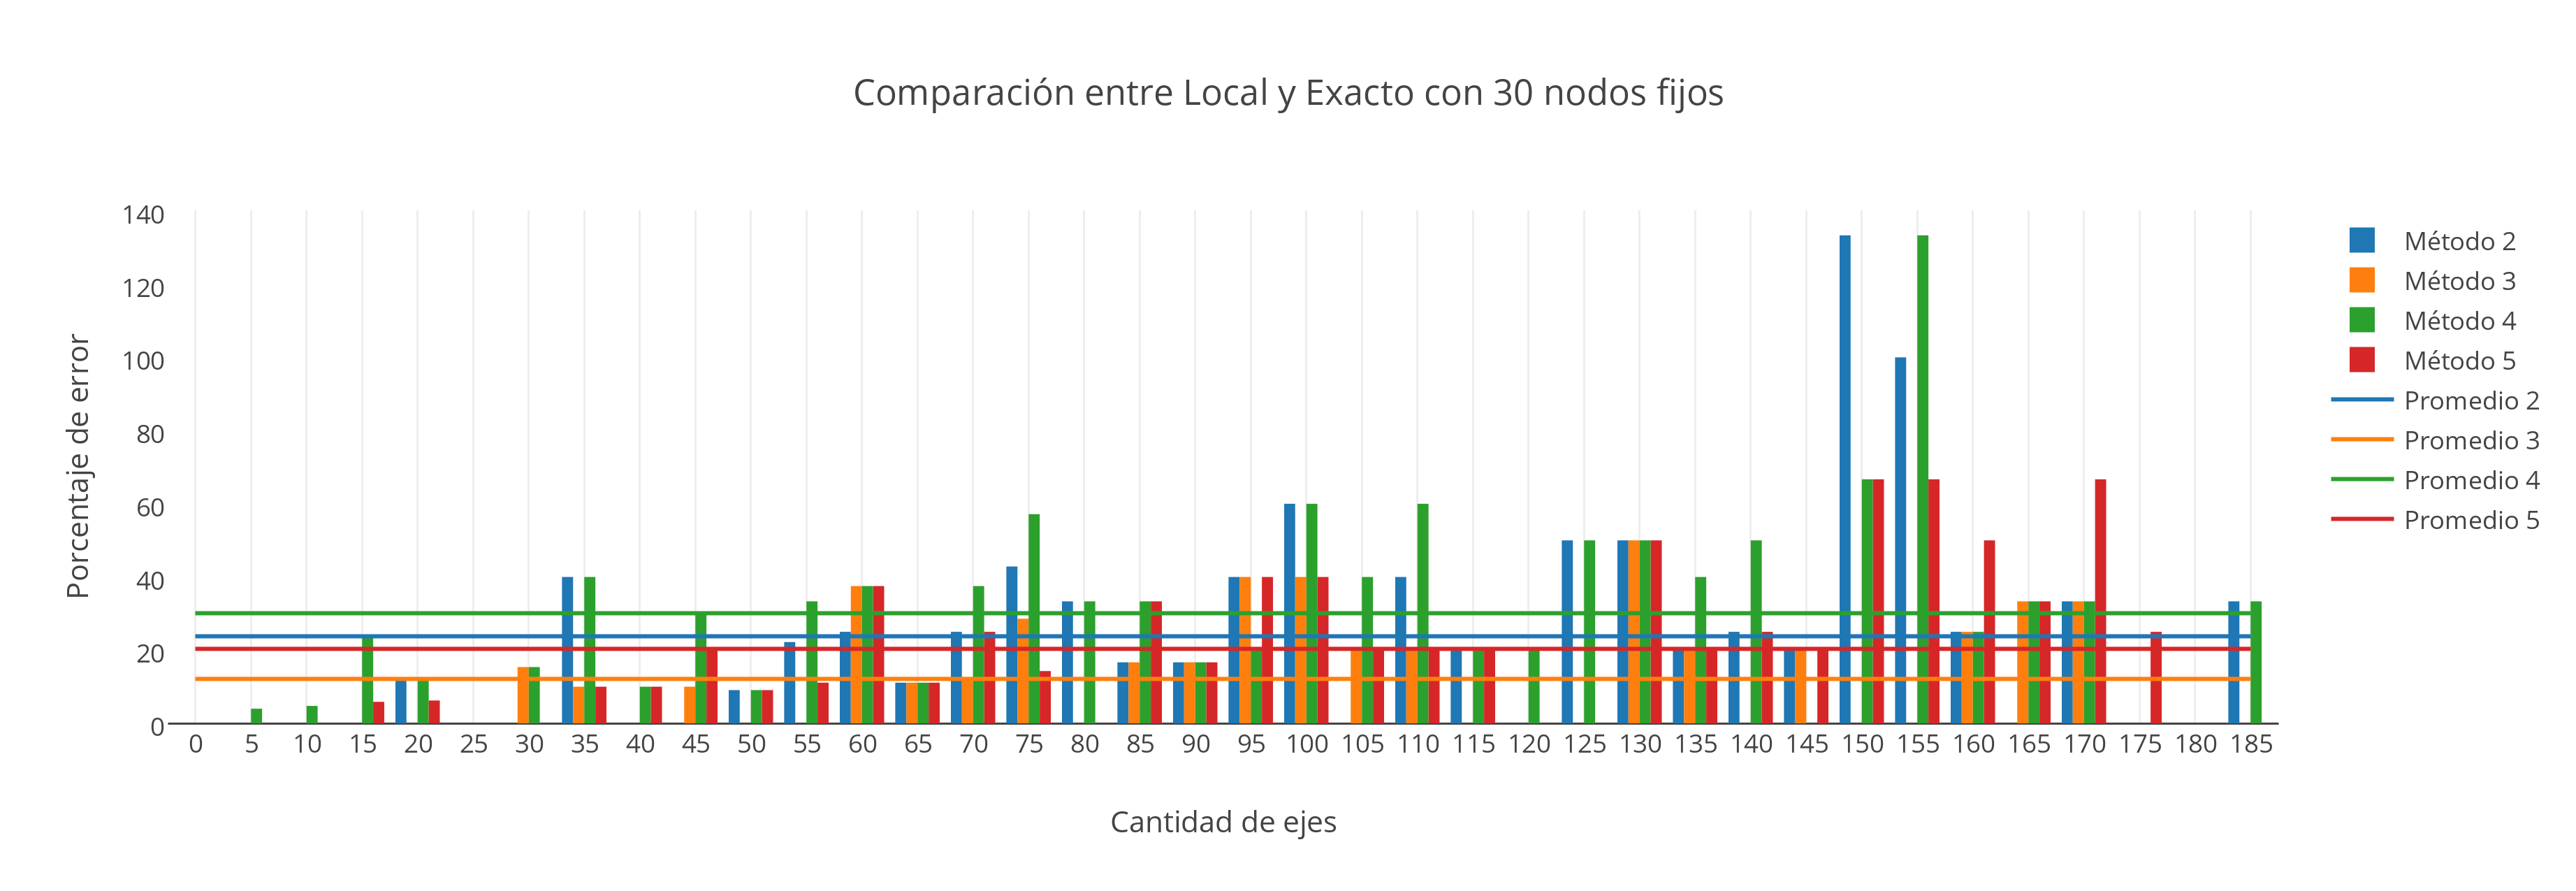
\includegraphics[scale=0.55]{imagenes/local/exacto/30nodos.png}
% 	\caption{}
%	\label{10Nodos}
   \end{center}
 \end{figure}

\newpage

  \begin{figure}[h!]
   \begin{center}
 	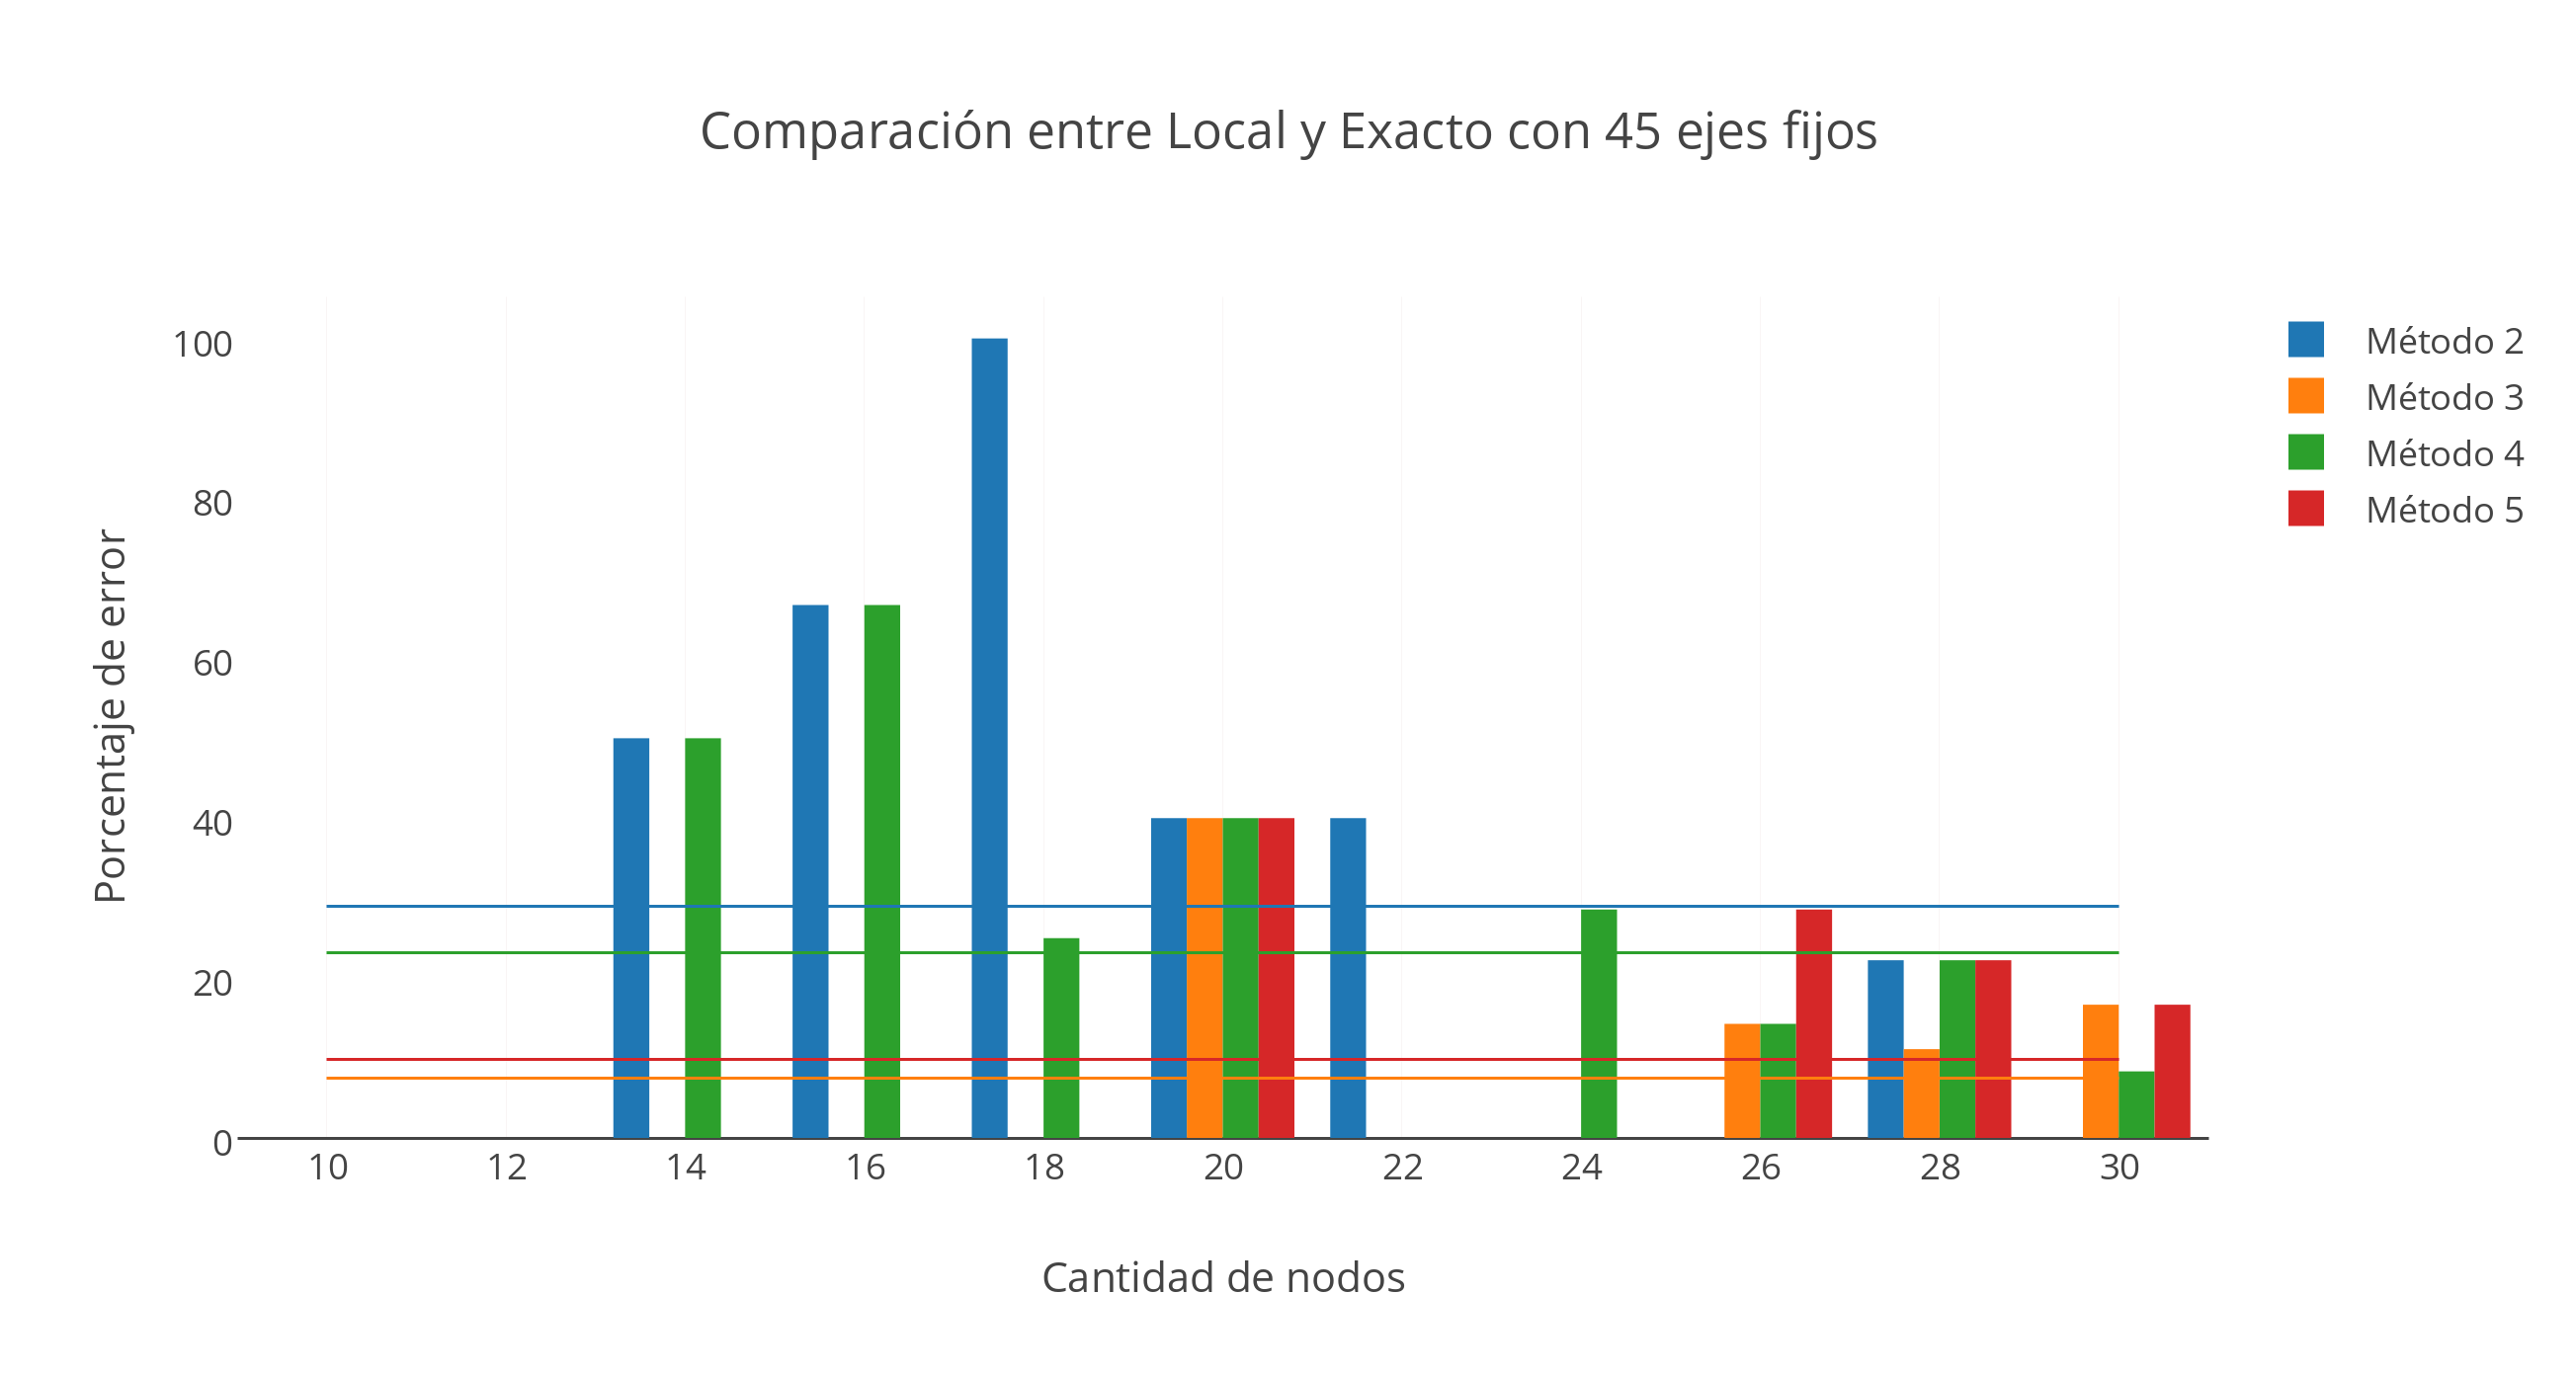
\includegraphics[scale=0.7]{imagenes/local/exacto/45ejes.png}
% 	\caption{}
%	\label{10Nodos}
   \end{center}
 \end{figure} 
 
  \begin{figure}[h!]
   \begin{center}
 	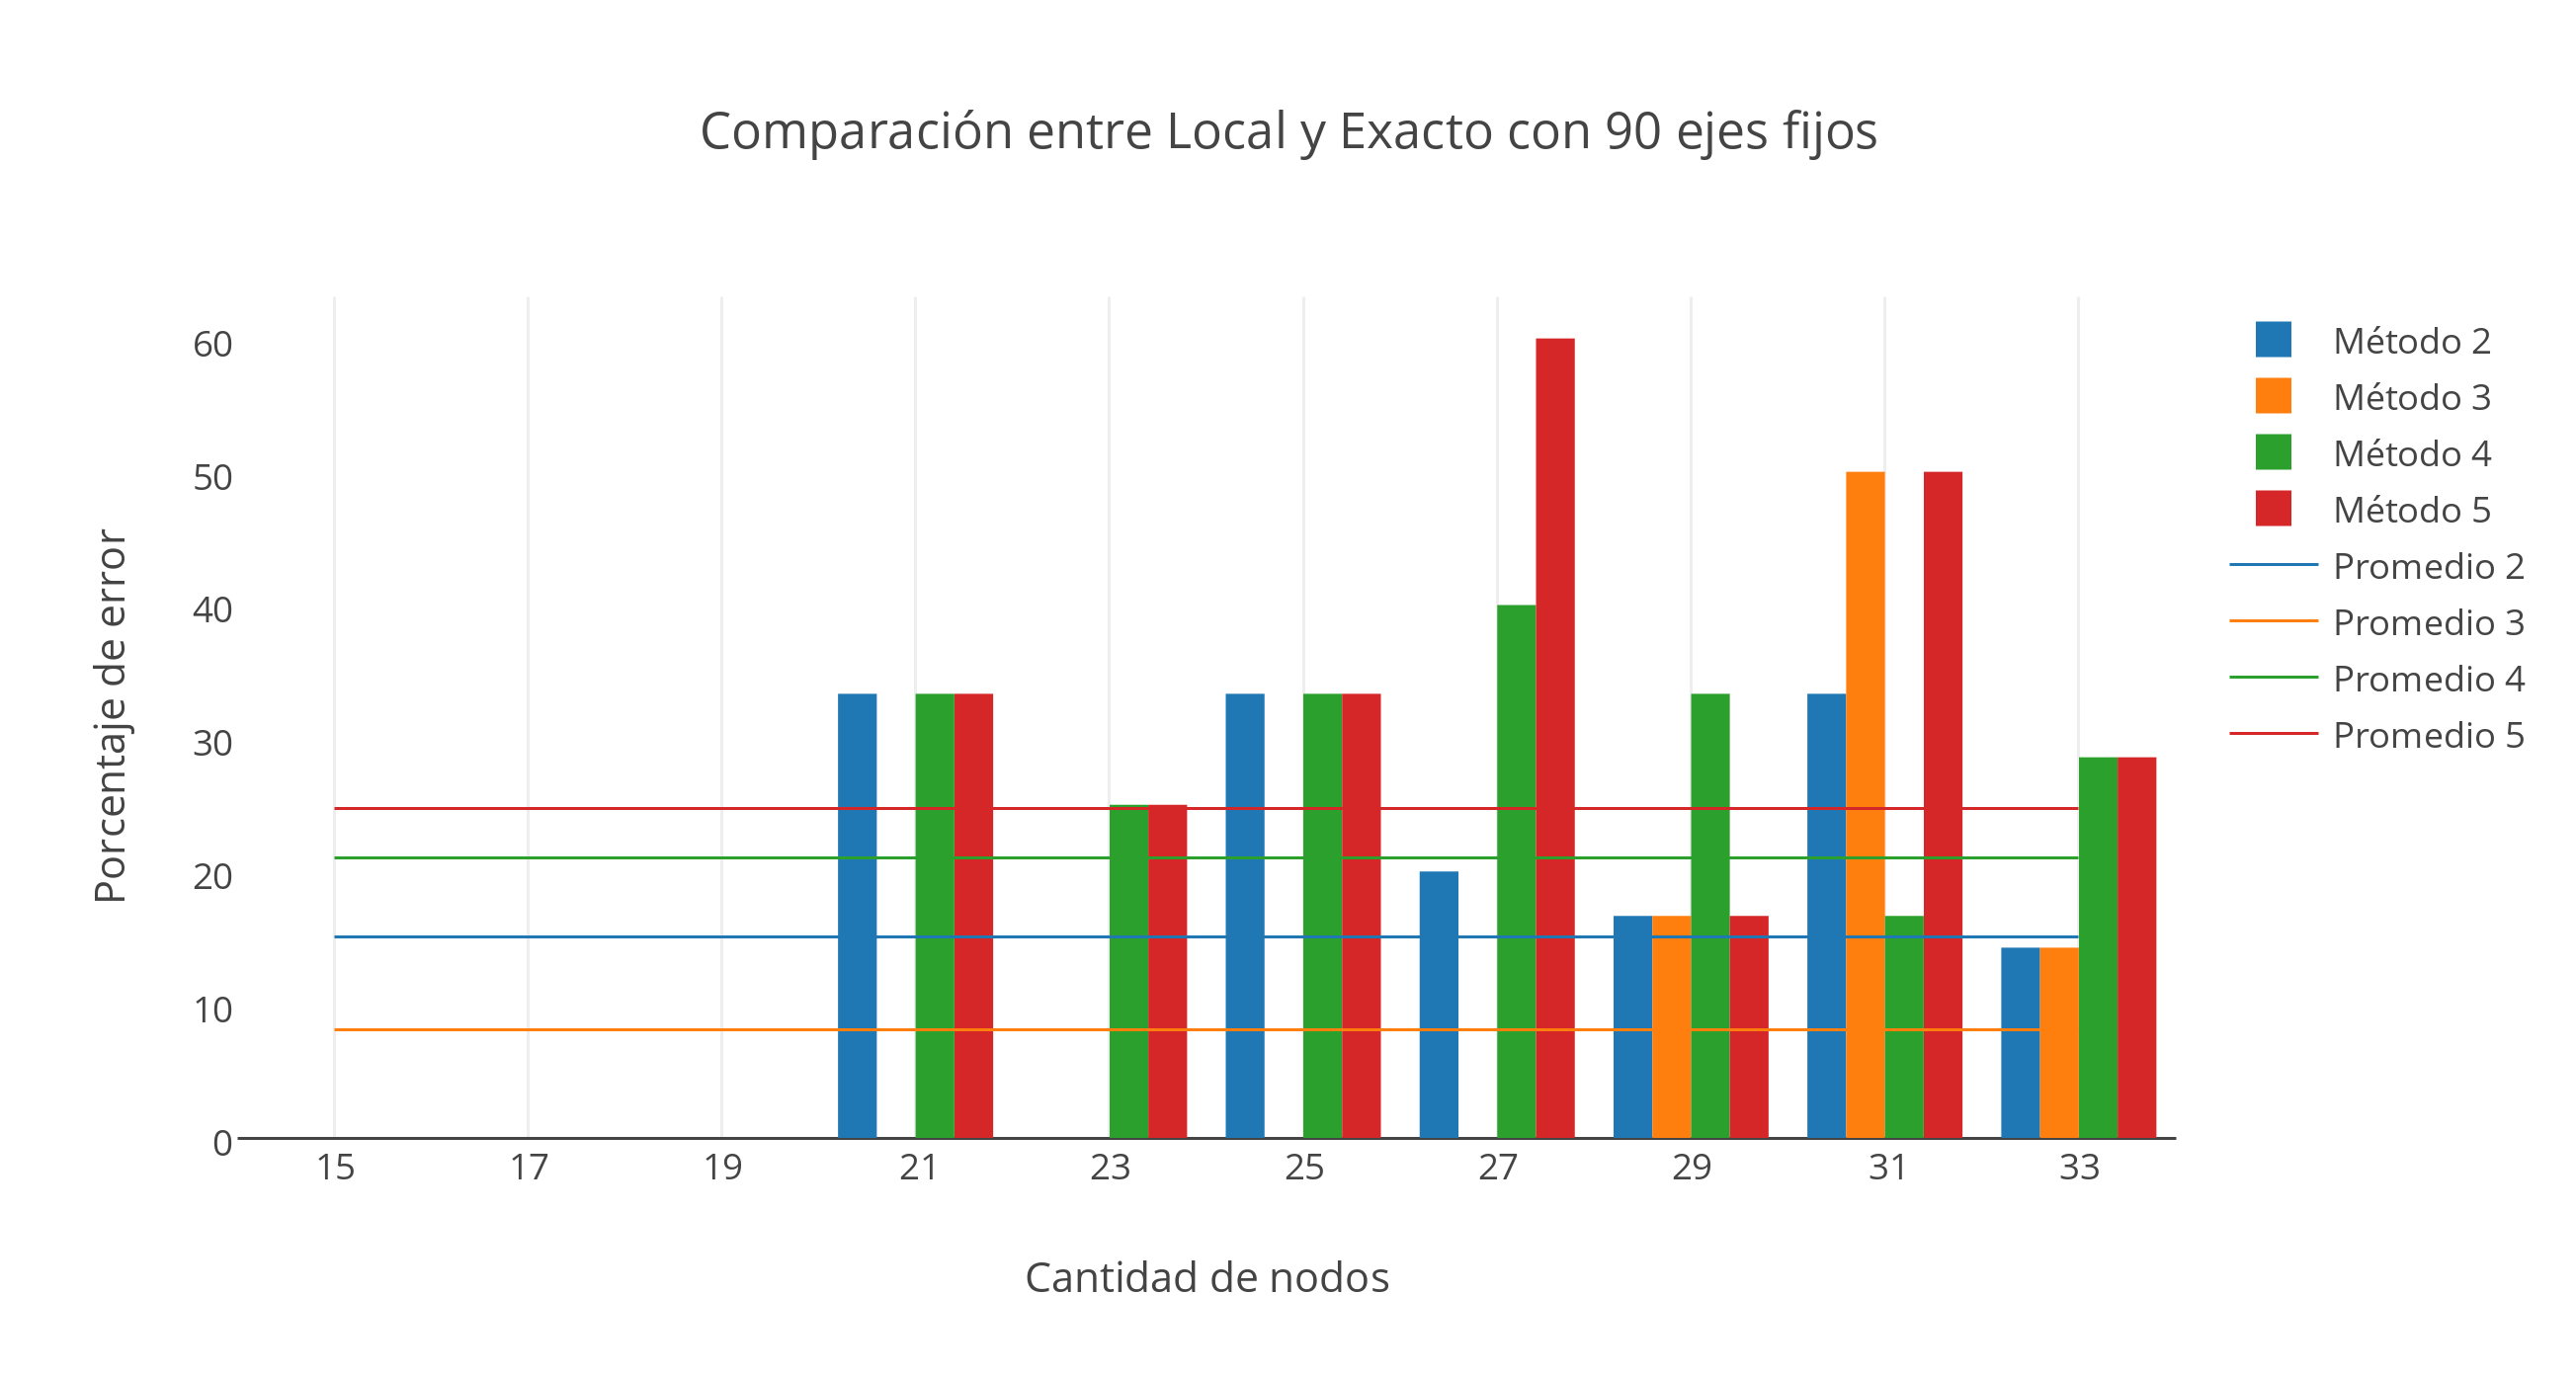
\includegraphics[scale=0.7]{imagenes/local/exacto/90ejes.png}
% 	\caption{}
%	\label{10Nodos}
   \end{center}
 \end{figure} 
 
 \newpage
  \begin{figure}[h!]
   \begin{center}
 	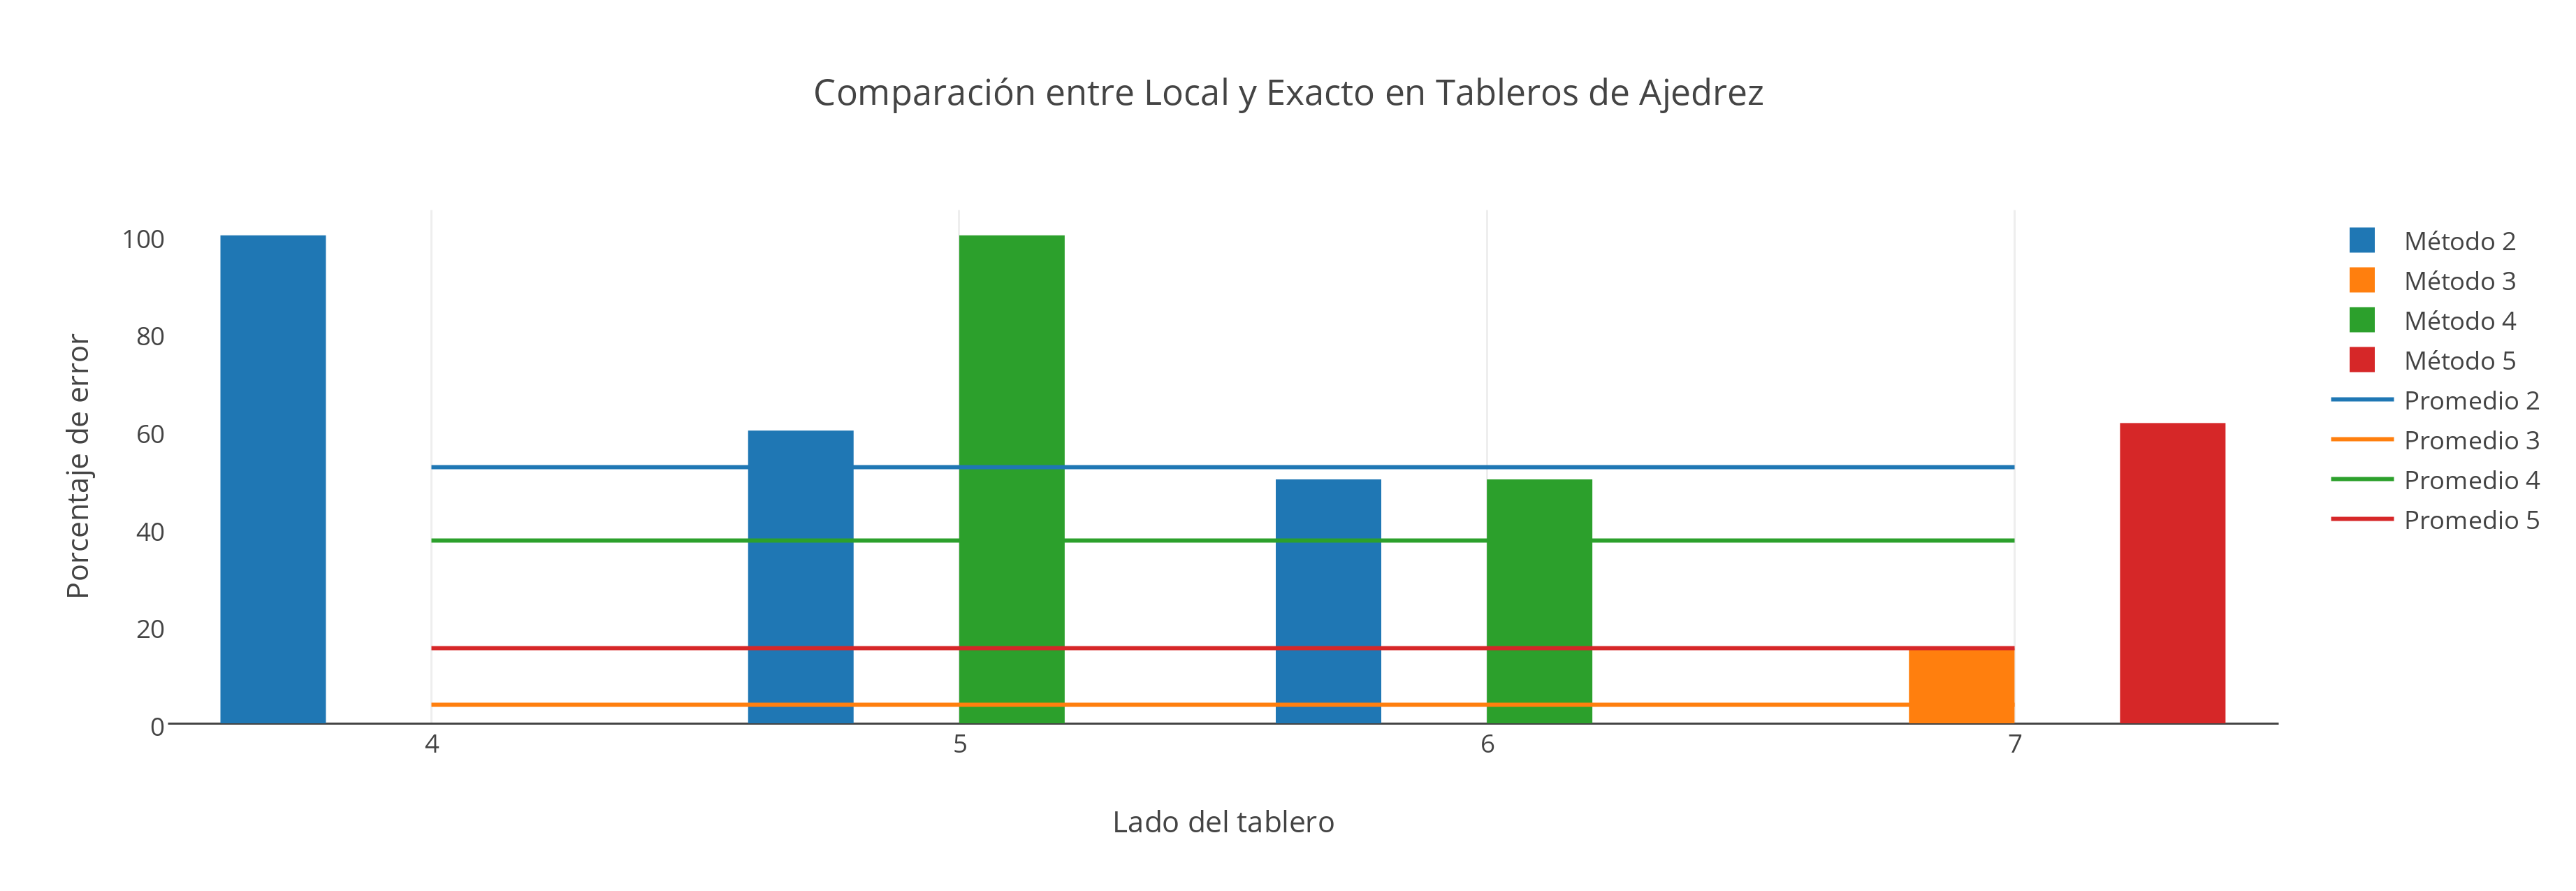
\includegraphics[scale=0.55]{imagenes/local/exacto/tableros.png}
% 	\caption{}
%	\label{10Nodos}
   \end{center}
 \end{figure} 
 
\newpage 
 
\subsubsection{Elecci\'on de versi\'on \'optima}

\subsubsection*{Ejes Fijos}


  \begin{figure}[h!]
   \begin{center}
 	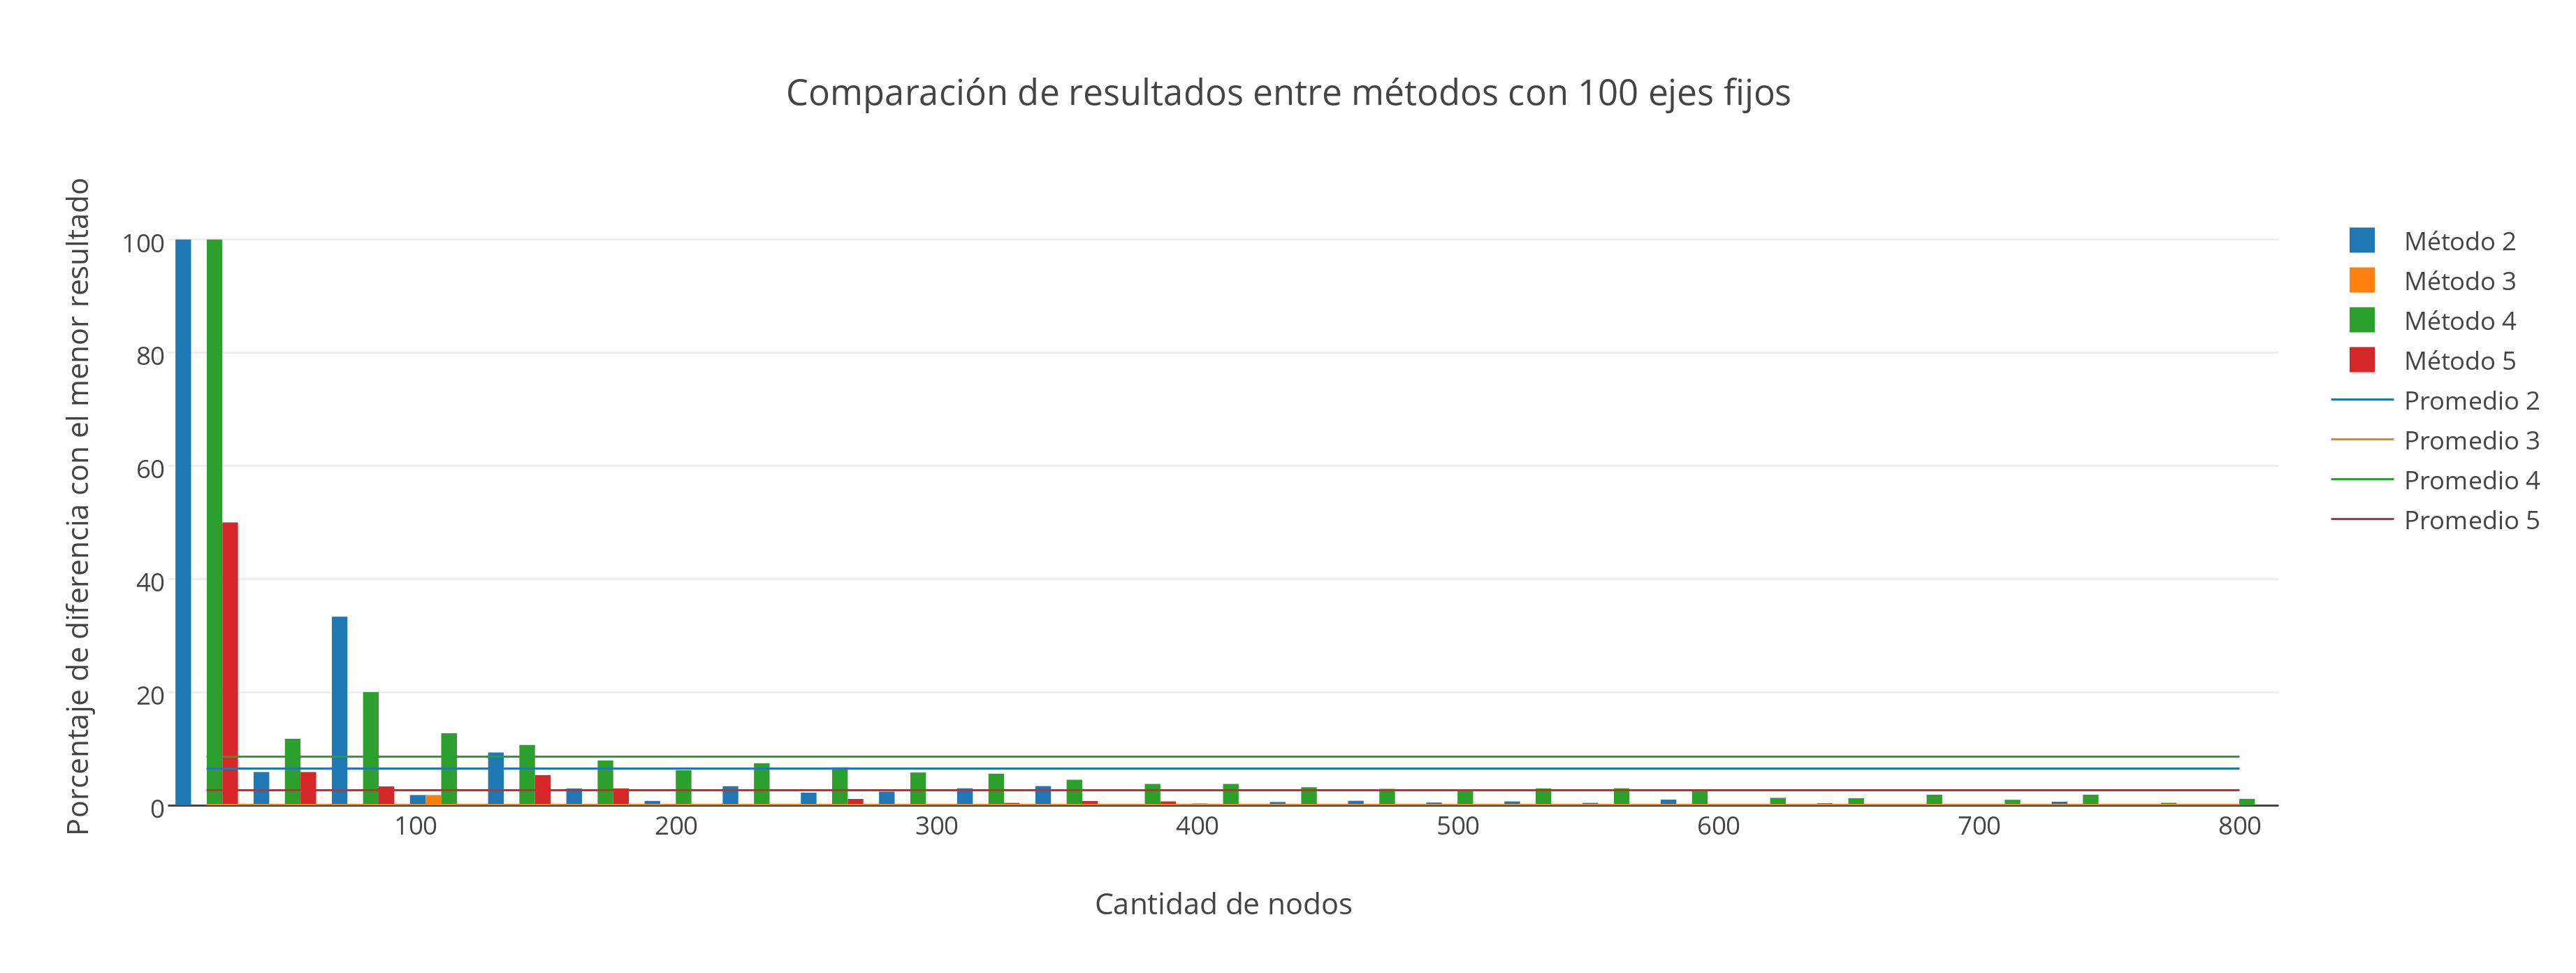
\includegraphics[scale=0.55]{imagenes/local/resultados/100ejes.png}
% 	\caption{}
%	\label{10Nodos}
   \end{center}
 \end{figure}
 

  \begin{figure}[h!]
   \begin{center}
 	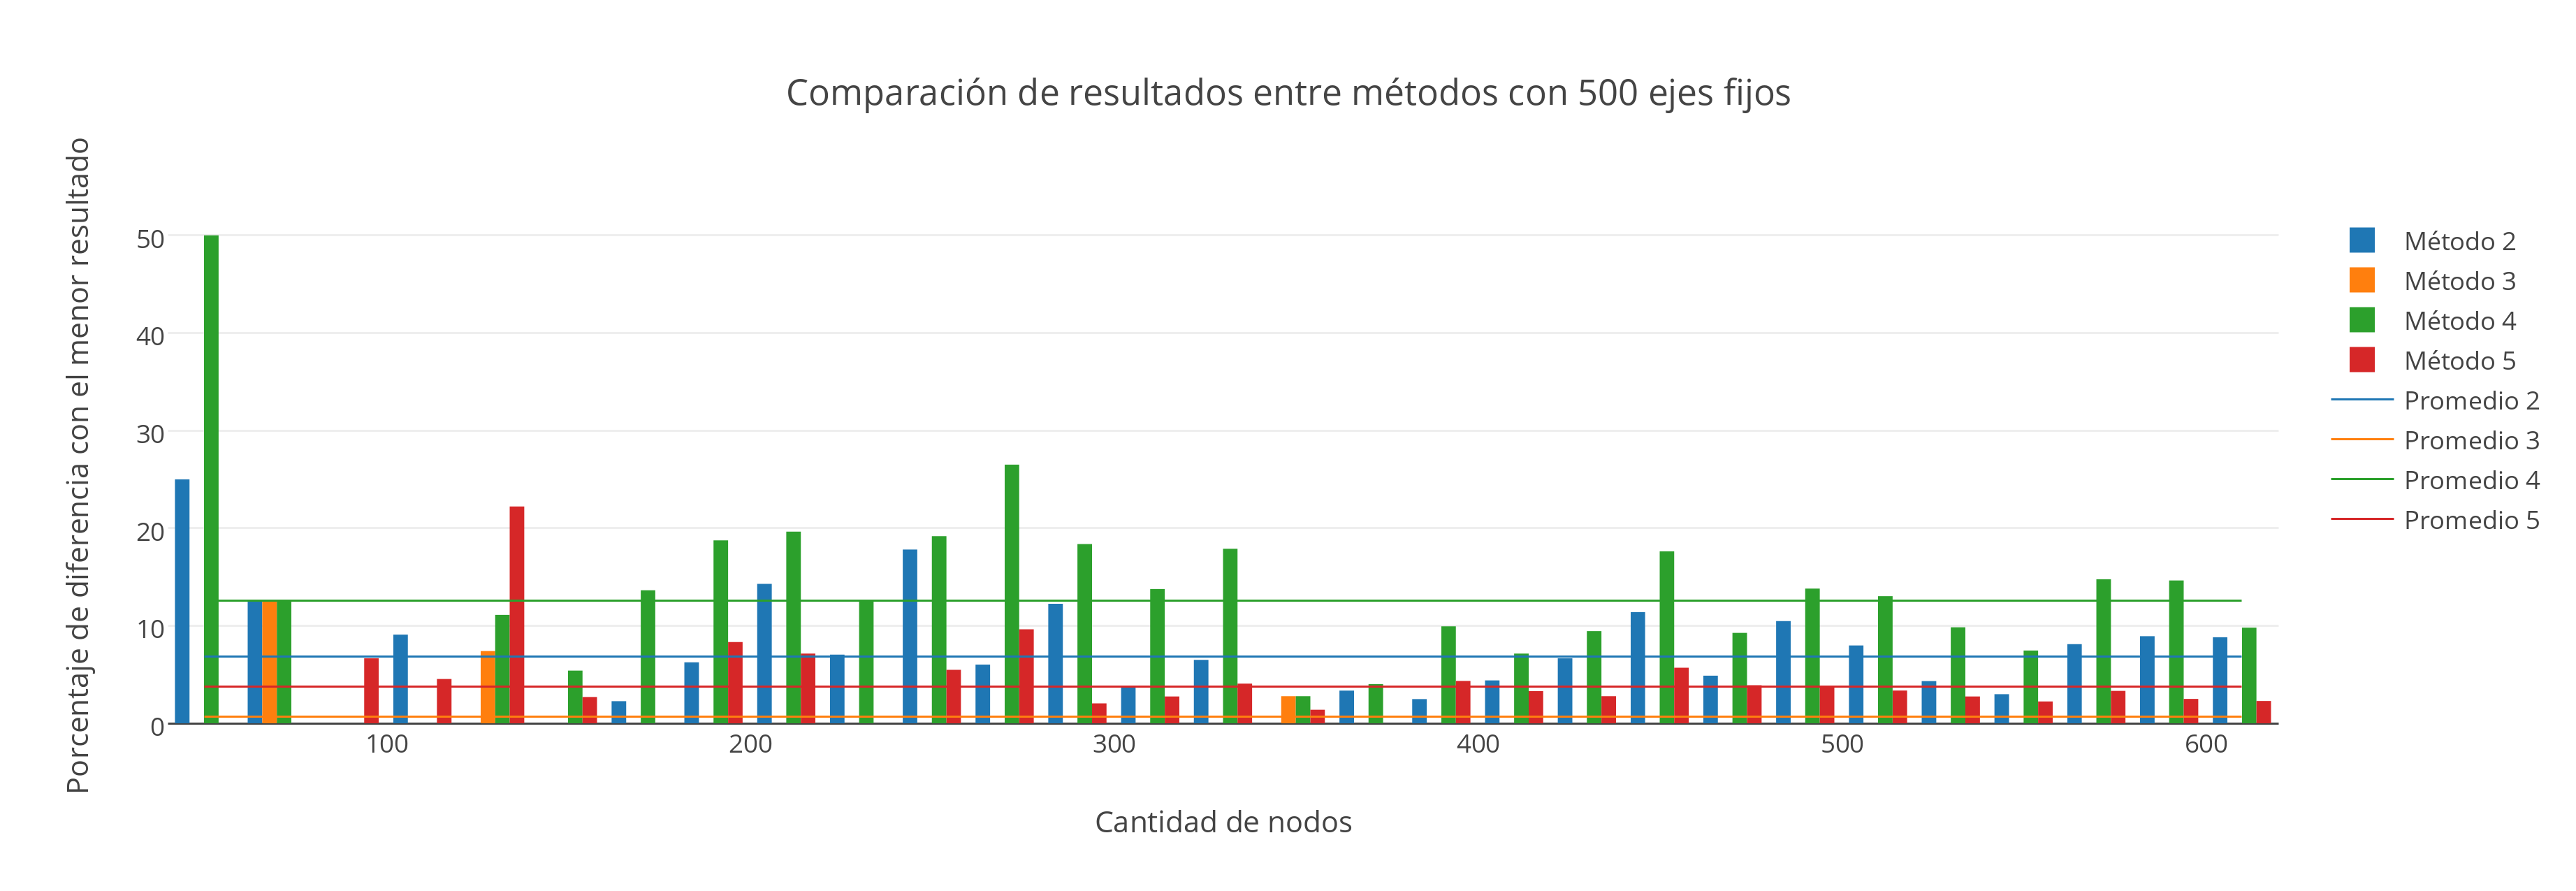
\includegraphics[scale=0.55]{imagenes/local/resultados/500ejes.png}
% 	\caption{}
%	\label{10Nodos}
   \end{center}
 \end{figure}
 
   \begin{figure}[h!]
   \begin{center}
 	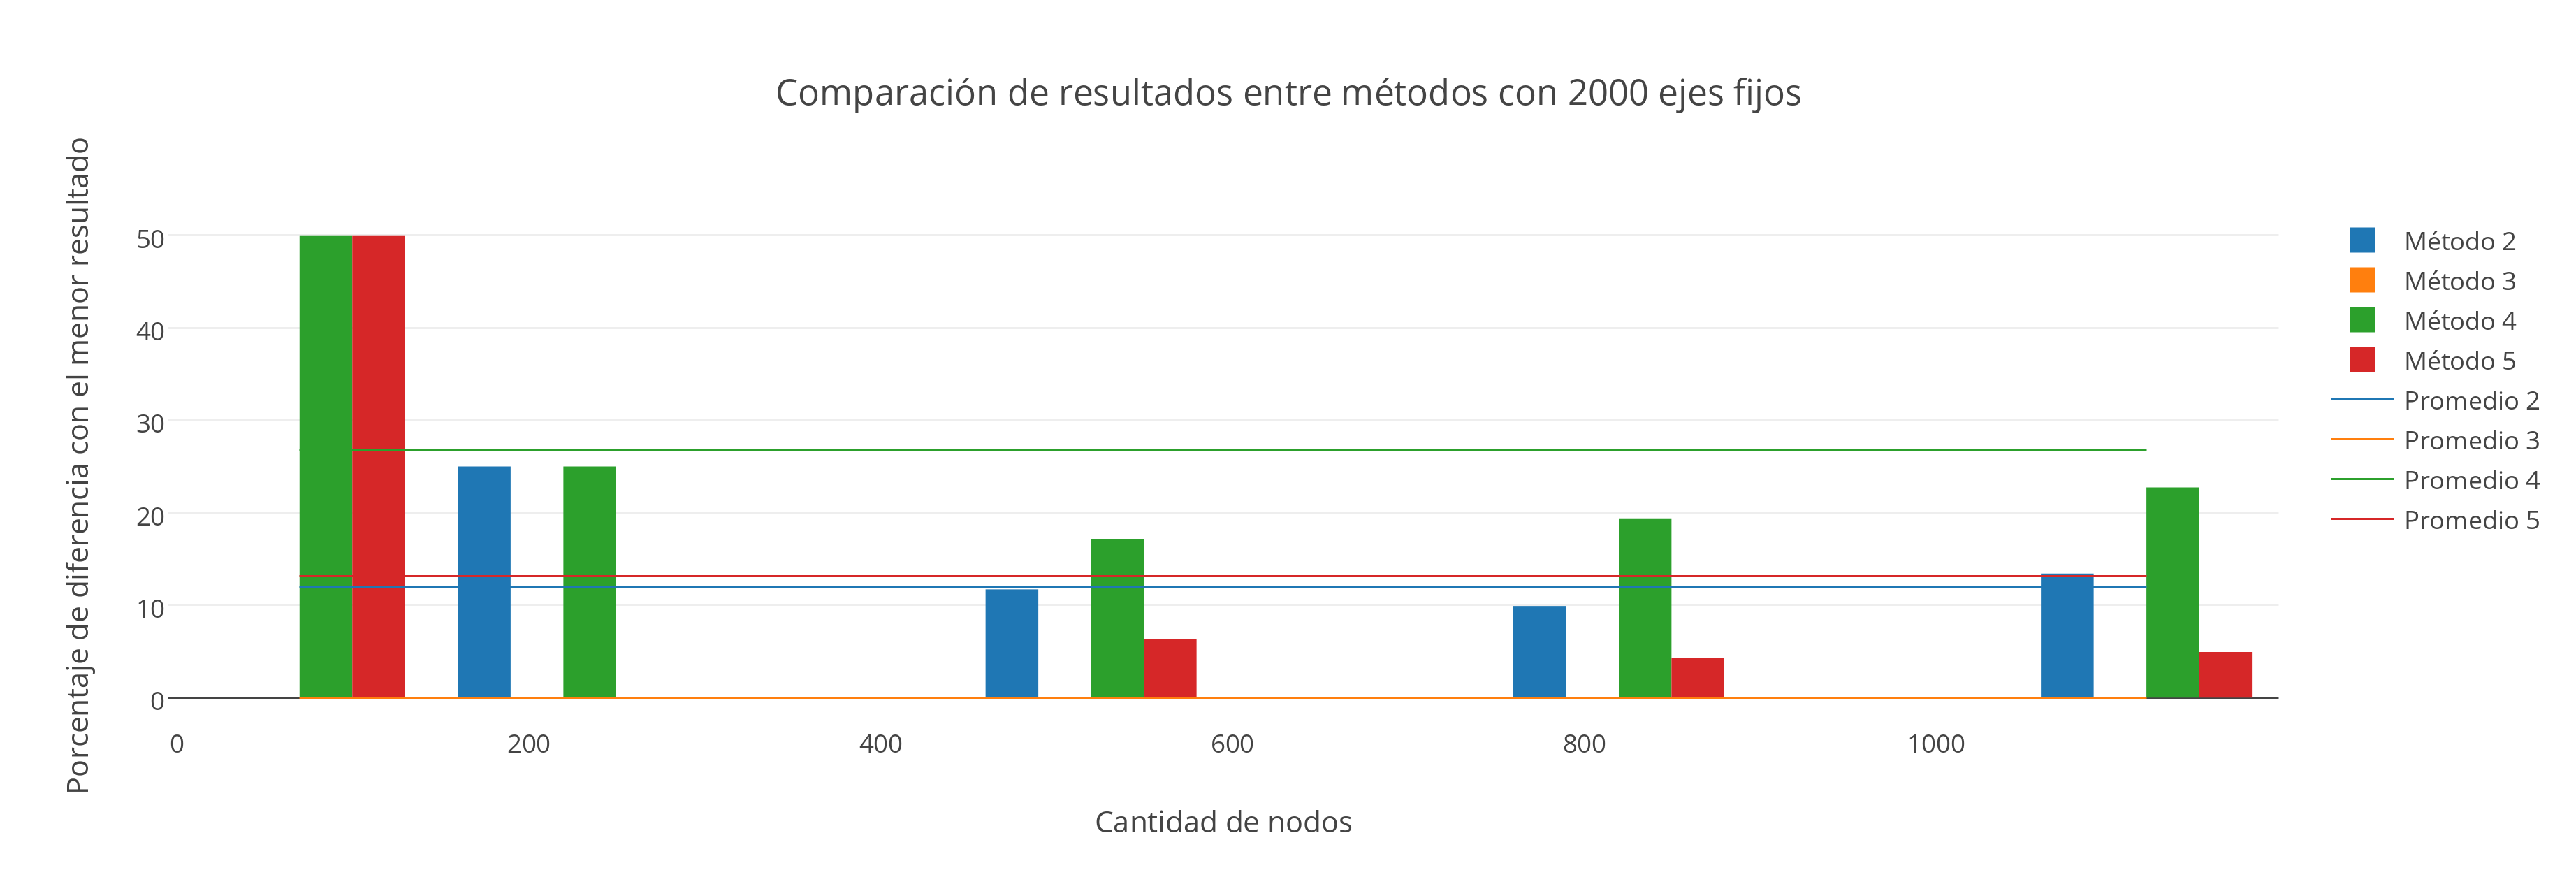
\includegraphics[scale=0.55]{imagenes/local/resultados/2000ejes.png}
% 	\caption{}
%	\label{10Nodos}
   \end{center}
 \end{figure}
 
  
\newpage  
  
\subsubsection*{Nodos Fijos}

  \begin{figure}[h!]
   \begin{center}
 	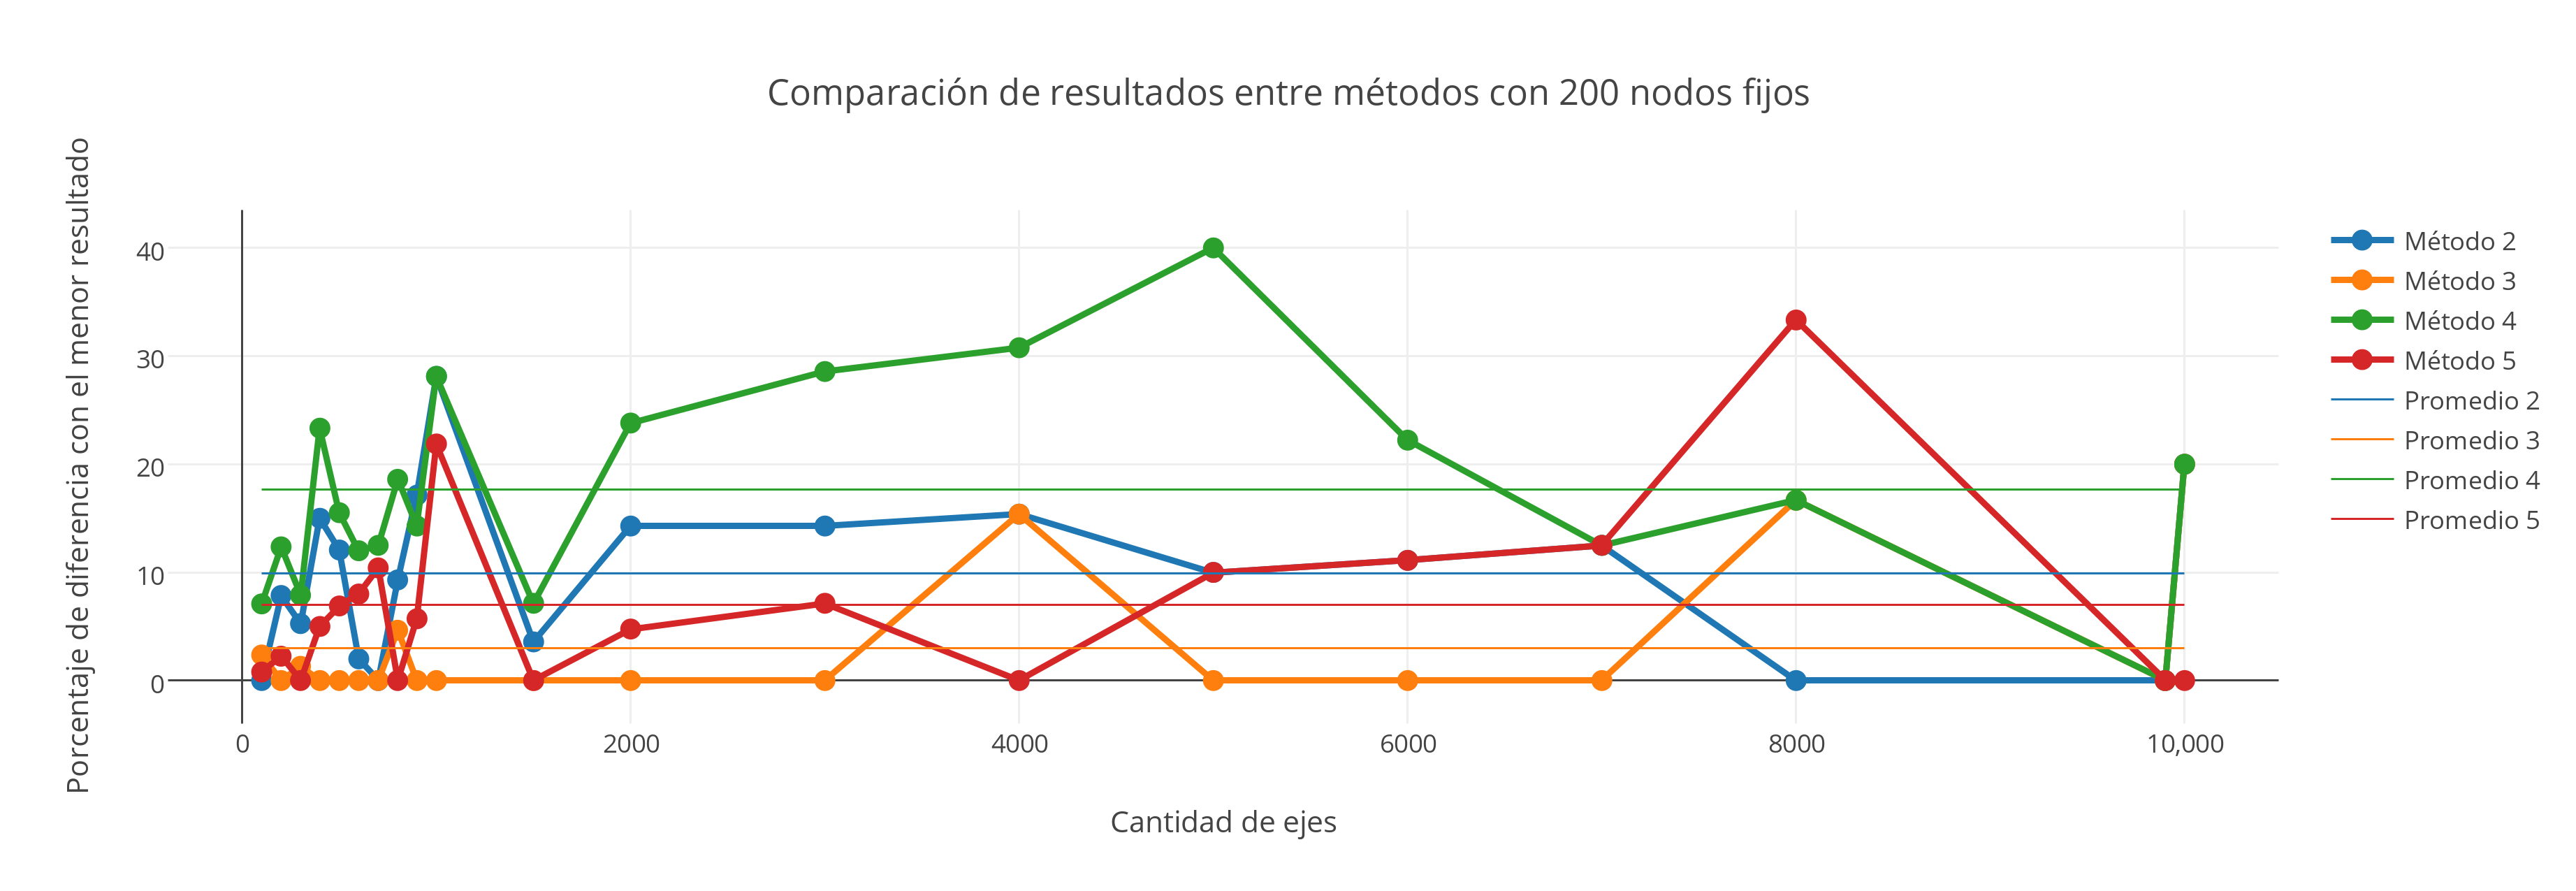
\includegraphics[scale=0.55]{imagenes/local/resultados/200nodos.png}
% 	\caption{}
%	\label{10Nodos}
   \end{center}
 \end{figure}
 
  \begin{figure}[h!]
   \begin{center}
 	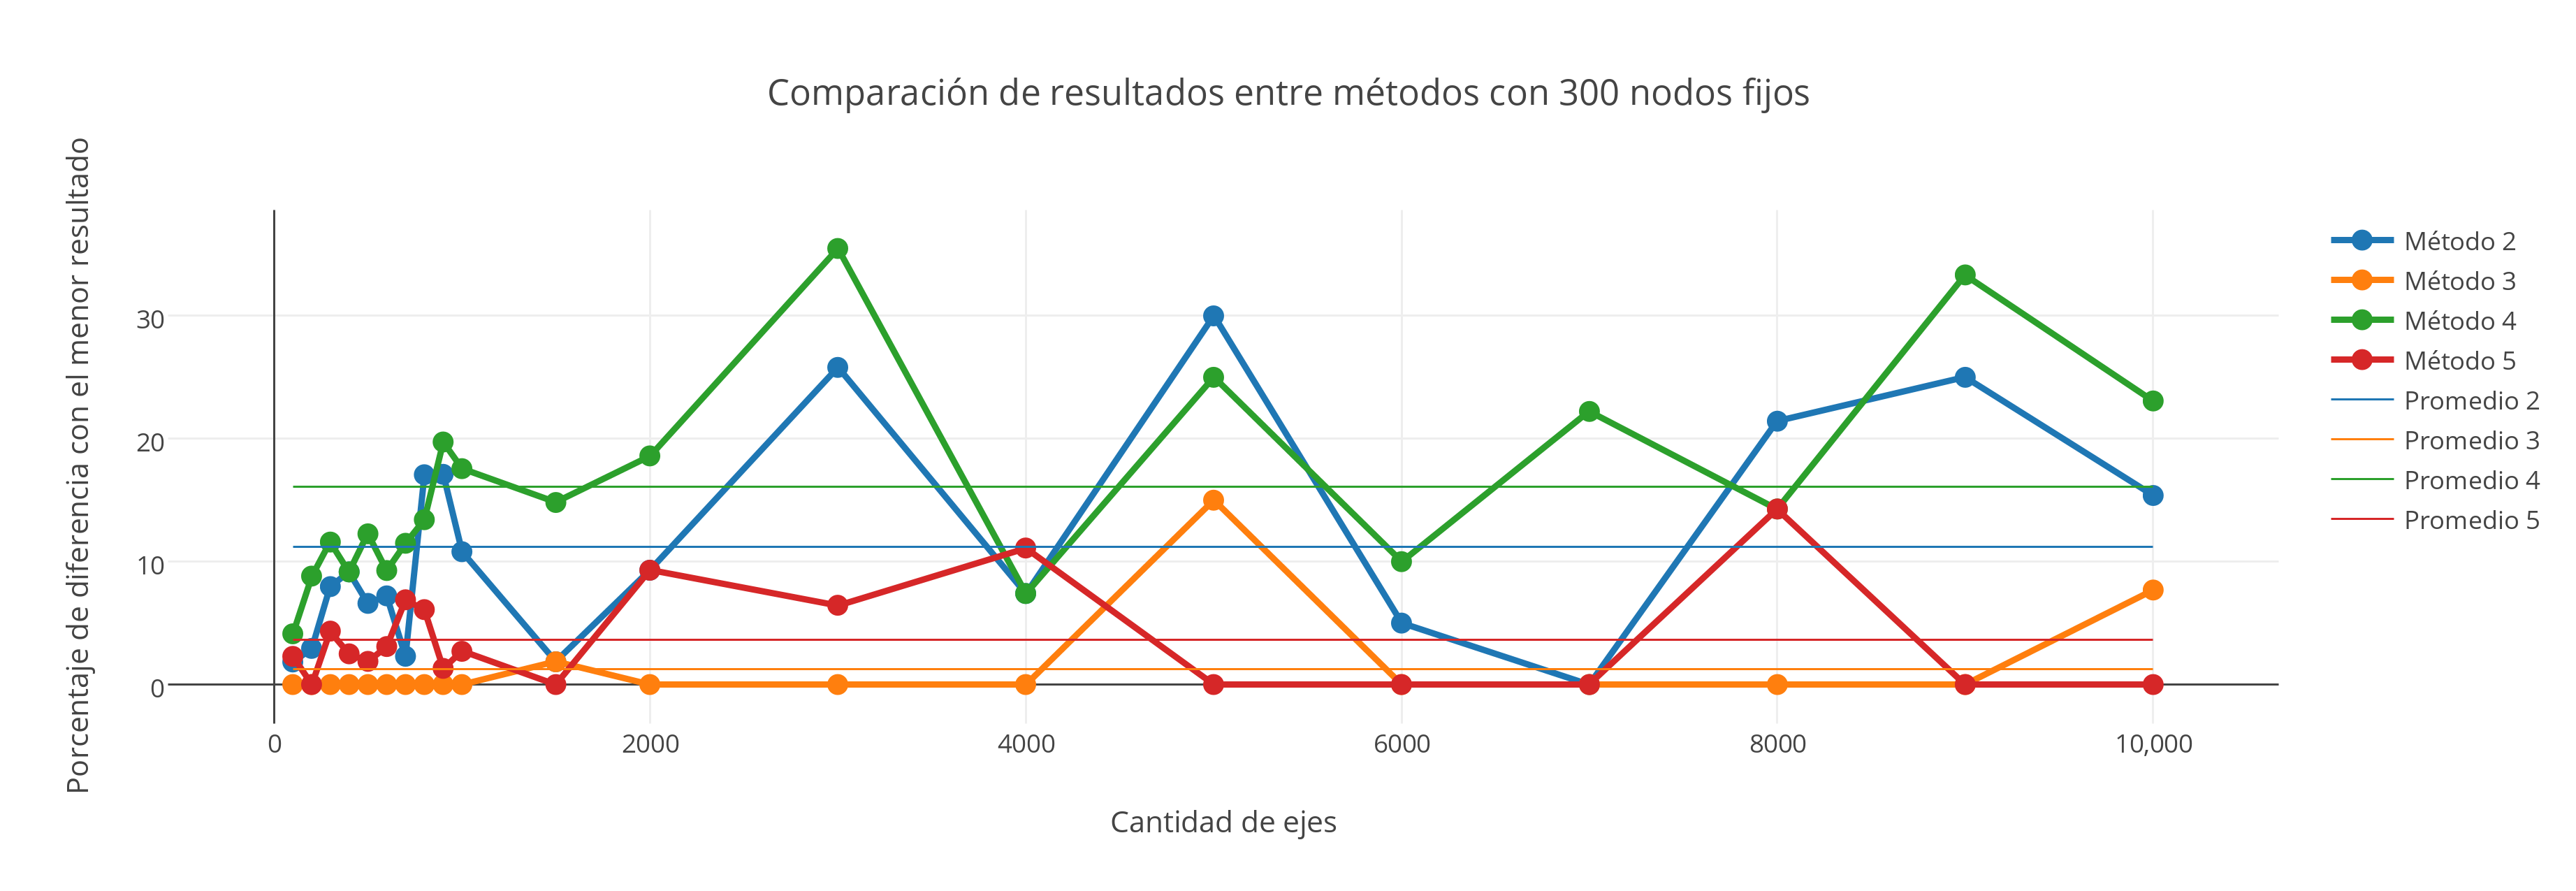
\includegraphics[scale=0.55]{imagenes/local/resultados/300nodos.png}
% 	\caption{}
%	\label{10Nodos}
   \end{center}
 \end{figure}
 

  \begin{figure}[h!]
   \begin{center}
 	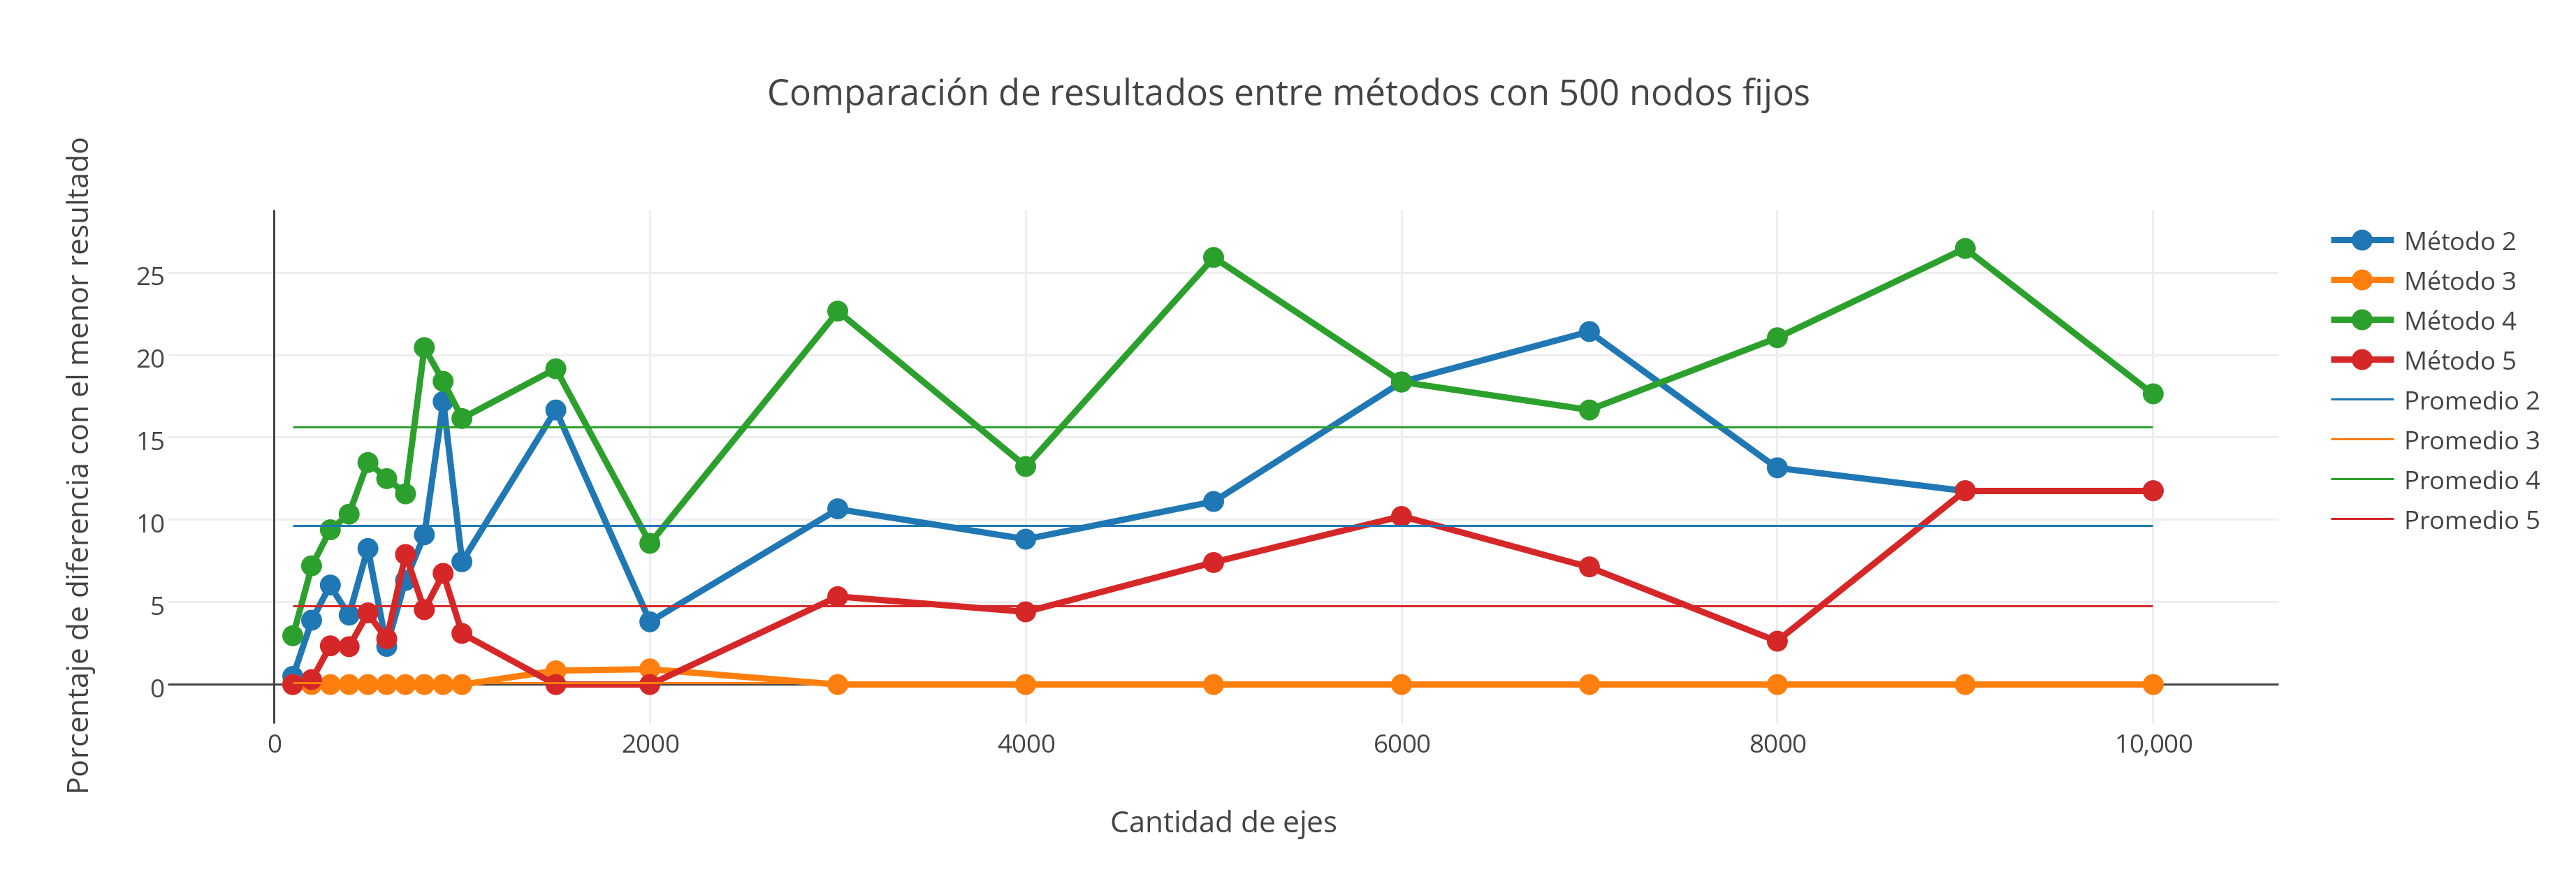
\includegraphics[scale=0.55]{imagenes/local/resultados/500nodos.png}
% 	\caption{}
%	\label{10Nodos}
   \end{center}
 \end{figure}
 
 \newpage
   \begin{figure}[h!]
   \begin{center}
 	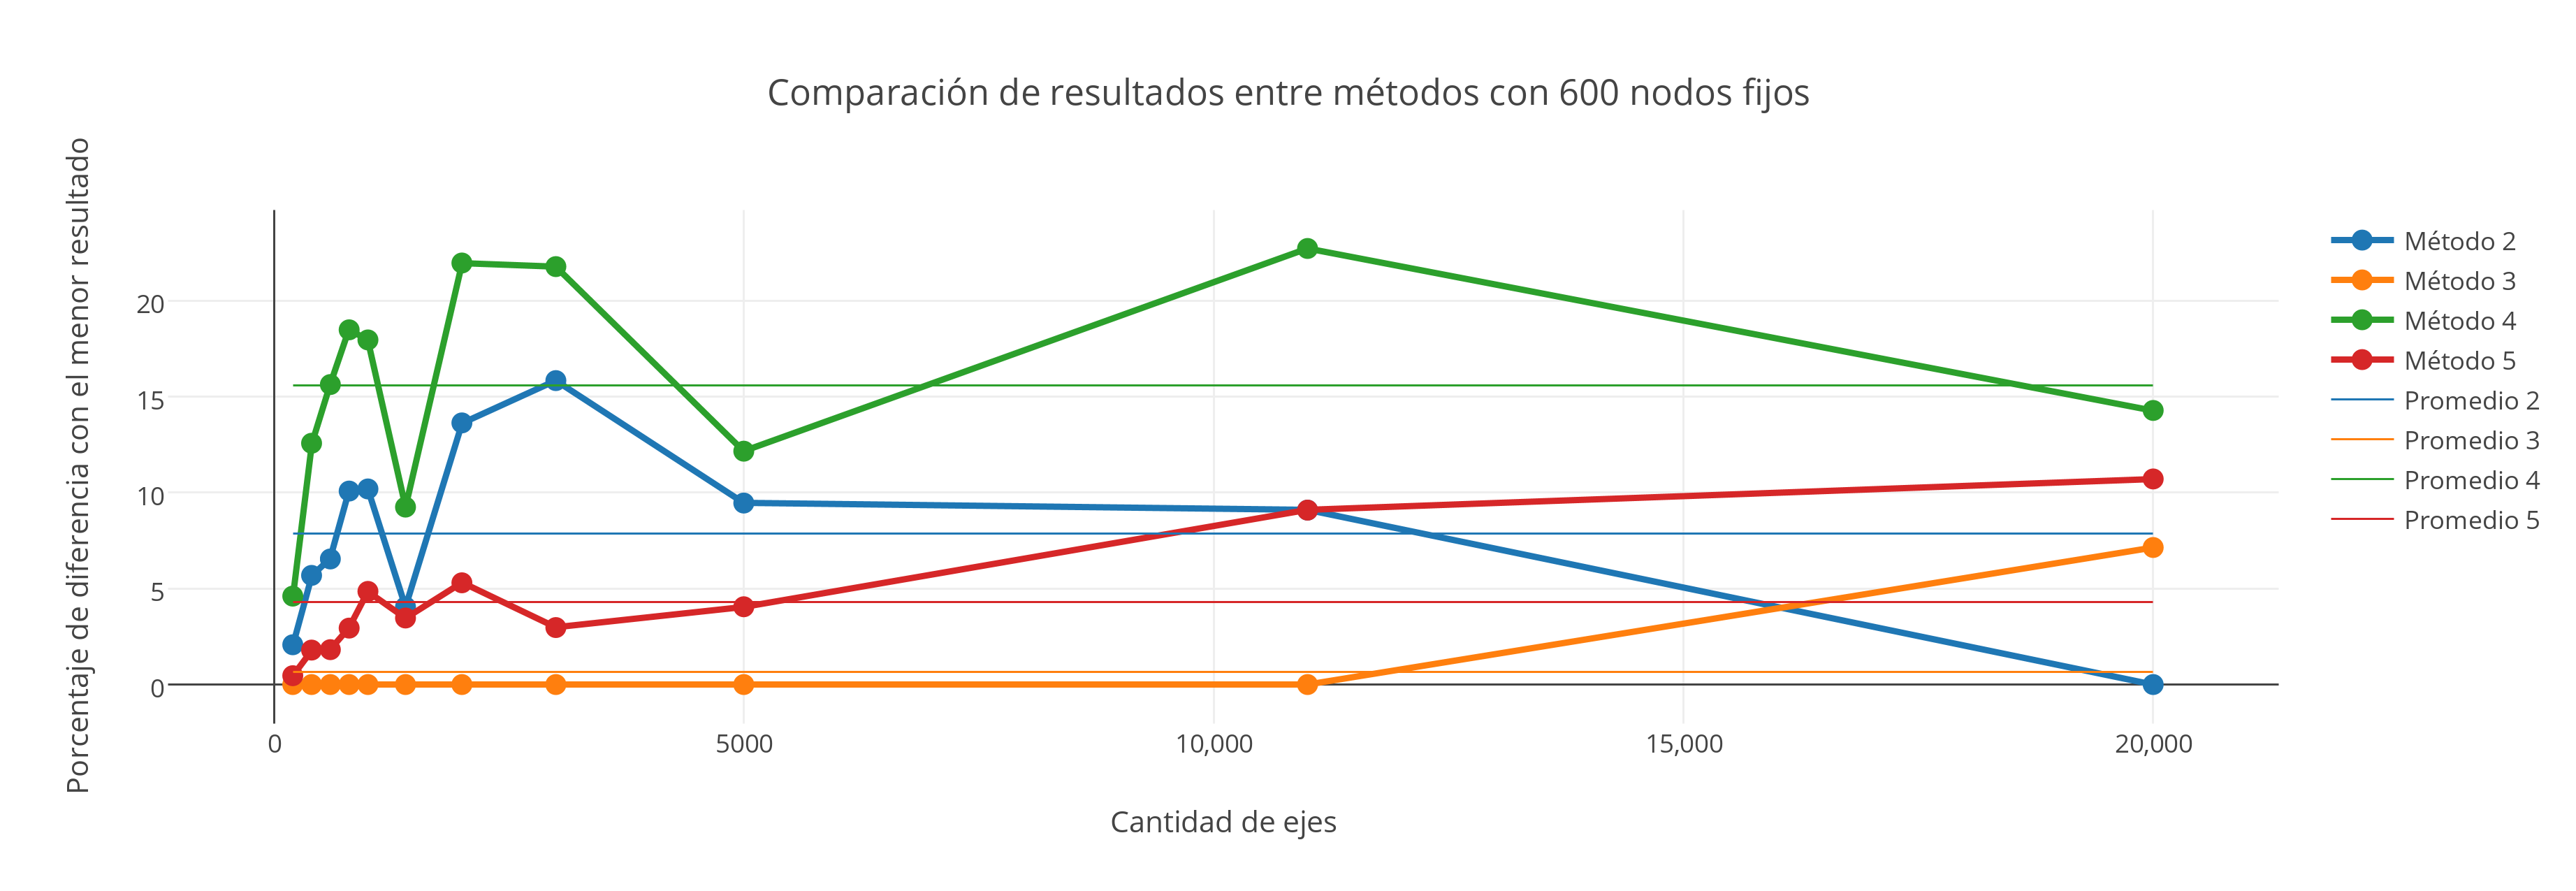
\includegraphics[scale=0.55]{imagenes/local/resultados/600nodos.png}
% 	\caption{}
%	\label{10Nodos}
   \end{center}
 \end{figure}

  \begin{figure}[h!]
   \begin{center}
 	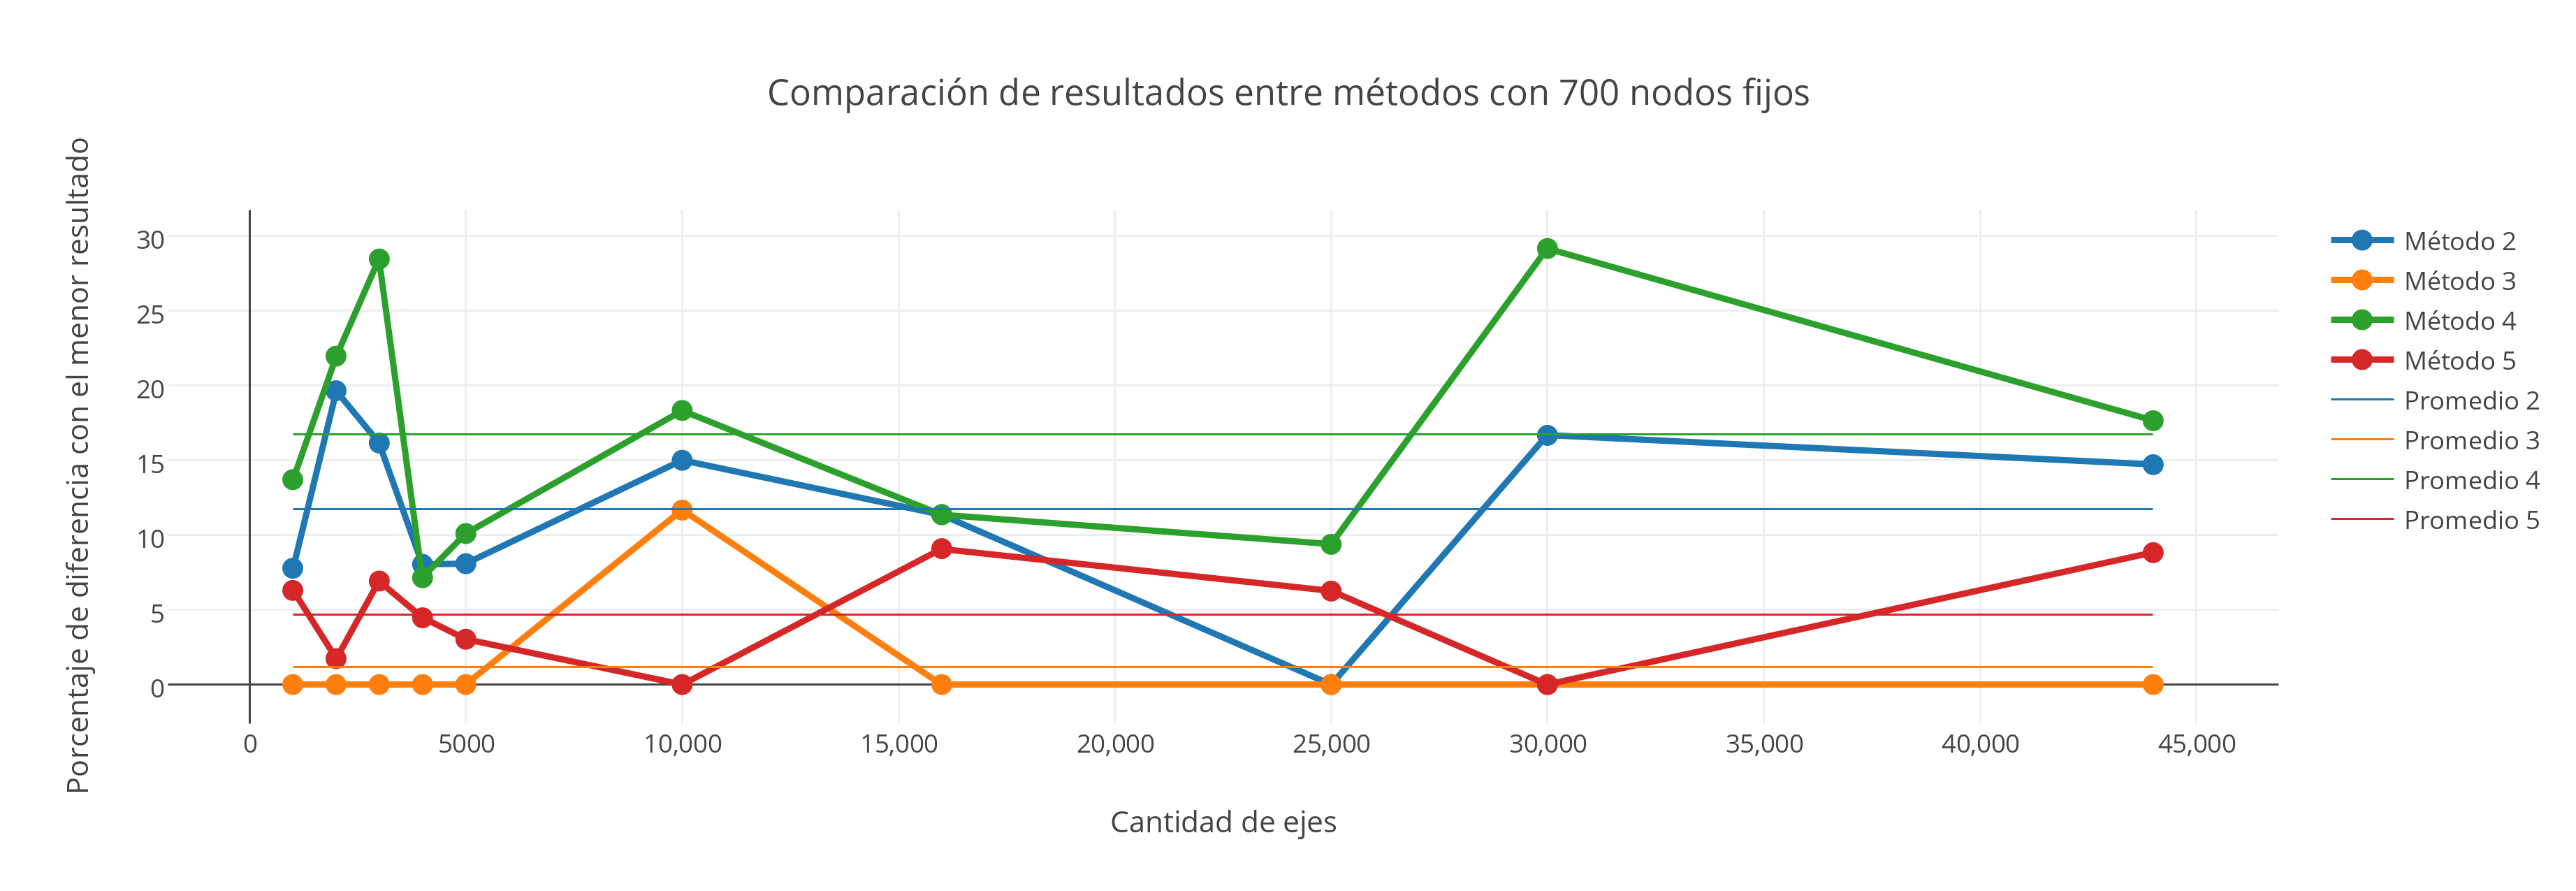
\includegraphics[scale=0.55]{imagenes/local/resultados/700nodos.png}
% 	\caption{}
%	\label{10Nodos}
   \end{center}
 \end{figure} 


\newpage
\newpage
%\section{Metaheur\'istica GRASP}
\subsection{Explicaci\'on}
La metaheur\'istica GRASP (Greedy Randomized Adaptive Search Procedure), es una mezcla de las dos heur\'isticas previas, dicho de manera simple, genera un punto de partida de forma golosa para el algoritmo de b\'usqueda local. Pero la distinci\'on se logra en como se construye "golosamente" la soluci\'on inicial:

Como la sigla lo indica, es un Goloso Randomizado, es decir que se escogen candidatos a soluci\'on inicial de forma golosa, pero en vez de elegir al que mejor resultados nos pueda arrojar, elegimos alguno de los que mejor lo har\'a. Particularmente optamos por elegir un nodo entre los $\alpha$\% mejores.

Entonces, si nuestro grafo tiene un nodo de grado m\'aximo mayor estricto a los dem\'as, no necesariamente lo elegiremos.

Luego se aplica el algoritmo de b\'usqueda local explicado en el inciso anterior sin modificaciones.

Un aspecto tambi\'en diferencial de esta heur\'istica, es que no generamos una \'unica instancia inicial, sino que se toman un n\'umero arbitrario de ellas (seg\'un el criterio de parada) y guardamos la soluci\'on \'optima que encontramos, si en alg\'un momento se mejora, se actualiza.

La RCL (Restricted Candidate List) var\'ia seg\'un el $alpha$ elegido (si se elige 0, ser\'a un greedy), a mayor $alpha$, mayor diversidad de candidatos iniciales.

Las vecindades utilizadas son las mismas que se usan en la heur\'isitca de b\'usqueda local.

El criterio de parada que adoptamos fue el de llegar a una determina cantidad de repeticiones del algoritmo, b\'usqueda de soluci]'on inicial y b\'usqueda local a partir de ella, tal que la respuesta \'optima encontrada, no se viera modificada durante todas ellas.

%Explicar detalladamente el algoritmo implementado. Plantear distintos criterios de parada y de seleccion de la lista de candidatos (RCL) de la heurıstica golosa aleatorizada.
\subsection{Experimentaci\'on}
%Realizar una experimentacion que permita observar los tiempos de ejecucion y la calidad de las soluciones obtenidas. Se debe experimentar variando los valores de los parametros de la metaheurıstica (lista de candidatos, criterios de parada, etc.) y las vecindades utilizadas en la busqueda local. Elegir, si es posible, la configuracion que mejores resultados provea para el grupo de instancias utilizado.

\newpage
%\section{Comparaci\'on entre todos los m\'etodos} \label{ej6}

Una vez elegidos los mejores valores de configuracion para cada heurıstica implementada (si fue posible), realizar una experimentacion sobre un conjunto nuevo de instancias para observar la performance
de los metodos comparando nuevamente la calidad de las soluciones obtenidas y los tiempos de ejecucion en funcion de los parametros de la entrada. 
Para los casos que sea posible, comparar tambien los resultados del algoritmo exacto implementado.
Presentar todos los resultados obtenidos mediante graficos adecuados y discutir al respecto de los mismos.
\subsection{Resultados}
\subsubsection{Nodos fijos}
Aqu\'i se comparan los resultados de los 3 algoritmos (Grasp, Greedy y Local), manteniendo los nodos fijos. Nuestros tests fueron con nodos fijos desde 100 hasta 1000 y para cada una de esas instancias,
variando los ejes de a 100, comenzando con 1000 ejes.\\

En estos gr\'aficos, vamos a buscar, para cada cambio en los ejes, cu\'al fue el que menos nodos utiliza en su respuesta. \'Este ser\'a el mejor en cuanto a resultados.\\

Mostraremos los gr\'aficos con 100, 300, 600 y 900 nodos fijos:

\begin{center}
 	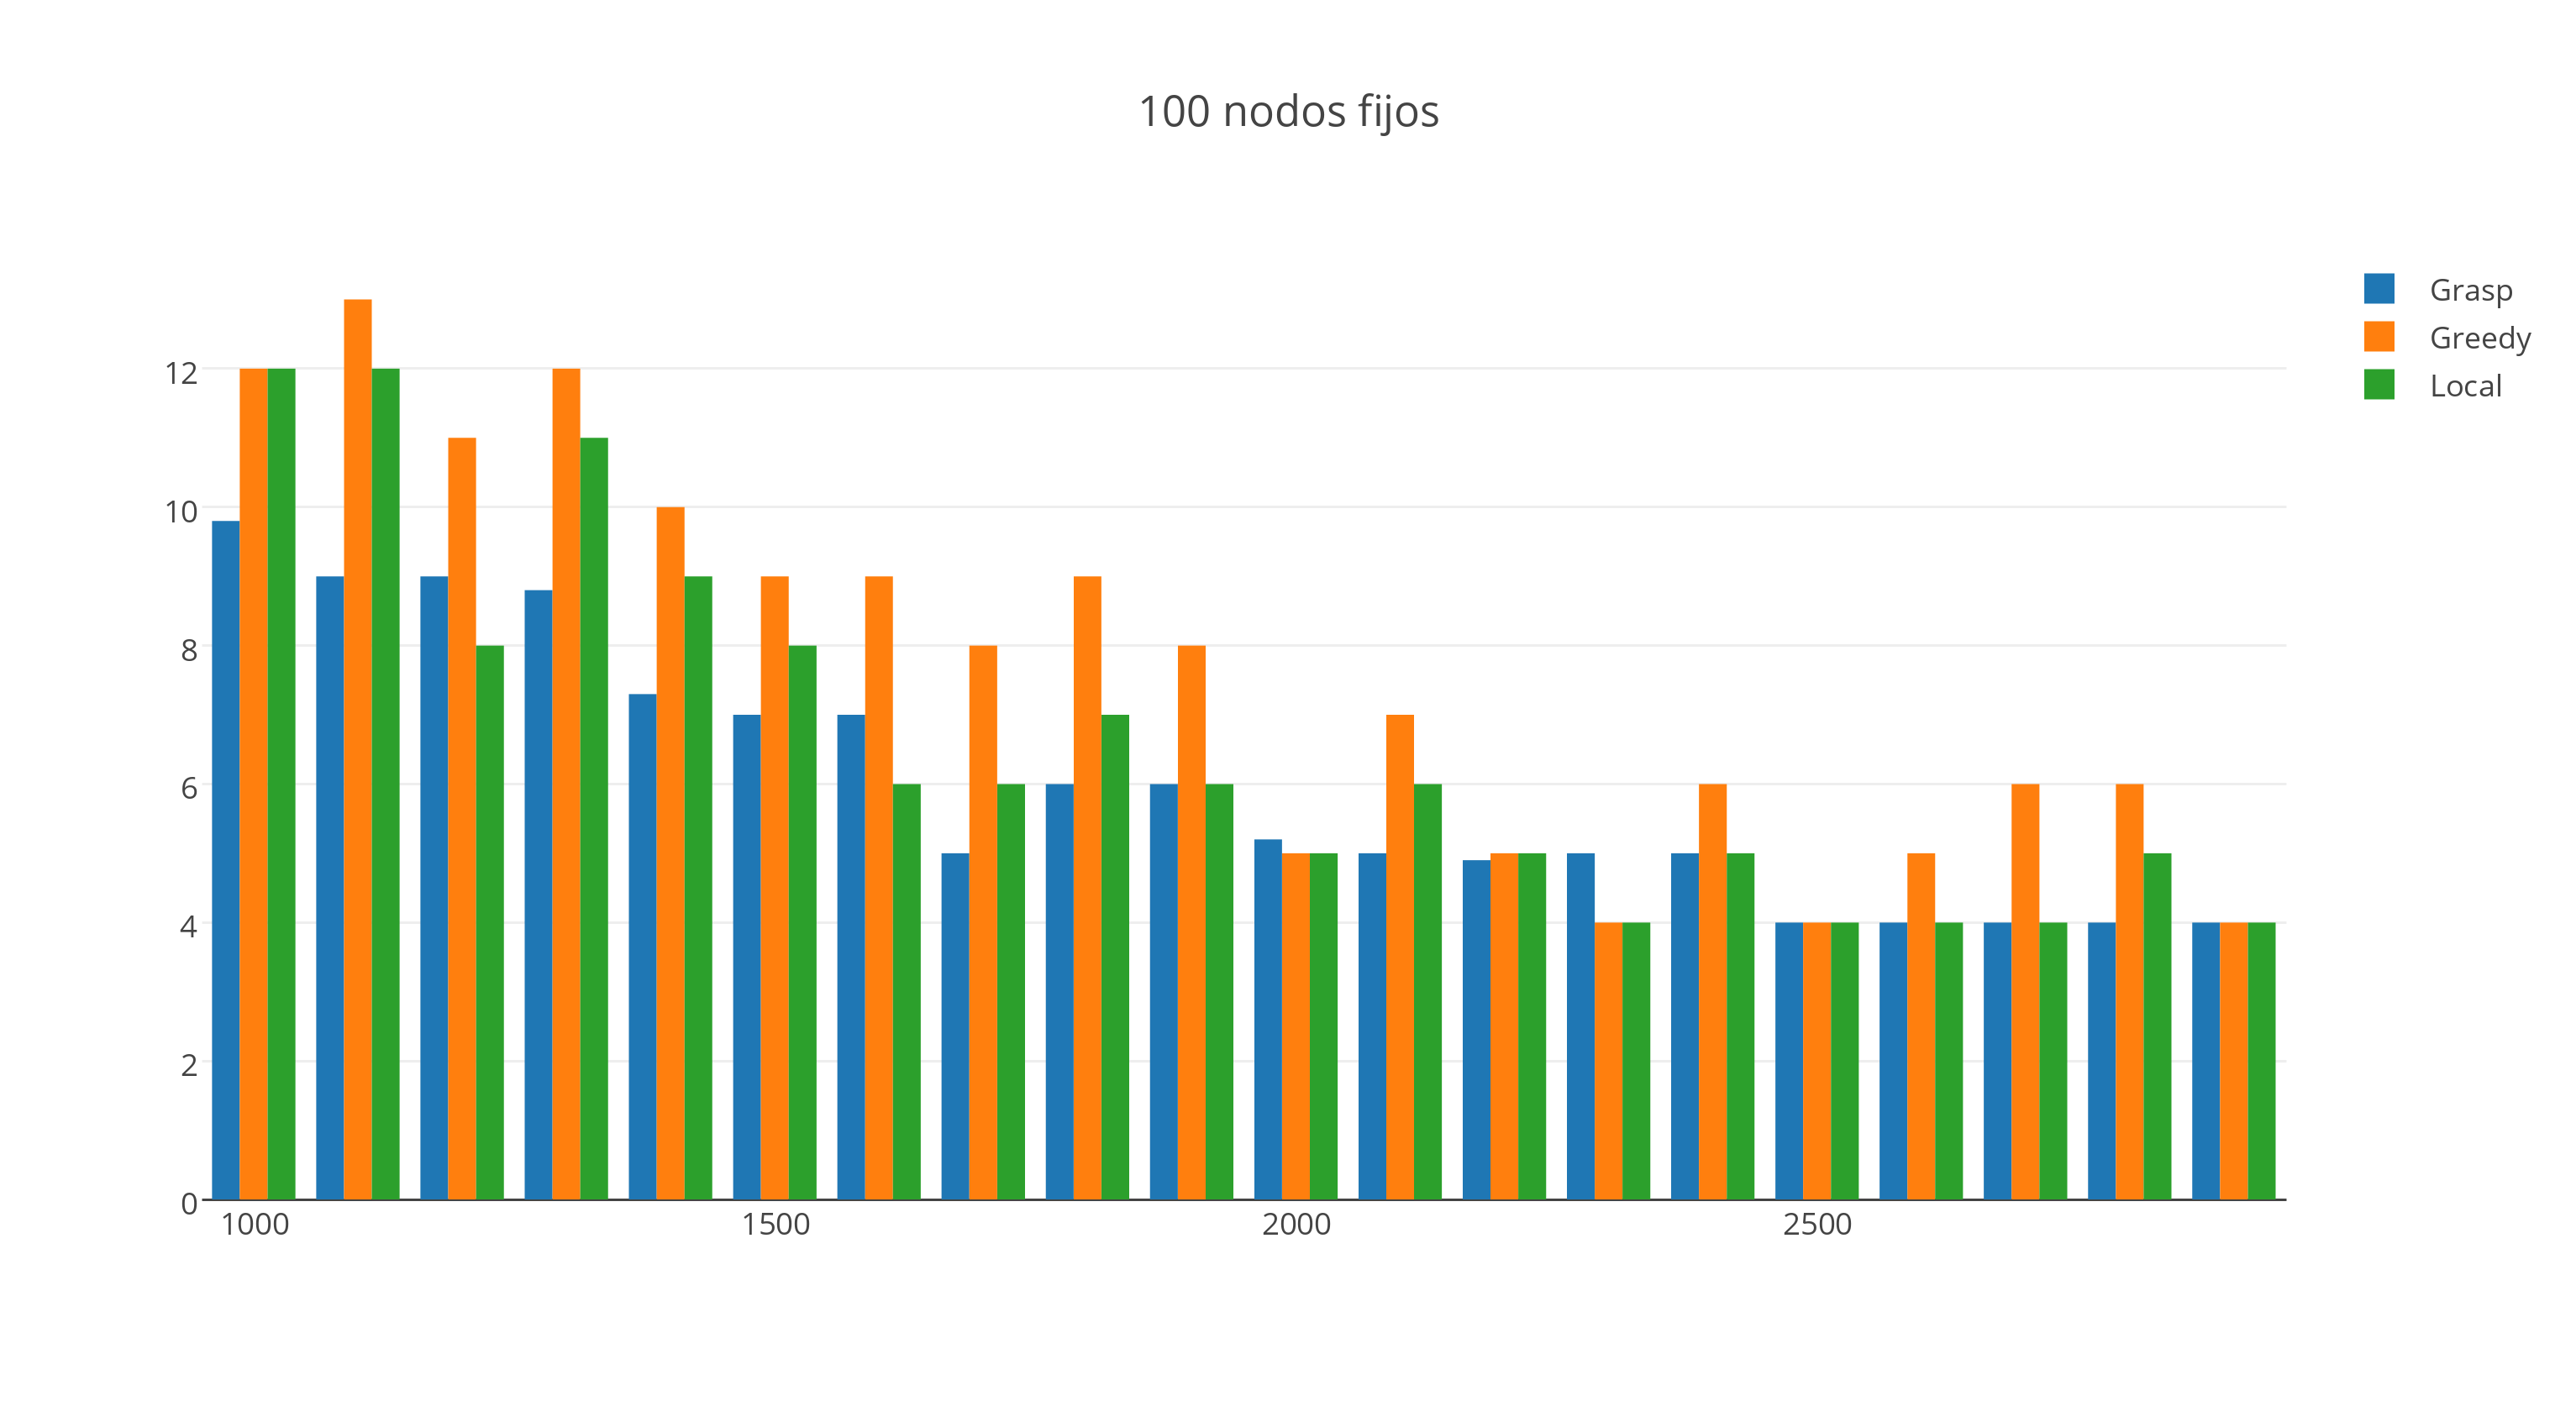
\includegraphics[width=13cm, keepaspectratio=yes]{imagenes/6/100NodosFijos.png}

 	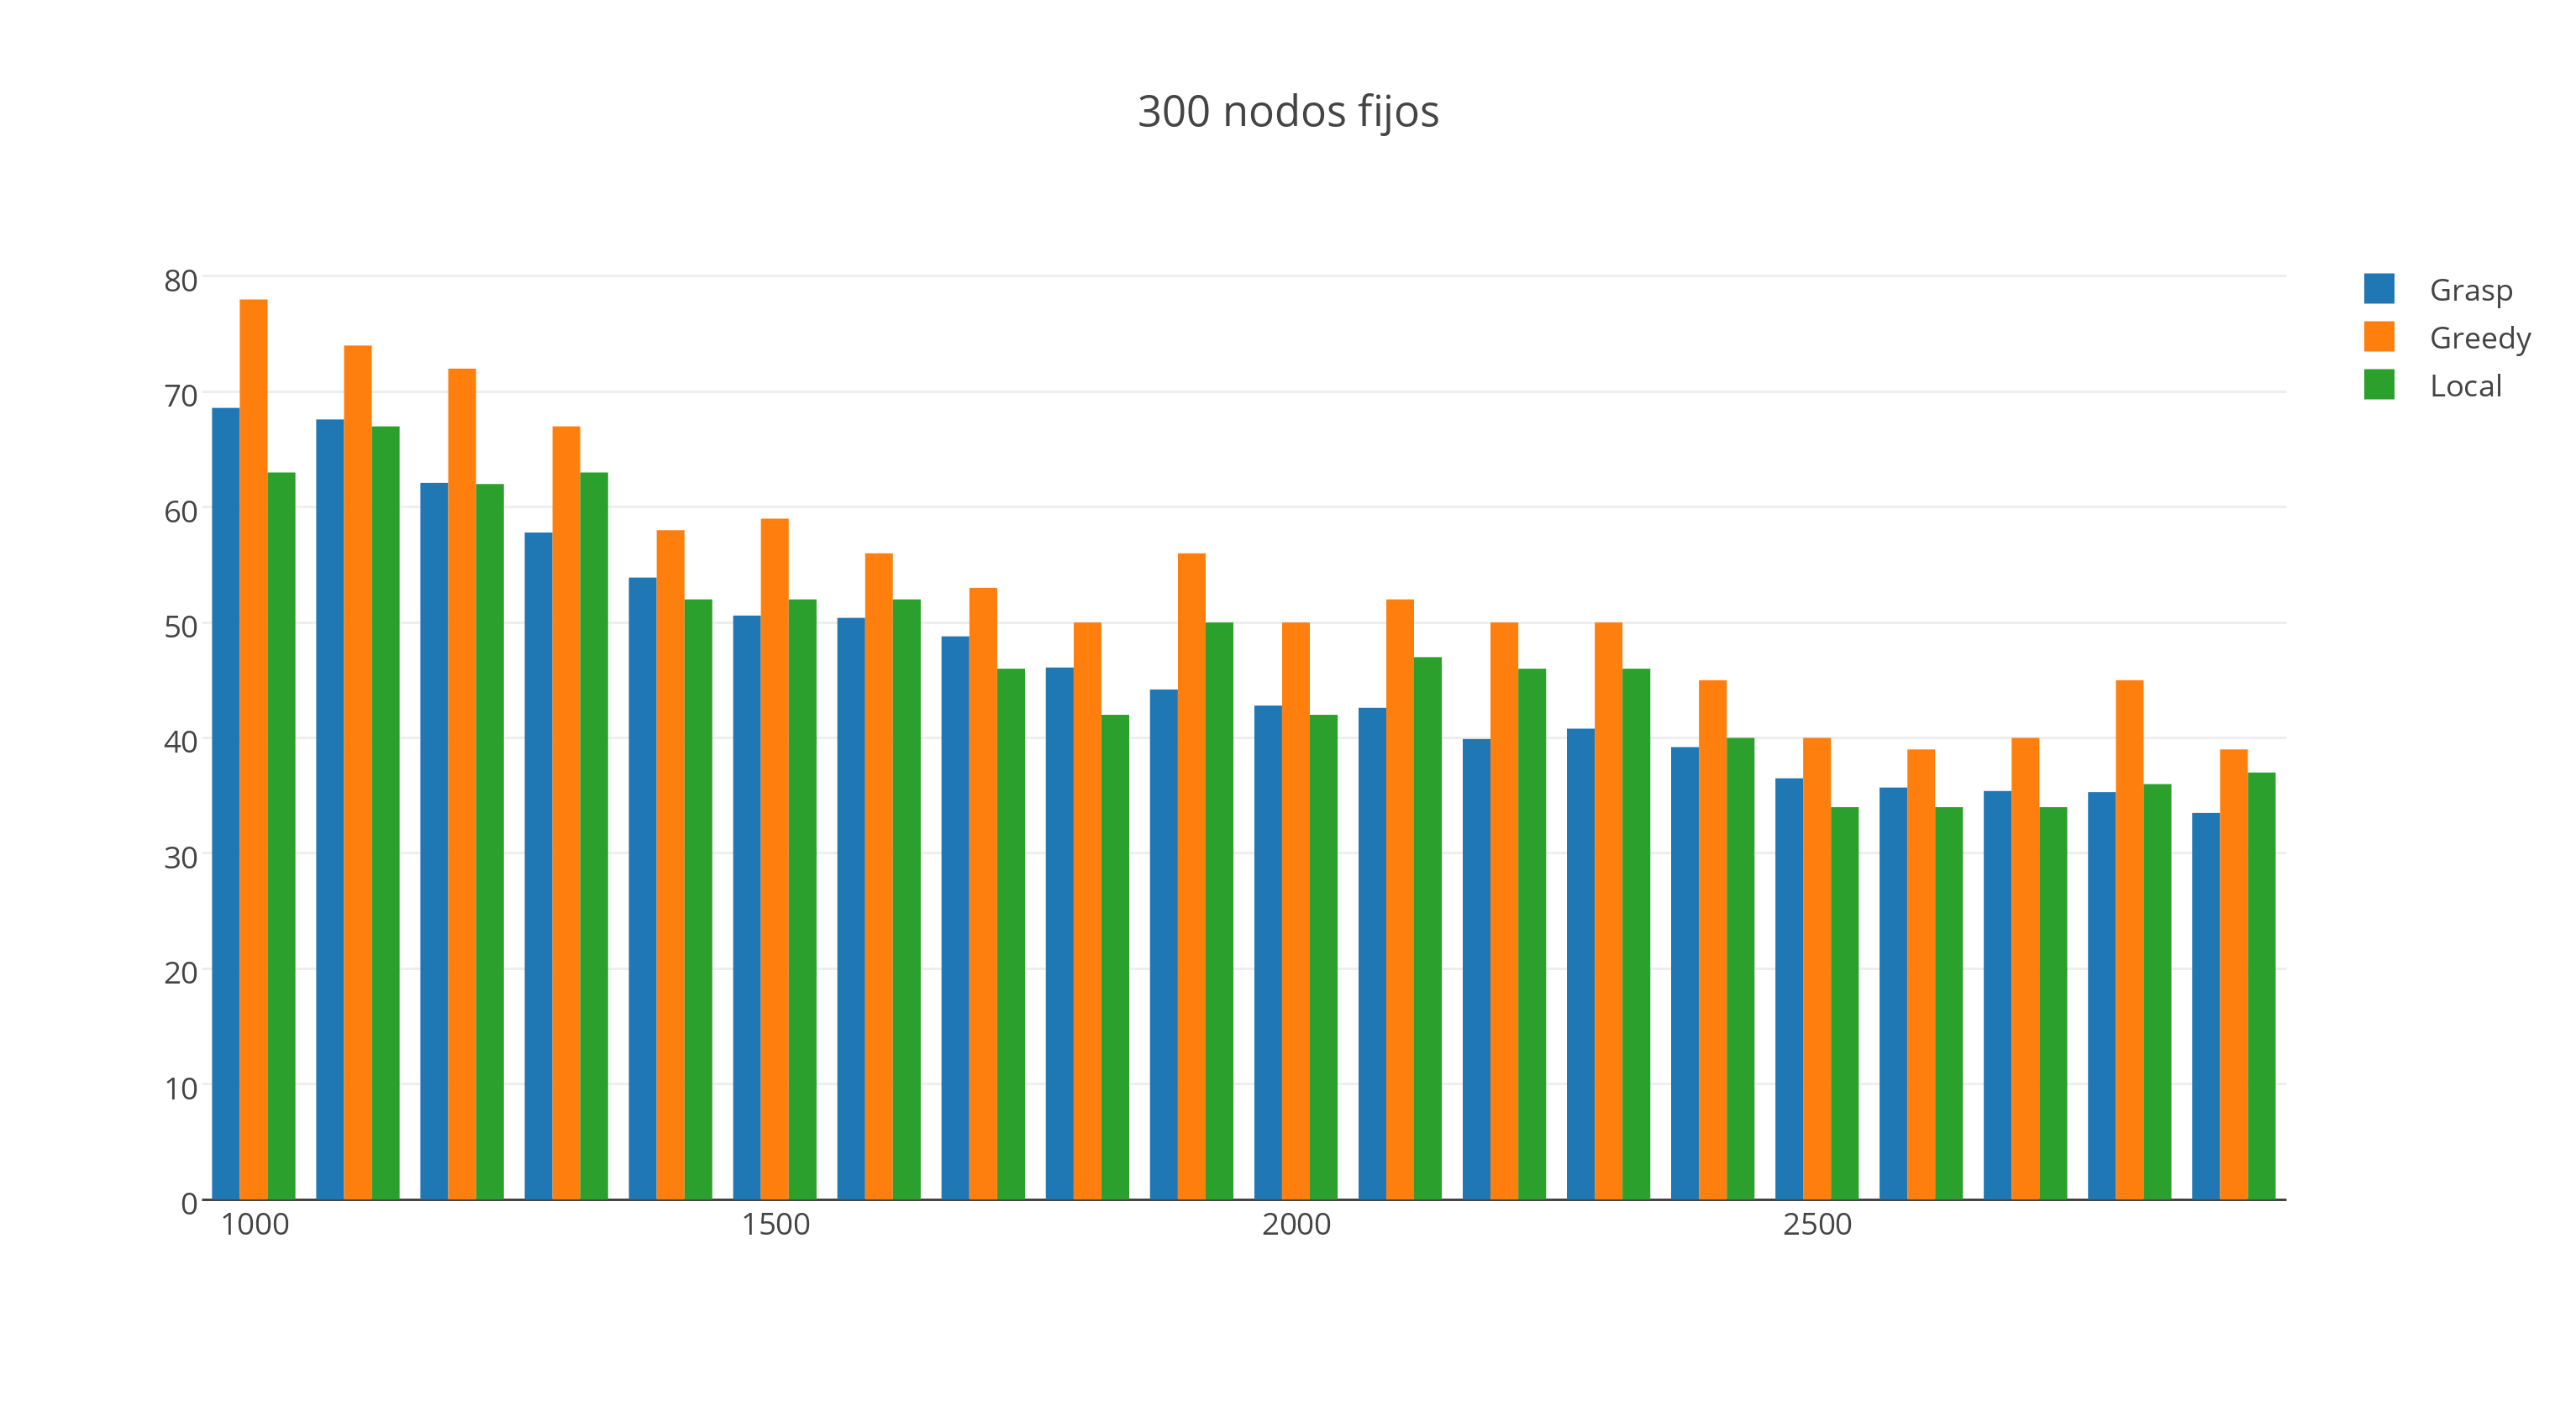
\includegraphics[width=13cm, keepaspectratio=yes]{imagenes/6/300NodosFijos.png}
 
 	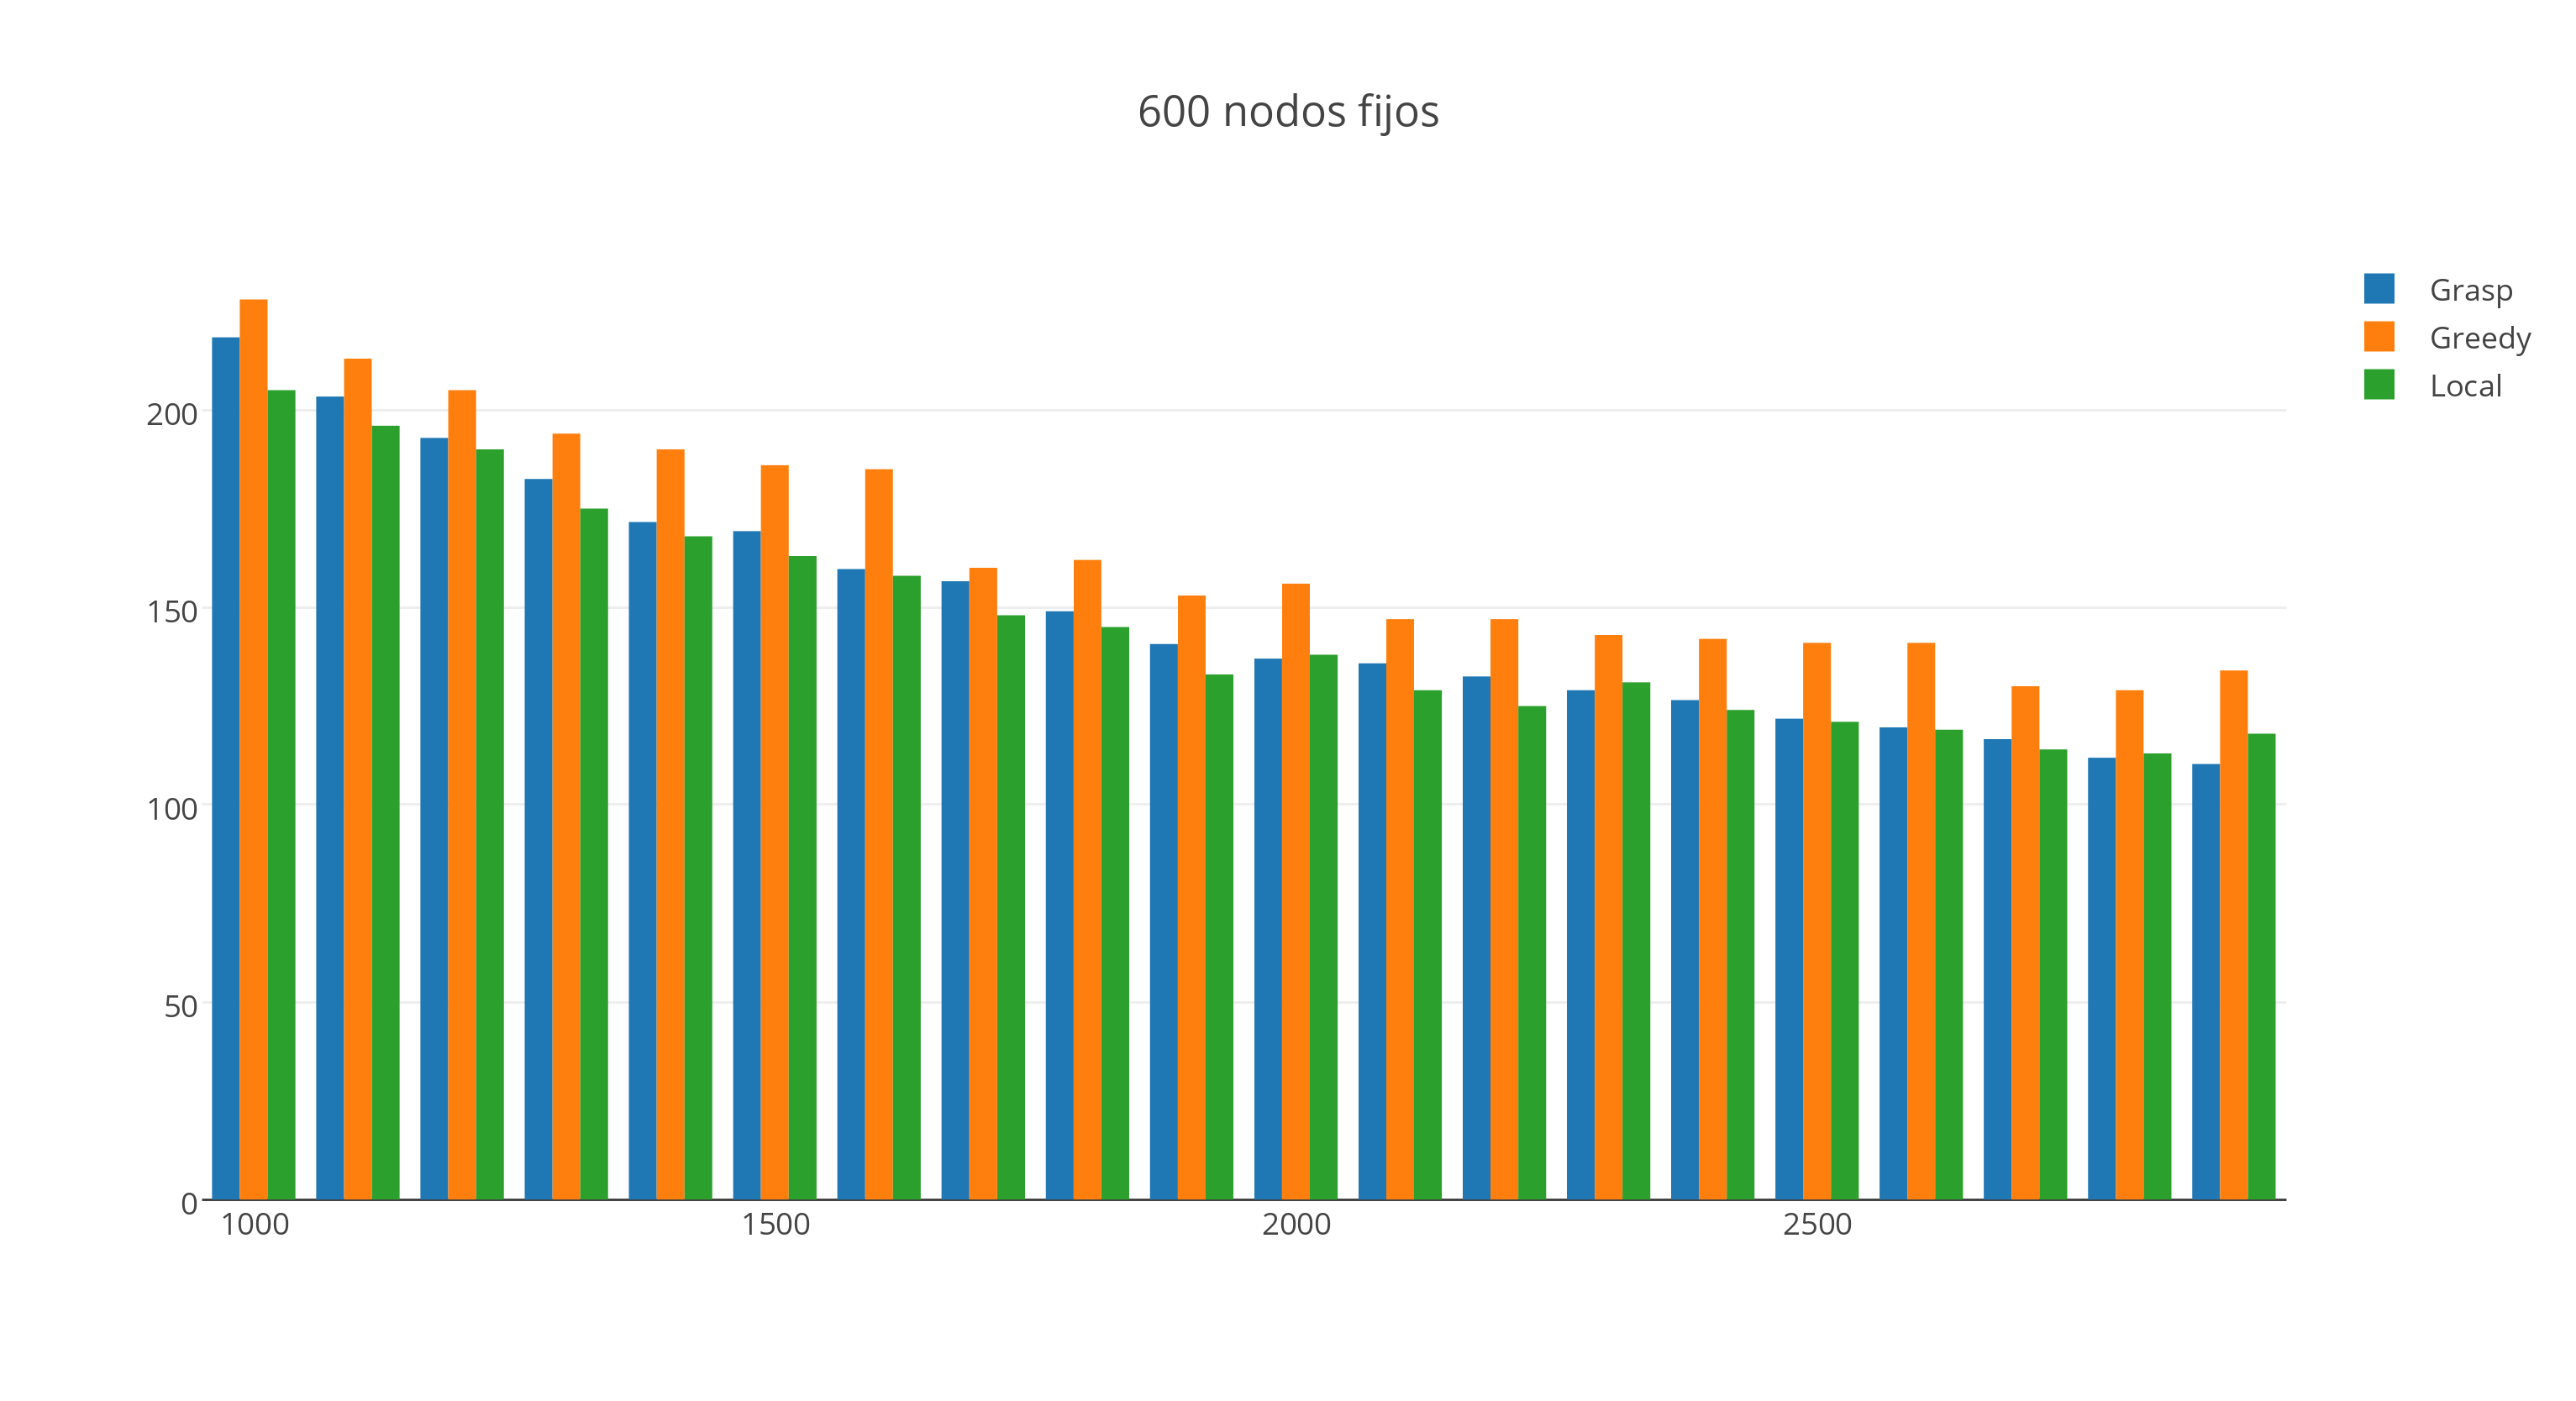
\includegraphics[width=13cm, keepaspectratio=yes]{imagenes/6/600NodosFijos.png}
 
 	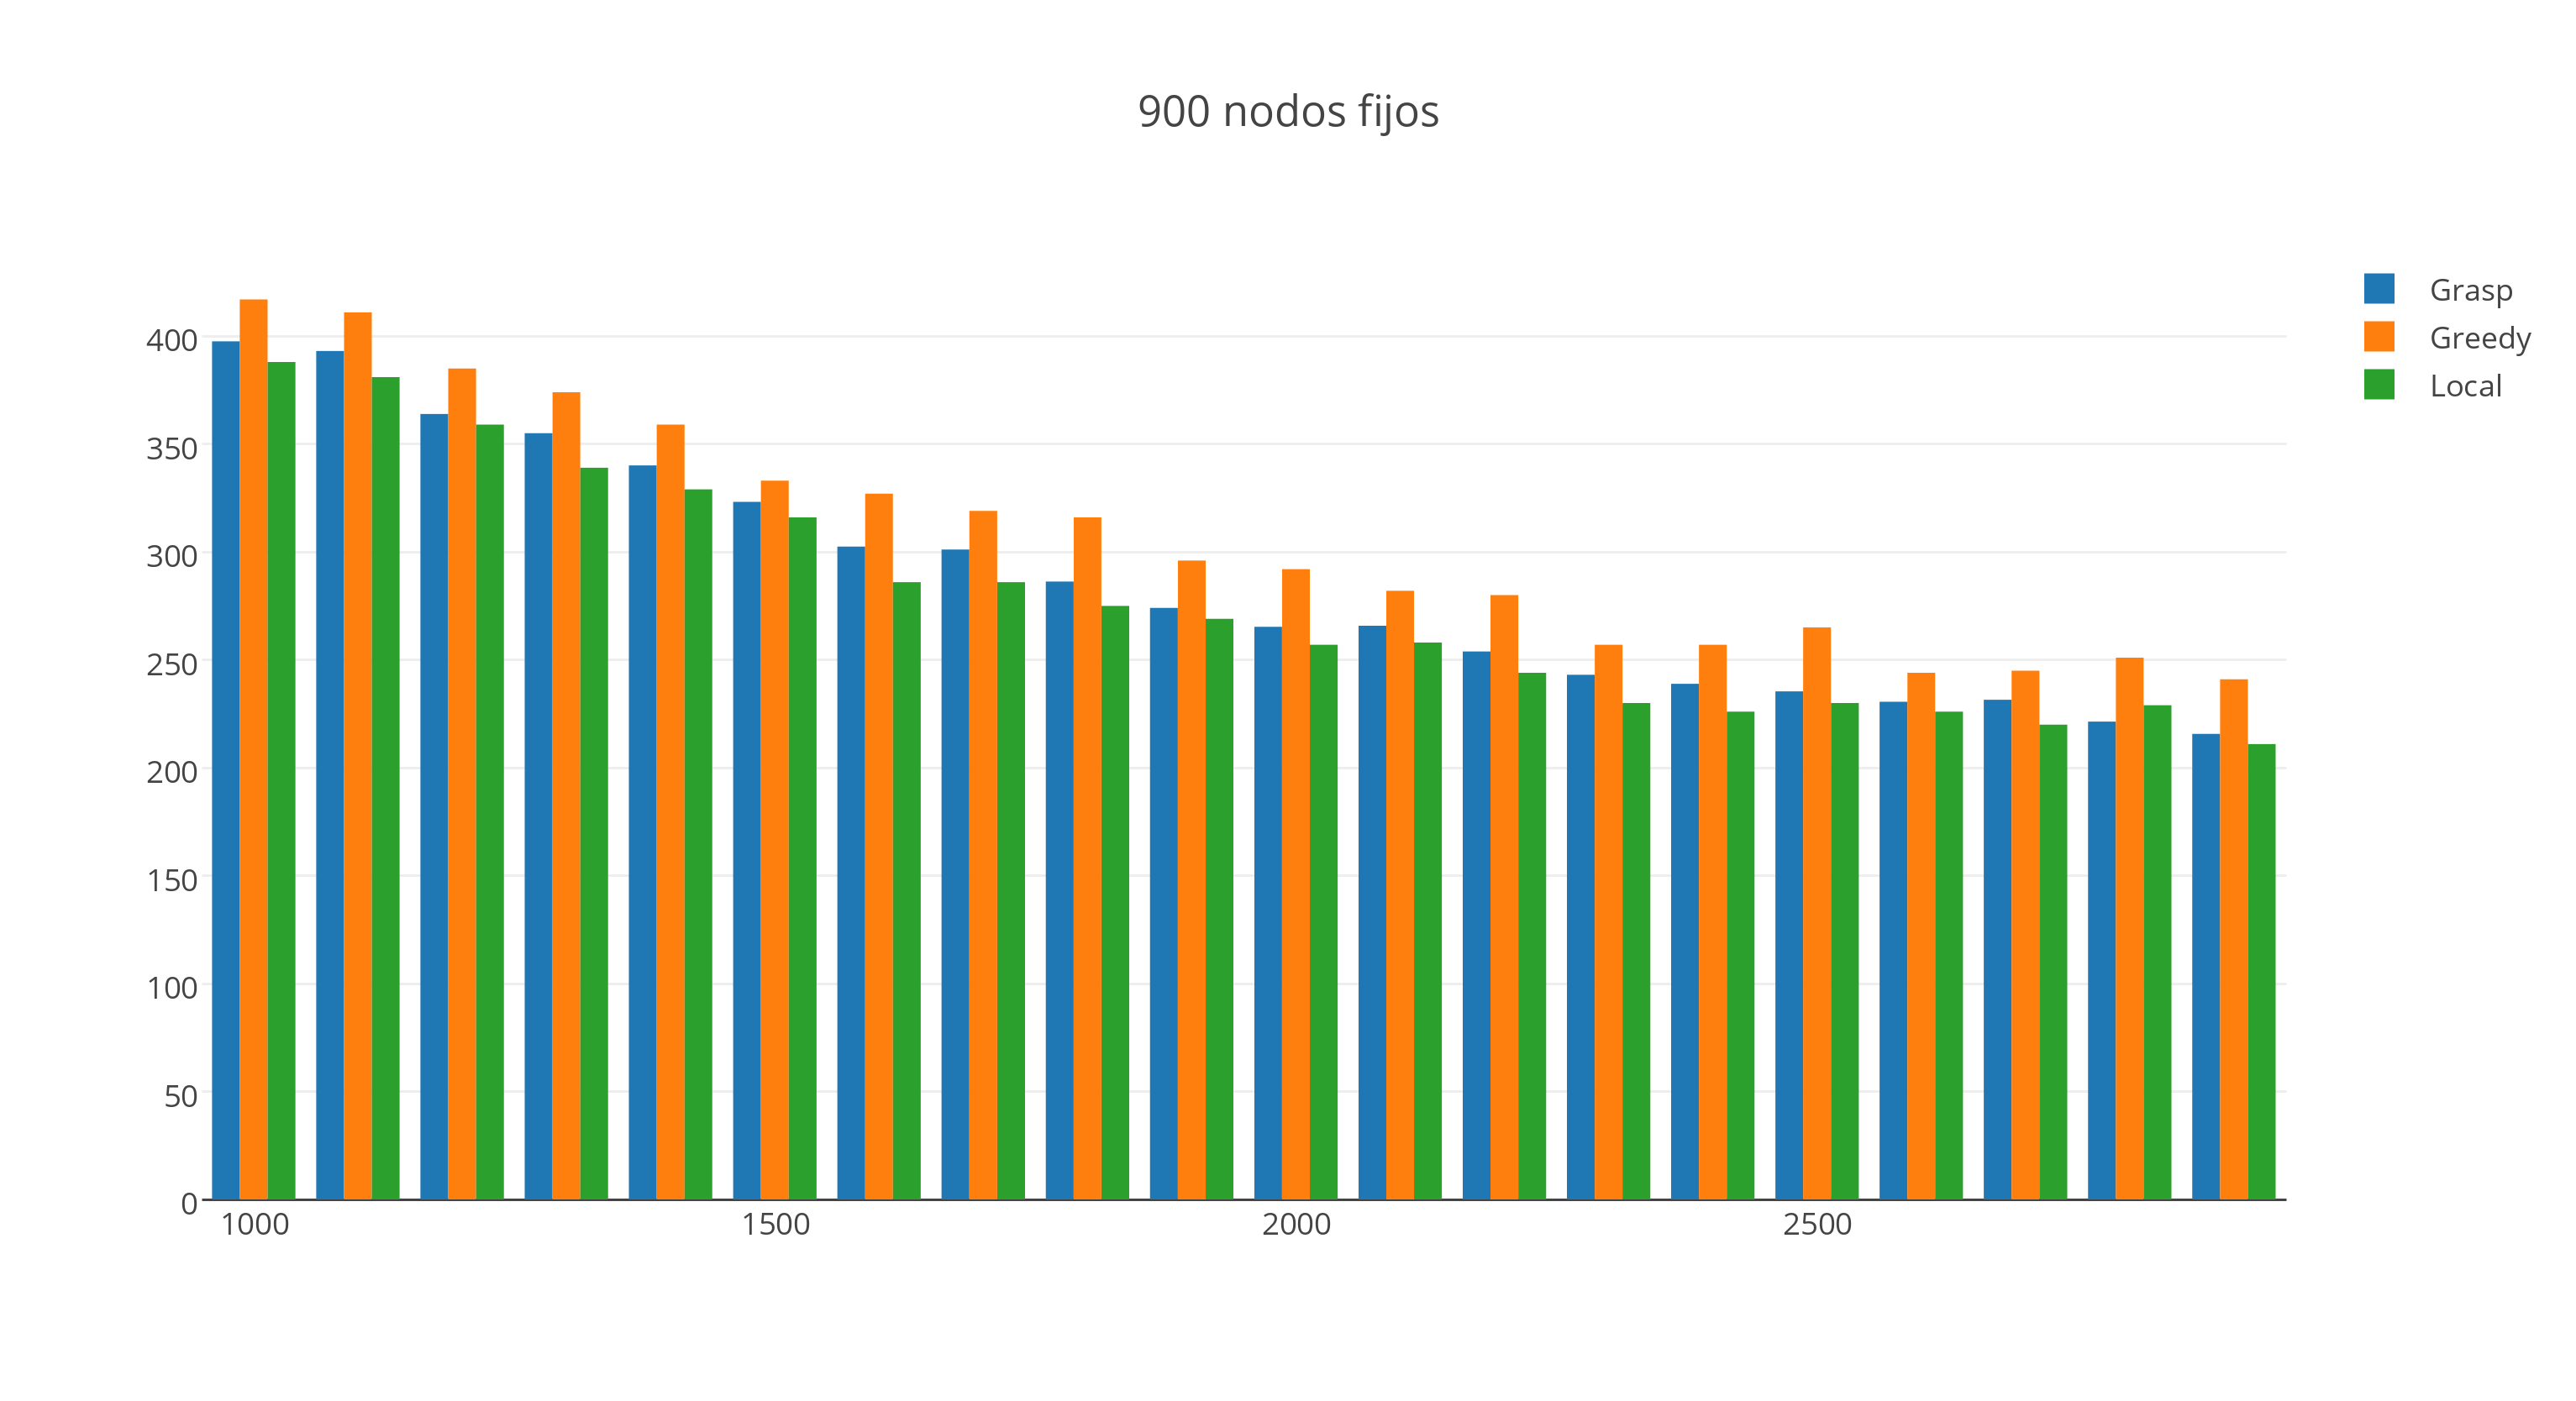
\includegraphics[width=13cm, keepaspectratio=yes]{imagenes/6/900NodosFijos.png}
\end{center}
 
Analizando estos gr\'aficos, podemos ver r\'apidamente que el algoritmo Greedy nos devuelve en todos los casos una soluci\'on peor que los otros dos, ya que utiliza mayor cantidad de nodos.\\
Por otra parte, se puede ver cierta ventaja del Grasp para los casos m\'as chicos (100, 300 nodos), pero para los casos grandes (600, 900 nodos), se ve que el Local es mejor en casi todos los casos.\\

No podemos distinguir claramente cu\'al es la mejor opci\'on entre estos dos, ya que los valores son bastante cambiantes a lo largo de los 4 gr\'aficos, por lo que buscamos el promedio de nodos que utiliza
cada algoritmo. Los resultados fueron los siguientes:\\

\begin{tabular}{| l | l | l | l |}
   \hline
   Nodos & Grasp & Local & Greedy\\ \hline
   100 & 6 & 6.55 & 7.65 \\ \hline
   300 & 46.59 & 47.25 & 53.65 \\ \hline
   600 & 149.255 & 145.65 & 164.3 \\ \hline
   900 & 289.925 & 277.95 & 307.55 \\
   \hline
\end{tabular}

Estos promedios confirman los datos que se pod\'ian apreciar en los gr\'aficos, es decir, que el Greedy utiliza siempre mayor cantidad de nodos que los otros, que Grasp es mejor en los casos chicos y
que a medida que crece la cantidad de nodos, es preferible el Local.\\

También se analizaron los tiempos de ejecución en las mismas instancias, cuyos resultados fueron los siguientes:

\begin{center}
 	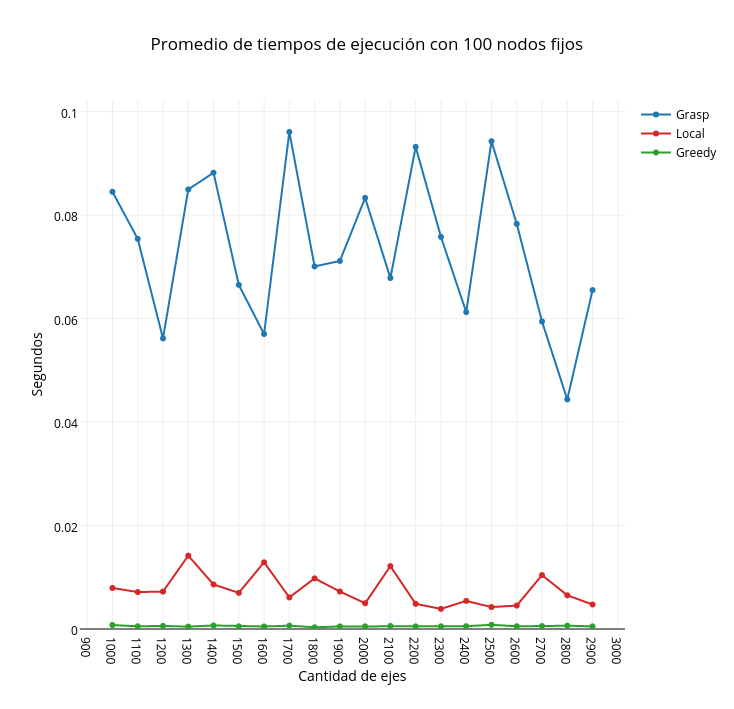
\includegraphics[width=13cm, keepaspectratio=yes]{imagenes/coliseo/Fixnode/100.png}

 	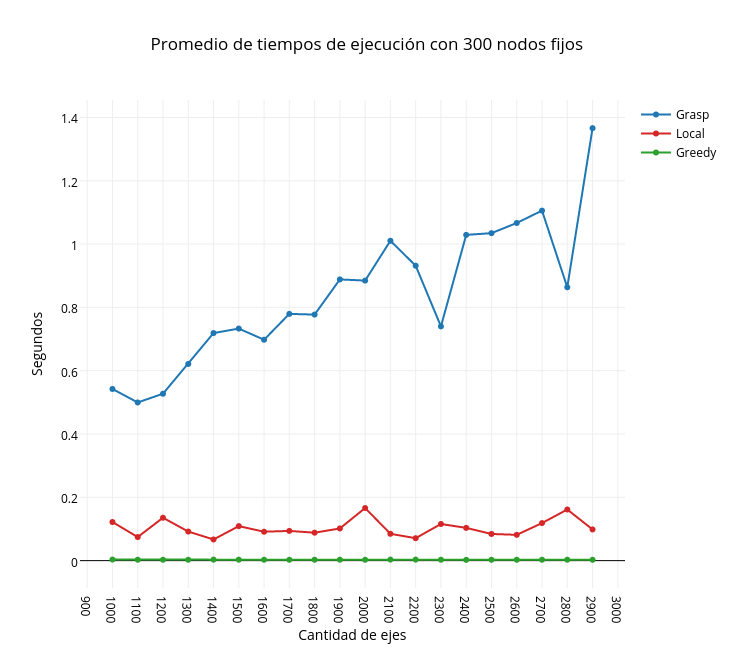
\includegraphics[width=13cm, keepaspectratio=yes]{imagenes/coliseo/Fixnode/300.png}

 	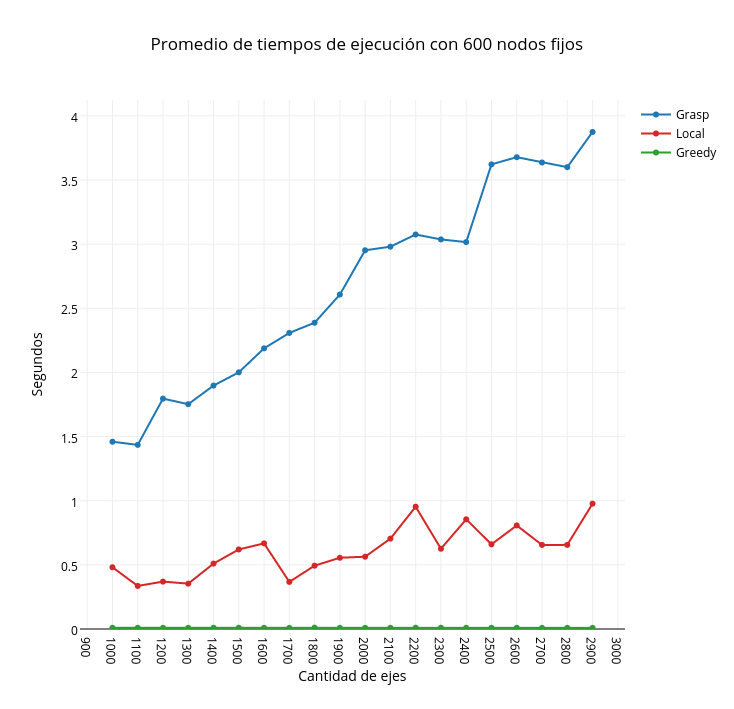
\includegraphics[width=13cm, keepaspectratio=yes]{imagenes/coliseo/Fixnode/600.png}

 	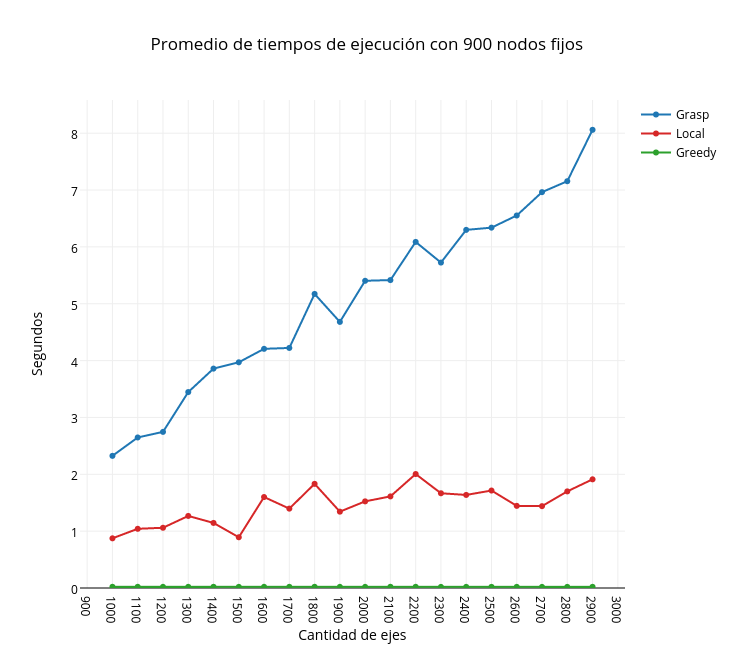
\includegraphics[width=13cm, keepaspectratio=yes]{imagenes/coliseo/Fixnode/900.png}
\end{center}

Se puede observar, que los algoritmos empeoran a mayor cantidad de nodos, pero debe notarse, que en general, Local y Greedy permanecen más bien constantes, mientras que Grasp empeora a mayor cantidad de ejes tiene, en grafos más grandes. 
Por lo tanto, y conforme al análisis anterior, queda aún más claro que para casos grandes, Local es la mejor alternativa al momento de fijar nodos y variar ejes, sea por tiempos de ejecución, como por mejor resultado.

\subsubsection{Ejes Fijos}
Para continuar, realizamos los mismos tests, pero manteniendo los ejes fijos y variando la cantidad de nodos. Los tests realizados fueron con ejes fijos desde 0 hasta 1000 y para cada instancia,
los nodos var\'ian de 50 a 1000.\\

Mostraremos los resultados obtenidos con 300, 600 y 900 ejes fijos:\\

   \begin{center}
 	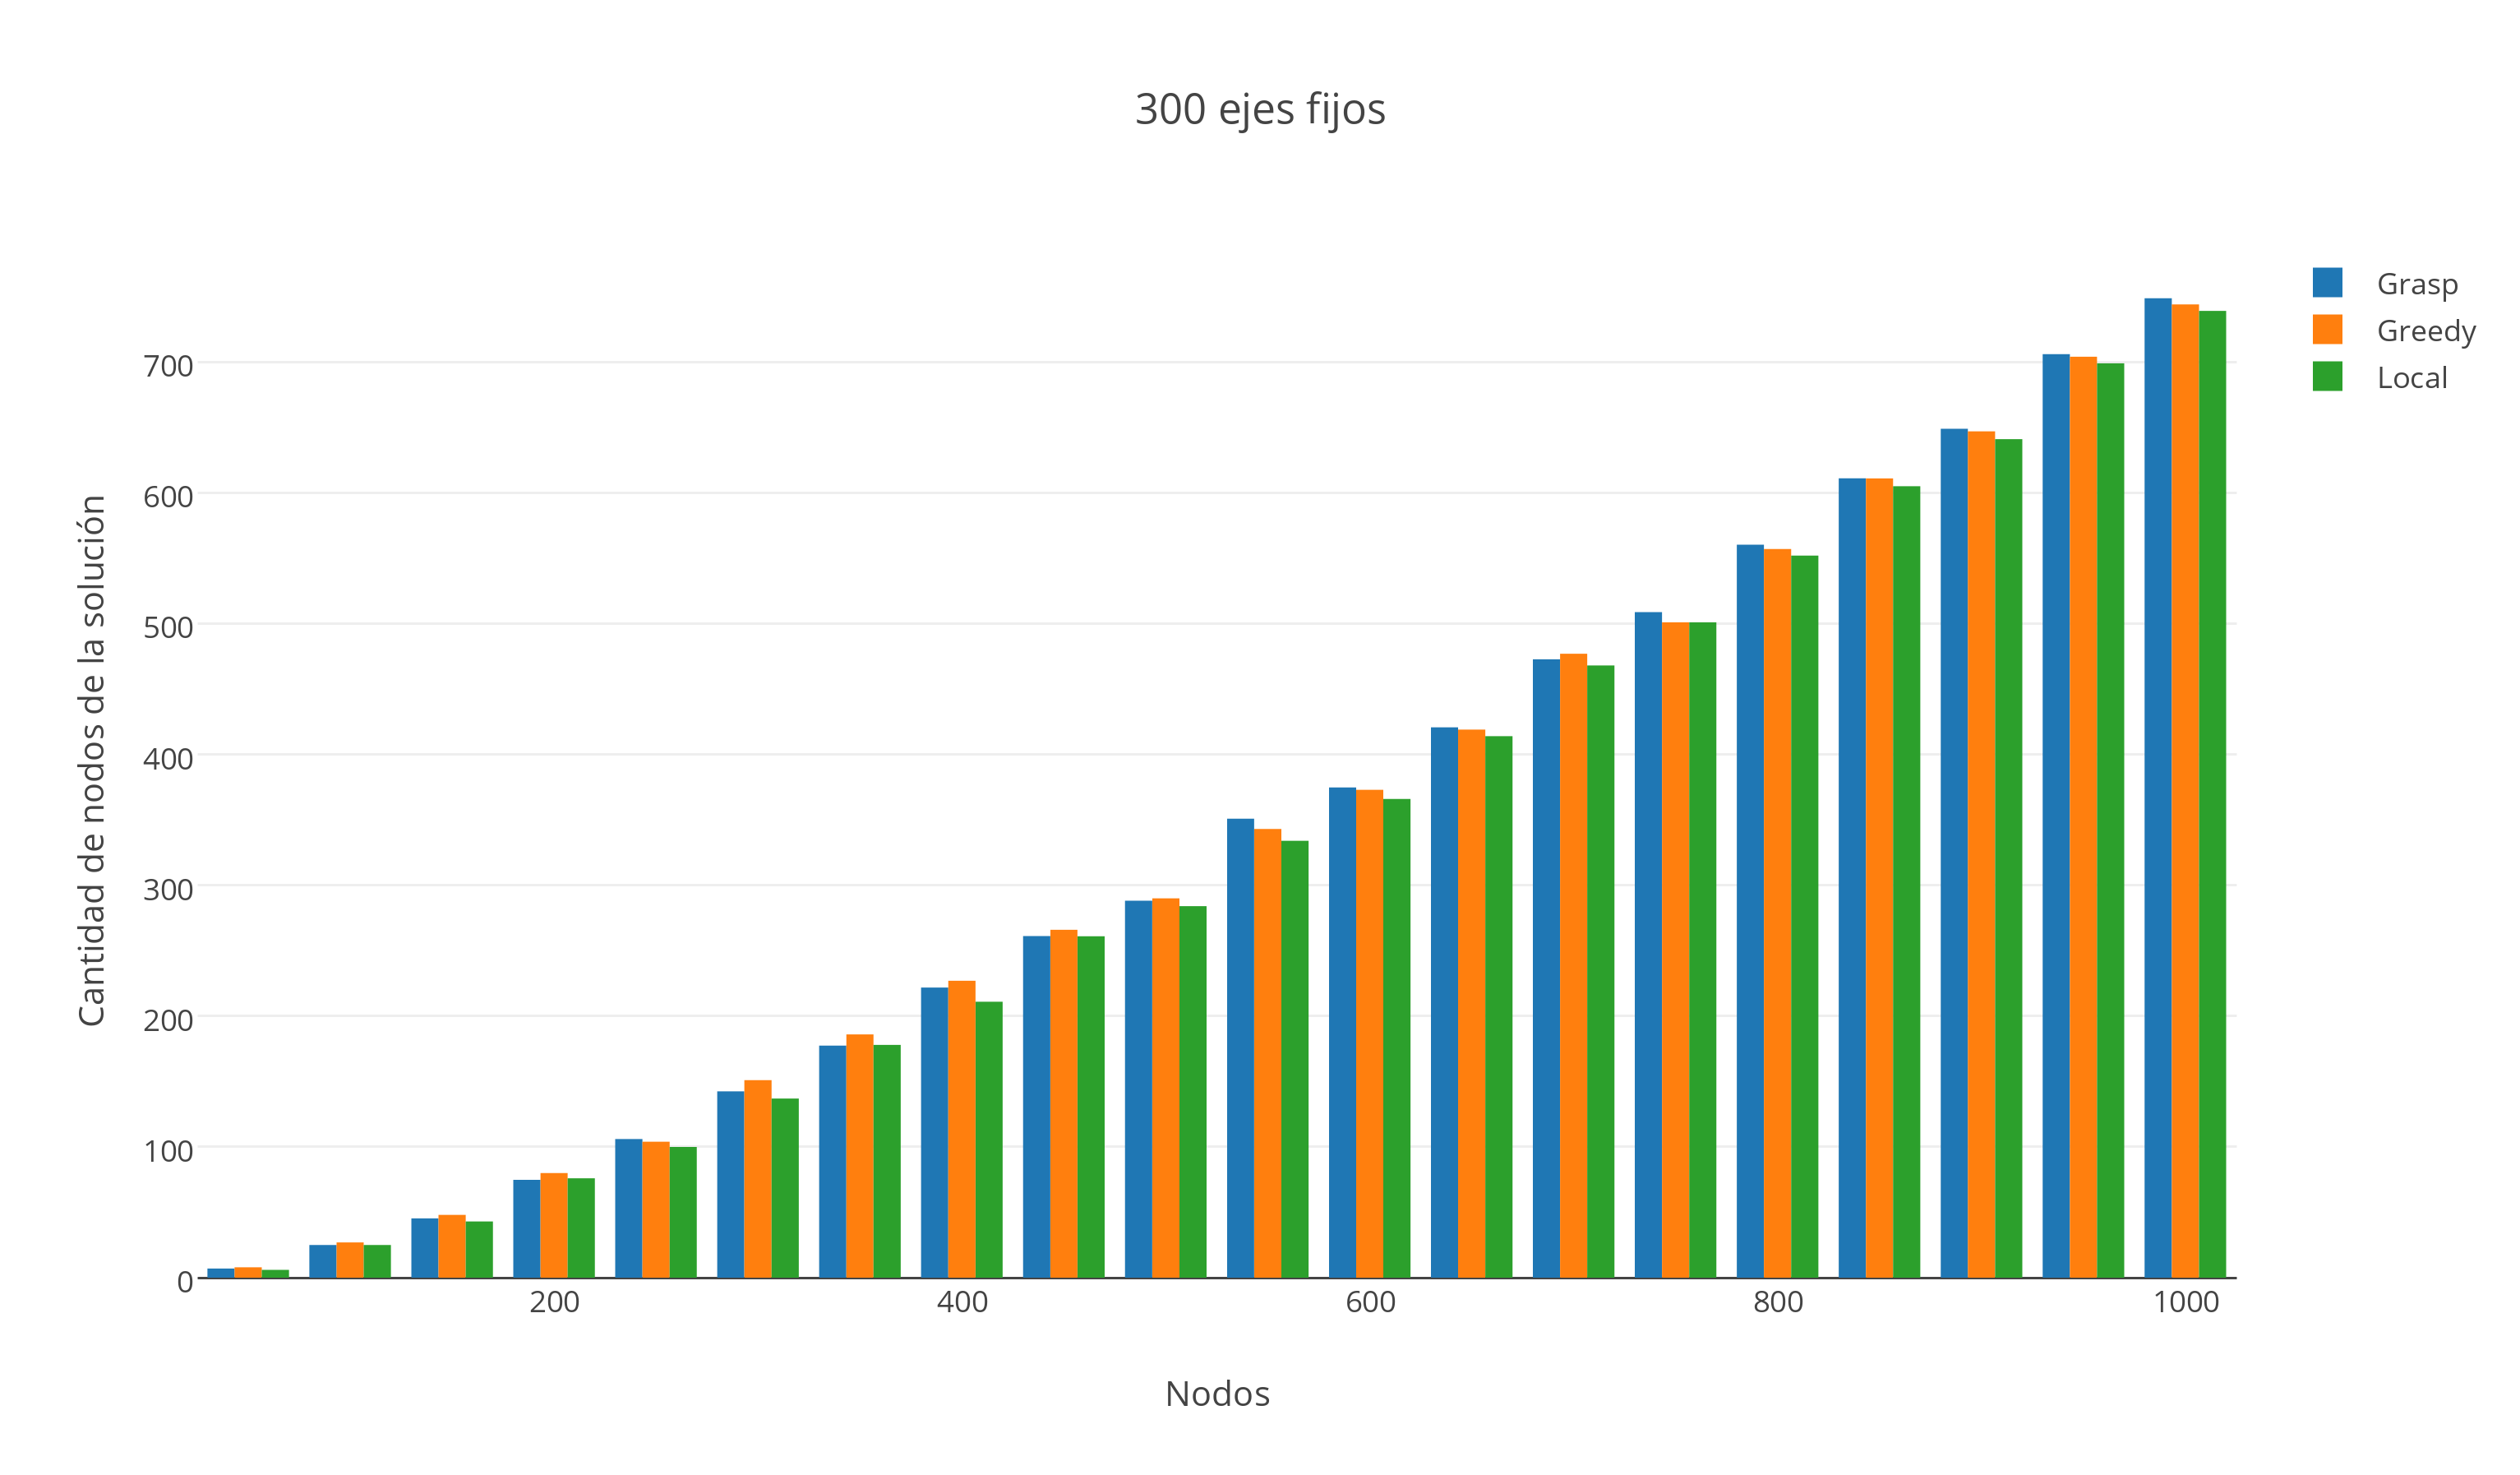
\includegraphics[width=13cm, keepaspectratio=yes]{imagenes/6/300EjesFijos.png}

 	\includegraphics[width=13cm, keepaspectratio=yes]{imagenes/6/600EjesFijos.png}

 	\includegraphics[width=13cm, keepaspectratio=yes]{imagenes/6/900EjesFijos.png}
   \end{center}
 
A primera vista, se puede ver que para casi todas las instancias el algoritmo de B\'usqueda Local es el que menos nodos utiliza en su soluci\'on. 
En cuanto al Greedy y el Grasp, las diferencias son chicas y alternadas con 300 ejes, pero con 600 y 900 ejes, Greedy aparenta ser el peor.\\

Para corroborar estos datos, tomamos nuevamente el promedio de todas las soluciones:\\

\textcolor{red}{Tabla con promedios}
\begin{tabular}{| l | l | l | l |}
   \hline
   Nodos & Grasp & Local & Greedy\\ \hline
   300 & 337.61 & 332 & 338.15 \\ \hline
   600 & 256.165 & 250.4 & 261.8 \\ \hline
   900 & 207.44 & 203.1 & 217.9 \\
   \hline
\end{tabular}

Como preve\'iamos, estos promedios confirman nuestro an\'alisis.

Nuevamente, para fortalecer nuestra conclusión, se analizaron los tiempos de ejecución en las mismas instancias, cuyos resultados fueron los siguientes:

\begin{center}
 	\includegraphics[width=13cm, keepaspectratio=yes]{imagenes/coliseo/Fixedge/0.png}

 	\includegraphics[width=13cm, keepaspectratio=yes]{imagenes/coliseo/Fixedge/300.png}

 	\includegraphics[width=13cm, keepaspectratio=yes]{imagenes/coliseo/Fixedge/600.png}

 	\includegraphics[width=13cm, keepaspectratio=yes]{imagenes/coliseo/Fixedge/900.png}
\end{center}

Como era esperado, Grasp insume mayor tiempo que Local y Greedy para cualquier caso.
Considerando los resultados y los tiempos de ejecución, concluímos que Local es la mejor alternativa, si se mantienen ejes y se varían nodos.

\subsection{Familias específicas}
\subsubsection{Grafo completo}

\textcolor{red}{Diganme si vale la pena hablar sobre grafos completos. Onda, la respuesta es trivial, y los tiempos son meh}

\subsubsection{Grafo bipartito completo}

\textcolor{red}{Brian contandonos un poco los resultados del bipartito completo}
Dado que los resultados siempre son \'optimos, se omitieron los gr\'aficos de resultados para este caso.

Analizando los tiempos de ejecución sobre instancias de 100, 300, 600 y 900 nodos, se obtuvieron los siguientes resultados:

\begin{center}
 	\includegraphics[width=13cm, keepaspectratio=yes]{imagenes/coliseo/Bipartite1.png}

 	\includegraphics[width=13cm, keepaspectratio=yes]{imagenes/coliseo/Bipartite2.png}
\end{center}

\textcolor{red}{Y Ezequiel nos cuenta como esto se debe a los pares de nodos que agarra}.

Para el segundo gráfico, se omitió la ejecución del Grasp, dado que los tiempos de ejecución del mismo para los grafos bipartitos completos de esa magnitud, eran demasiado altos, 
lo cual era predecible pues debe ejecutar la b\'usqueda local 10 veces, es decir que su ejecuci\'on consume \textit{10x(tiempo de b\'usqueda local)}.


Dado que los tres algoritmos siempre obtienen la solución óptima para la familia de grafos bipartitos completos, concluímos que el Greedy es el mejor de los tres para estos casos, ya que es el que menor tiempo insume. 

\subsubsection{Ciclo simple}

\textcolor{red}{Brian contandonos un poco los resultados del ciclo simple}
Por \'ultimo, analizaremos qu\'e ocurre cuando el grafo de entrada es un ciclo. Para ello fuimos generando distintos ciclos, comenzando con 100 nodos y aumentando de a 100 hasta 1000 nodos.\\
Los resultados obtenidos fueron:\\

\begin{center}
 \includegraphics[width=13cm, keepaspectratio=yes]{imagenes/6/Ciclos.png}
\end{center}

Se aprecia r\'apidamente que el Greedy es el peor de los 3 y que los resultados entre el Grasp y Local son muy parejos, siendo Local un poco mejor en los casos m\'as grandes.\\

A su vez, los tiempos de ejecucion sobre las mismas instancias, se obtuvieron los siguientes resultados:

\begin{center}
 	\includegraphics[width=13cm, keepaspectratio=yes]{imagenes/coliseo/Cicle.png}
\end{center}

\textcolor{red}{Coronar esto diciendo quien es mejor (es decir, el que menos tarda entre los que obtienen mejores resultados en promedio)}
Analizando tanto tiempos como resultados obtenidos, concluimos que el algoritmo Local es el m\'as conveniente cuando el grafo es un ciclo, ya que obtiene resultados mucho mejores al Greedy a pesar
de ser un poco m\'as lento. Adem\'as, es mejor que Grasp tanto en tiempo de ejecuci\'on como en el resultado.

\newpage

\section{Anexo}\label{anexo}

\subsection{Ejecuci\'on de los m\'etodos}

Al momento de ejecutar el \texttt{main} se le deben pasar los siguientes par\'ametros acorde a lo deseado:

\begin{itemize}
\item \textbf{0}: \emph{Algortimo Exacto};
\item \textbf{1}: \emph{Heur\'istica Greedy} (con par\'ametros alpha = 0, conAlpha = true);
\item \textbf{2}: \emph{Heur\'istica B\'usqueda local} (soluci\'on inicial por orden de nomenclatura (greedy = false), vecindad 2x1 (vecindad = true));
\item \textbf{3}: \emph{Heur\'istica B\'usqueda local} (soluci\'on inicial greedy (greedy = true), vecindad 2x1 (vecindad = true), alpha = 0);
\item \textbf{4}: \emph{Heur\'istica B\'usqueda local} (soluci\'on inicial por orden de nomenclatura (greedy = false), vecindad 3x1 (vecindad = false));
\item \textbf{5}: \emph{Heur\'istica B\'usqueda local} (soluci\'on inicial greedy (greedy = true), vecindad 3x1 (vecindad = false), alpha = 0);
\item \textbf{6}: \emph{Heur\'istica GRASP} (soluci\'on inicial por pocentaje de mejores (conAlpha = true), vecindad 2x1 (vecindad = true), alpha = input);
\item \textbf{7}:\emph{ Heur\'istica GRASP} (soluci\'on inicial por pocentaje de mejores (conAlpha = true), vecindad 3x1 (vecindad = false), alpha = input);
\item \textbf{8}:\emph{ Heur\'istica GRASP }(soluci\'on inicial por cantidad de mejores (conAlpha = false), vecindad 2x1 (vecindad = true), alpha = input);
\item \textbf{9}: \emph{Heur\'istica GRASP} (soluci\'on inicial por cantidad de mejores (conAlpha = false), vecindad 3x1 (vecindad = false), alpha = input);
\item \textbf{i}: \emph{Imprime} la lista de adyacencia del grafo pasado por input;
\item \textbf{q}: \emph{Finaliza} la ejecuci\'on;
\end{itemize}

\subsection{Generaci\'on de casos de test}\label{instacegen}

\textcolor{red}{Aca hablar un poco de como generamos los grafos para analizar y bla, no hace falta poner codigo ni nada... pero por lo menos contar que hace el generador de instancias. Asi en cada seccion de experimentacion se cita esta seccion}

% \section{Objetivos generales}

% El objetivo de este Trabajo Práctico es ...


% \section{Contexto}

% \begin{figure}
%   \begin{center}
% 	\includegraphics[scale=0.66]{imagenes/logouba.jpg}
% 	\caption{Descripcion de la figura}
% 	\label{nombreparareferenciar}
%   \end{center}
% \end{figure}


% \paragraph{\textbf{Titulo del parrafo} } Bla bla bla bla.
% Esto se muestra en la figura~\ref{nombreparareferenciar}.




%Habra que insertar el enunciado???
% %\section{Enunciado y solucion} 
% %\input{enunciado}

% \section{Conclusiones y trabajo futuro}

\end{document}

